%%%%%%%%%%%%%%%%%%%%%%%%%%%%%%%%%%%%%%%%%%%%%%%%%%%%%%%%%%%%%%%
%% OXFORD THESIS TEMPLATE

% Use this template to produce a standard thesis that meets the Oxford University requirements for DPhil submission
%
% Originally by Keith A. Gillow (gillow@maths.ox.ac.uk), 1997
% Modified by Sam Evans (sam@samuelevansresearch.org), 2007
% Modified by John McManigle (john@oxfordechoes.com), 2015
% Modified by Jason Watson (jason.watson@physics.ox.ac.uk), 2018
%
% This version Copyright (c) 2015-2017 John McManigle
%
% Broad permissions are granted to use, modify, and distribute this software
% as specified in the MIT License included in this distribution's LICENSE file.
%

%%%%% PAGE LAYOUT
% This one will format for two-sided binding (ie left and right pages have mirror margins; blank pages inserted where needed):
%\documentclass[a4paper,twoside]{ociamthesis}
% This one will format for one-sided binding (ie left margin > right margin; no extra blank pages):
\documentclass[a4paper]{ociamthesis}
% This one will format for PDF output (ie equal margins, no extra blank pages):
%\documentclass[a4paper,nobind]{ociamthesis} 


%%%%% PGF
\usepackage{pgf}
%\pgfplotsset{compat=1.12}
\DeclareUnicodeCharacter{2212}{-}


%%%%% DRAFT FOOTER
\fancyfoot[C]{\emph{DRAFT Printed on \today}}  


%%%%% DRAFT CORRECTIONS
% This highlights (in blue) corrections marked with (for words) \mccorrect{blah} or (for whole
% paragraphs) \begin{mccorrection} . . . \end{mccorrection}.  This can be useful for sending a PDF of
% your corrected thesis to your examiners for review.  Turn it off, and the blue disappears.
\correctionstrue


%%%%% BIBLIOGRAPHY SETUP
% Note that your bibliography will require some tweaking depending on your department, preferred format, etc.
% The options included below are just very basic "sciencey" and "humanitiesey" options to get started.
% If you've not used LaTeX before, I recommend reading a little about biblatex/biber and getting started with it.
% If you're already a LaTeX pro and are used to natbib or something, modify as necessary.
% Either way, you'll have to choose and configure an appropriate bibliography format...

% The science-type option: numerical in-text citation with references in order of appearance.
\usepackage[style=numeric-comp, sorting=none, backend=biber]{biblatex}
\newcommand*{\bibtitle}{References}

% This makes the bibliography left-aligned (not 'justified') and slightly smaller font.
\renewcommand*{\bibfont}{\raggedright\small}

% Change this to the name of your .bib file (usually exported from a citation manager like Zotero or EndNote).
\addbibresource{bibtex/articles.bib}
\addbibresource{bibtex/internal.bib}
\addbibresource{bibtex/webpages.bib}


% Uncomment this if you want equation numbers per section (2.3.12), instead of per chapter (2.18):
%\numberwithin{equation}{subsection}


%%%%% THESIS / TITLE PAGE INFORMATION
\title{Calibration and Analysis of the GCT Camera for the Cherenkov Telescope Array}
\author{Jason J. Watson}
\college{Brasenose College}
\degree{Doctor of Philosophy}
\degreedate{Trinity 2018}


%%%%% PERSONAL MACROS
% Commands
\newcommand{\quotes}[1]{``#1''}

% New list method
\newlength{\bulletwidth}\settowidth{\bulletwidth}{$\bullet$}
\newcommand{\mitem}{\setlength{\leftskip}{\leftmargin}\hspace*{-\labelsep}\hspace*{-\bulletwidth}$\bullet$\hspace*{\labelsep}}
\newcommand{\mend}{\setlength{\leftskip}{0cm}}
\newcommand{\utilde}{\raise.17ex\hbox{$\scriptstyle\mathtt{\sim}$}}

% Abbreviations:s
\usepackage[toc,acronym,shortcuts,nopostdot]{glossaries-prefix}
%\newcommand*\glsr[2][]{\glsdisp[#1]{#2}{\glsentryshort{#2} (\glsentrylong{#2})}}
%\newcommand*\glsr[2][]{\glsdisp[#1]{#2}{\glsentryshort{#2} (\glsentrylong{#2})}}
%\newcommand*\glsrpl[2][]{\glsdisp[#1]{#2}{\glsentryshortpl{#2} (\glsentrylongpl{#2})}}
%from documentation
%\newacronym[⟨key-val list⟩]{⟨label ⟩}{⟨abbrv ⟩}{⟨long⟩}
%above is short version of this
% \newglossaryentry{⟨label ⟩}{type=\acronymtype,
% name={⟨abbrv ⟩},
% description={⟨long⟩},
% text={⟨abbrv ⟩},
% first={⟨long⟩ (⟨abbrv ⟩)},
% plural={⟨abbrv ⟩\glspluralsuffix},
% firstplural={⟨long⟩\glspluralsuffix\space (⟨abbrv ⟩\glspluralsuffix)},
% ⟨key-val list⟩}

%\newacronym{api}{API}{Application Programming Interface }

\newacronym{fwhm}{FWHM}{Full Width at Half Maximum}
\newacronym{vhe}{VHE}{Very High Energy}
\newacronym{psf}{PSF}{Point Spread Function}
\newacronym[prefix={an~}]{nsb}{NSB}{Night-Sky Background}
\newacronym{dcr}{DCR}{Dark-Count Rate}
\newacronym{pe}{p.e.}{Photo-Electrons}
\newacronym{adc}{ADC}{Analogue-to-Digital Converter}
\newacronym{pde}{PDE}{Photon Detection Efficiency}
\newacronym{qe}{QE}{Quantum Efficiency}
\newacronym{spe}{SPE}{Single Photo-Electron}
\newacronym{eso}{ESO}{European Southern Observatory}
\newacronym{iact}{IACT}{Imaging Atmospheric Cherenkov Telescope}
\newacronym[prefixfirst={the~}]{cta}{CTA}{Cherenkov Telescope Array}
\newacronym{lst}{LST}{Large Size Telescope}
\newacronym{mst}{MST}{Medium Size Telescope}
\newacronym{sst}{SST}{Small Size Telescope}
\newacronym{sct}{SCT}{Schwarzschild-Couder Telescope}
\newacronym[prefixfirst={the~}]{gct}{GCT}{Gamma-ray Cherenkov Telescope}
\newacronym[prefixfirst={the~}]{chec}{CHEC}{Compact High Energy Camera}
\newacronym[prefixfirst={the~}]{chec-m}{CHEC-M}{\gls{chec} using \glspl{mapmt} as the detector}
\newacronym[prefixfirst={the~}]{chec-s}{CHEC-S}{\gls{chec} using \glspl{sipmt} as the detector}
\newacronym{pmt}{PMT}{Photomultiplier Tube}
\newacronym{mapmt}{MAPMT}{Multi-Anode Photomultiplier Tube}
\newacronym{sipmt}{SiPMT}{Silicon Photomultiplier Tube}
\newacronym{target5}{TARGET~5}{\gls{target} (version 5)}
\newacronym{targetc}{TARGET~C}{\gls{target} (version C)}
\newacronym{fpga}{FPGA}{Field-Programmable Gate Array}
\newacronym{adc2pe}{adc2pe}{conversion of \gls{adc} counts to \gls{pe}}
\newacronym{mc}{MC}{Monte-Carlo}
\newacronym{hv}{HV}{High Voltage}
\newacronym{impact}{ImPACT}{Image Pixel-wise fit for Atmospheric Cherenkov Telescopes}
\newacronym{fee}{FEE}{Front-End Electronics}
\newacronym{dc}{DC}{Direct Current}
\newacronym{ac}{AC}{Alternating Current}
\newacronym{rmse}{RMSE}{Root-Mean-Square Error}
\newacronym{oes}{OES}{Observation Execution System}
\newacronym{dpps}{DPPS}{Data Processing and Preservation System}
\newacronym{suss}{SUSS}{Science User Support System}
\newacronym{irf}{IRF}{Instrument Response Function}

\newglossaryentry{target}{type=\acronymtype, 
	name={TARGET}, 
	description={TeV Array Readout with GSa/s sampling and Event Trigger}, 
	first={TARGET (TeV Array Readout with GSa/s sampling and Event Trigger)}
}
\newglossaryentry{asic}{type=\acronymtype, 
	name={ASIC}, 
	description={Application-Specific Integrated Circuit}, 
	first={ASIC (Application-Specific Integrated Circuit)}
}
\newglossaryentry{vped}{type=\acronymtype, 
	name={Vped}, 
	description={Pedestal voltage input into the TARGET ASIC}, 
	first={input pedestal voltage (Vped)}
}
\newglossaryentry{fits}{type=\acronymtype, 
	name={FITS}, 
	description={Flexible Image Transport System}, 
	first={FITS (Flexible Image Transport System)}
}
\newglossaryentry{swig}{type=\acronymtype, 
	name={SWIG}, 
	description={Simplified Wrapper and Interface Generator}, 
	first={SWIG (Simplified Wrapper and Interface Generator)}
}
\newglossaryentry{tio}{type=\acronymtype, 
	name={TIO}, 
	description={Custom fits file format defined by TargetIO used for storing waveform data from TARGET-based cameras}, 
	first={TIO}
}
\newglossaryentry{astri}{type=\acronymtype, 
	name={ASTRI}, 
	description={Astrofisica con Specchi a Tecnologia Replicante Italiana}, 
	first={ASTRI (Astrofisica con Specchi a Tecnologia Replicante Italiana)}
}
\newglossaryentry{citiroc}{type=\acronymtype, 
	name={CITIROC}, 
	description={Cherenkov Imaging Telescope Integrated Read Out Chip}, 
	first={CITIROC (Cherenkov Imaging Telescope Integrated Read Out Chip)}
}
\newglossaryentry{aerie}{type=\acronymtype, 
	name={AERIE}, 
	description={Analysis and Event Reconstruction Integrated Environment}, 
	first={AERIE (Analysis and Event Reconstruction Integrated Environment)}
}
\newglossaryentry{corsika}{type=\acronymtype, 
	name={CORSIKA}, 
	description={COsmic Ray SImulations for KAscade}, 
	first={CORSIKA (COsmic Ray SImulations for KAscade)}
}
\newglossaryentry{kascade}{type=\acronymtype, 
	name={KASCADE}, 
	description={KArlsruhe Shower Core and Array DEtector}, 
	first={KASCADE (KArlsruhe Shower Core and Array DEtector)}
}
\newglossaryentry{hess}{type=\acronymtype, 
	name={H.E.S.S.}, 
	description={High Energy Stereoscopic System}, 
	first={H.E.S.S. (High Energy Stereoscopic System)}
}
\newglossaryentry{magic}{type=\acronymtype, 
	name={MAGIC}, 
	description={Major Atmospheric Gamma Imaging Cherenkov Telescopes}, 
	first={MAGIC (Major Atmospheric Gamma Imaging Cherenkov Telescopes)}
}
\newglossaryentry{veritas}{type=\acronymtype, 
	name={VERITAS}, 
	description={Very Energetic Radiation Imaging Telescope Array System}, 
	first={VERITAS (Very Energetic Radiation Imaging Telescope Array System)}
}
\newglossaryentry{hawc}{type=\acronymtype, 
	name={HAWC}, 
	description={High-Altitude Water Cherenkov observatory}, 
	first={HAWC (High-Altitude Water Cherenkov observatory)}
}
\newglossaryentry{udp}{type=\acronymtype, 
	name={UDP}, 
	description={User Datagram Protocol}, 
	first={UDP (User Datagram Protocol)}
}

% \newcommand{\glsf}[1]{\glsunset{#1}\glsentryfull{#1}}
% \newcommand{\glsfpl}[1]{\glsunset{#1}\glsentryfullpl{#1}}
\newcommand*{\glsb}[2][]{\ifglsused{#2}{\acs[#1]{#2}}{%
 \glsunset{#2}%
 \acl[#1]{#2} [\acs[#1]{#2}]}}

% Nomenclature:
%\newglossaryentry{angelsperarea}{
%	name = $a$ ,
%	description = The number of angels per unit area,
%}
\makeglossaries

% To make text superscripts shortcuts
\renewcommand{\th}{\textsuperscript{th}} % ex: I won 4\th place
\newcommand{\nd}{\textsuperscript{nd}}
\renewcommand{\st}{\textsuperscript{st}}
\newcommand{\rd}{\textsuperscript{rd}}

\usepackage{xargs}
\usepackage[colorinlistoftodos,prependcaption,textsize=tiny]{todonotes}
\newcommandx{\change}[2][1=]{\todo[linecolor=red,backgroundcolor=red!25,bordercolor=red,#1]{#2}}
\newcommandx{\otherch}[2][1=]{\todo[linecolor=purple,backgroundcolor=purple!25,bordercolor=purple,#1]{#2}}
\newcommandx{\final}[2][1=]{\todo[linecolor=green,backgroundcolor=green!25,bordercolor=green,#1]{#2}}
\newcommandx{\notes}[2][1=]{\todo[linecolor=gray,backgroundcolor=gray!25,bordercolor=gray,#1]{#2}}
\newcommandx{\thiswillnotshow}[2][1=]{\todo[disable,#1]{#2}}

\usepackage{booktabs}

\usepackage{rotating}

\usepackage{listings}
\lstset{
	frameround=fttt,
	language=C++,
	breaklines=true,
	keywordstyle=\color{gray}\bfseries, 
	basicstyle=\ttfamily\color{gray},
	numberstyle=\color{black}
}
\lstset{ %
language=C++,                % choose the language of the code
basicstyle=\footnotesize,       % the size of the fonts that are used for the code
numbers=left,                   % where to put the line-numbers
numberstyle=\footnotesize,      % the size of the fonts that are used for the line-numbers
stepnumber=1,                   % the step between two line-numbers. If it is 1 each line will be numbered
numbersep=8pt,                  % how far the line-numbers are from the code
backgroundcolor=\color{white},  % choose the background color. You must add \usepackage{color}
showspaces=false,               % show spaces adding particular underscores
showstringspaces=false,         % underline spaces within strings
showtabs=false,                 % show tabs within strings adding particular underscores
frame=single,           % adds a frame around the code
tabsize=2,          % sets default tabsize to 2 spaces
captionpos=b,           % sets the caption-position to bottom
breaklines=true,        % sets automatic line breaking
breakatwhitespace=false,    % sets if automatic breaks should only happen at whitespace
escapeinside={\%*}{*)},          % if you want to add a comment within your code
xleftmargin=1.5em,
framexleftmargin=0.1em
}
\newcommand{\pkg}[1]{\texttt{#1}}
\newcommand{\cpp}{{C\nolinebreak[4]\hspace{-.05em}\raisebox{.4ex}{\tiny\bf ++}}}
\lstMakeShortInline[columns=fixed]|

\newcommand*\average[1]{\bar{#1}}
%\newcommand{\unit}[1]{\ensuremath{\, \mathrm{#1}}}
\newcommand{\me}{\mathrm{e}}

\usepackage{textgreek}
\usepackage{siunitx}
\DeclareSIUnit{\pe}{{p.e.}}
\sisetup{range-phrase=-, range-units=single}

\usepackage{float}
\usepackage[most]{tcolorbox}
%\tcbset{enhanced,colback=white,colframe=gray!75!black,fonttitle=\bfseries}
\newtcolorbox{requirement}[2][]{
    %float=htb,
    colback=white, 
    colframe=gray!75!black,
    every float=\centering,
    lower separated=false,
    fonttitle=\bfseries, 
    title={#2},
    #1
}
\newcommand{\requirementref}[1]{\textbf{#1}}

\usepackage{graphicx,wrapfig,lipsum}
\usepackage{subcaption}

\newcommand{\hangpara}{
 \setlength{\parindent}{0cm} % don't indent new paragraphs
 \hangindent=0.8cm % indent all subsequent lines
}

\graphicspath{
	{figures/}
	{figures/ch1/}
	{figures/ch2/}
	{figures/ch3/}
	{figures/ch4/}
	{figures/ch5/}
	{figures/ch6/}
	{figures/ch7/}
	{figures/ch8/}
	{figures/ch9/}
	{figures/a1/}
	{figures/a2/}
    {figures/a3/}
    {figures/a4/}
    {figures/a5/}
}

%\usepackage{lineno}
%\linenumbers
%\raggedbottom % Don't stretch line spacing to fill page

\begin{document}


%%%%% LINE SPACING
% OFFICIAL
\setlength{\textbaselineskip}{22pt plus2pt}
% DRAFT
%\setlength{\textbaselineskip}{18pt plus2pt minus1pt}


%%%%% LINE SPACING (roman-numbered pages)
\setlength{\frontmatterbaselineskip}{17pt plus1pt minus1pt}

% Leave this line alone; it gets things started for the real document.
\setlength{\baselineskip}{\textbaselineskip}


%%%%% SECTION NUMBERING DEPTH
% You have two choices.  First, how far down are sections numbered?  (Below that, they're named but
% don't get numbers.)  Second, what level of section appears in the table of contents?  These don't have
% to match: you can have numbered sections that don't show up in the ToC, or unnumbered sections that
% do.  Throughout, 0 = chapter; 1 = section; 2 = subsection; 3 = subsubsection, 4 = paragraph...
% The level that gets a number:
\setcounter{secnumdepth}{2}
% The level that shows up in the ToC:
\setcounter{tocdepth}{2}


%%%%% ABSTRACT SEPARATE
\begin{abstractseparate}
	The interaction of very high energy gamma rays with the Earth's atmosphere produces extensive electromagnetic particle cascades. This superluminal shower of particles emits photons of blue wavelength, commonly known as Cherenkov radiation. The \gls{iact} technique enables the probing of the universe at \si{TeV} energies through the detection of these Cherenkov showers. The \gls{cta} will represent the next leap forward in \gls{vhe} astronomy, improving on the sensitivity of current \glspl{iact} by a factor of 10, encompassing energies from \SI{20}{GeV} to \SI{300}{TeV}, and operating as the first open observatory in this field. A major component of \gls{cta} are the \glspl{sst}, a necessary ingredient in exploring past the present energy frontier in gamma-ray astronomy.

One of three proposed designs for the \gls{sst} is the \gls{gct}. Utilising a dual-mirror Schwarzschild-Couder optical design, \gls{gct} enables a \SI{9}{\degree} \gls{fov} for a compact camera design. The camera developed for \gls{gct} is the \gls{chec}. Two prototypes for \gls{chec} have been built, each utilising different compact photosensor technology. \gls{chec-m} features \glspl{mapmt}, a pixelised extension of the \gls{pmt} technology extensively used by \glspl{iact}. \mbox{\gls{chec-s}} features \glspl{sipmt}, a novel photosensor which utilises semiconductor technology for high resolution photon counting over a large dynamic range. To fully utilise the signal output from these photosensors, and allow the opportunity for future data analysis procedures to be exploited, the entire signal received from these photosensors are digitised into waveforms following a trigger. These waveforms have a length of 96 samples with nanosecond precision.

In this thesis, the full calibration and signal-extraction pipeline currently adopted by \gls{chec} to reliably extract the Cherenkov signal from the waveforms is presented. The resulting performance of these procedures, and of the camera designs, is explored with respect to the requirements specified by the \gls{cta} Observatory. Potential improvements to the camera and calibration implementations are identified, and simulations of \gls{chec} are utilised to demonstrate the performance increase these proposals provide. Consequently, an improvement to the photosensor that would allow the \gls{chec-s} prototype design to comfortably meet the \gls{cta} requirements is specified. Testing of these improvements is anticipated to commence in early 2019. Finally, the results of the second on-telescope campaign for the \gls{chec-m} prototype are presented, during which observations of Cherenkov showers and optical measurements of Jupiter were conducted.
\end{abstractseparate}
\glsresetall


\begin{romanpages}


%%%%% TITLEPAGE
\maketitle

%%%%% DEDICATION -- If you'd like one, un-comment the following.
%\begin{dedication}
%This thesis is dedicated to\\
%someone\\
%for some special reason\\
%\end{dedication}

%%%%% ACKNOWLEDGEMENTS
\begin{acknowledgements}
 	\subsection*{Personal}

Lorem ipsum dolor sit amet, consectetur adipiscing elit. Vestibulum feugiat et est at accumsan. Praesent sed elit mattis, congue mi sed, porta ipsum. In non ullamcorper lacus. Quisque volutpat tempus ligula ac ultricies. Nam sed erat feugiat, elementum dolor sed, elementum neque. Aliquam eu iaculis est, a sollicitudin augue. Cras id lorem vel purus posuere tempor. Proin tincidunt, sapien non dictum aliquam, ex odio ornare mauris, ultrices viverra nisi magna in lacus. Fusce aliquet molestie massa, ut fringilla purus rutrum consectetur. Nam non nunc tincidunt, rutrum dui sit amet, ornare nunc. Donec cursus tortor vel odio molestie dignissim. Vivamus id mi erat. Duis porttitor diam tempor rutrum porttitor. Lorem ipsum dolor sit amet, consectetur adipiscing elit. Sed condimentum venenatis consectetur. Lorem ipsum dolor sit amet, consectetur adipiscing elit.

Aenean sit amet lectus nec tellus viverra ultrices vitae commodo nunc. Mauris at maximus arcu. Aliquam varius congue orci et ultrices. In non ipsum vel est scelerisque efficitur in at augue. Nullam rhoncus orci velit. Duis ultricies accumsan feugiat. Etiam consectetur ornare velit et eleifend.

Suspendisse sed enim lacinia, pharetra neque ac, ultricies urna. Phasellus sit amet cursus purus. Quisque non odio libero. Etiam iaculis odio a ex volutpat, eget pulvinar augue mollis. Mauris nibh lorem, mollis quis semper quis, consequat nec metus. Etiam dolor mi, cursus a ipsum aliquam, eleifend venenatis ipsum. Maecenas tempus, nibh eget scelerisque feugiat, leo nibh lobortis diam, id laoreet purus dolor eu mauris. Pellentesque habitant morbi tristique senectus et netus et malesuada fames ac turpis egestas. Nulla eget tortor eu arcu sagittis euismod fermentum id neque. In sit amet justo ligula. Donec rutrum ex a aliquet egestas.

\subsection*{Institutional}

Lorem ipsum dolor sit amet, consectetur adipiscing elit. Ut luctus tempor ex at pretium. Sed varius, mauris at dapibus lobortis, elit purus tempor neque, facilisis sollicitudin felis nunc a urna. Morbi mattis ante non augue blandit pulvinar. Quisque nec euismod mauris. Nulla et tellus eu nibh auctor malesuada quis imperdiet quam. Sed eget tincidunt velit. Cras molestie sem ipsum, at faucibus quam mattis vel. Quisque vel placerat orci, id tempor urna. Vivamus mollis, neque in aliquam consequat, dui sem volutpat lorem, sit amet tempor ipsum felis eget ante. Integer lacinia nulla vitae felis vulputate, at tincidunt ligula maximus. Aenean venenatis dolor ante, euismod ultrices nibh mollis ac. Ut malesuada aliquam urna, ac interdum magna malesuada posuere.



\subsection*{CTA}
ctapipe, target, chec.....
\end{acknowledgements}

%%%%% ABSTRACT
\begin{abstract}
	The interaction of very high energy gamma rays with the Earth's atmosphere produces extensive electromagnetic particle cascades. This superluminal shower of particles emits photons of blue wavelength, commonly known as Cherenkov radiation. The \gls{iact} technique enables the probing of the universe at \si{TeV} energies through the detection of these Cherenkov showers. The \gls{cta} will represent the next leap forward in \gls{vhe} astronomy, improving on the sensitivity of current \glspl{iact} by a factor of 10, encompassing energies from \SI{20}{GeV} to \SI{300}{TeV}, and operating as the first open observatory in this field. A major component of \gls{cta} are the \glspl{sst}, a necessary ingredient in exploring past the present energy frontier in gamma-ray astronomy.

One of three proposed designs for the \gls{sst} is the \gls{gct}. Utilising a dual-mirror Schwarzschild-Couder optical design, \gls{gct} enables a \SI{9}{\degree} \gls{fov} for a compact camera design. The camera developed for \gls{gct} is the \gls{chec}. Two prototypes for \gls{chec} have been built, each utilising different compact photosensor technology. \gls{chec-m} features \glspl{mapmt}, a pixelised extension of the \gls{pmt} technology extensively used by \glspl{iact}. \mbox{\gls{chec-s}} features \glspl{sipmt}, a novel photosensor which utilises semiconductor technology for high resolution photon counting over a large dynamic range. To fully utilise the signal output from these photosensors, and allow the opportunity for future data analysis procedures to be exploited, the entire signal received from these photosensors are digitised into waveforms following a trigger. These waveforms have a length of 96 samples with nanosecond precision.

In this thesis, the full calibration and signal-extraction pipeline currently adopted by \gls{chec} to reliably extract the Cherenkov signal from the waveforms is presented. The resulting performance of these procedures, and of the camera designs, is explored with respect to the requirements specified by the \gls{cta} Observatory. Potential improvements to the camera and calibration implementations are identified, and simulations of \gls{chec} are utilised to demonstrate the performance increase these proposals provide. Consequently, an improvement to the photosensor that would allow the \gls{chec-s} prototype design to comfortably meet the \gls{cta} requirements is specified. Testing of these improvements is anticipated to commence in early 2019. Finally, the results of the second on-telescope campaign for the \gls{chec-m} prototype are presented, during which observations of Cherenkov showers and optical measurements of Jupiter were conducted.
\end{abstract}
\glsresetall

%%%%% MINI TABLES OF CONTENTS
\dominitoc


% This aligns the bottom of the text of each page.  It generally makes things look better.
\flushbottom


%%%%% TABLE OF CONTENTS
\tableofcontents


%%%%% LIST OF FIGURES
\listoffigures \mtcaddchapter


%%%%% LIST OF ABBREVIATIONS
\newpage
\printglossary[nonumberlist,type=\acronymtype,title=Abbreviations] \mtcaddchapter
\newpage
\printglossary[nonumberlist,type=main,title=Glossary] \mtcaddchapter


\end{romanpages}


%%%%% CHAPTERS
\flushbottom
%\adjustmtc
%\adjustmtc
   \chapter{\label{ch1-intro}Introduction} 

\minitoc

\section{Cherenkov Radiation}

\begin{figure}
  \begin{subfigure}[b]{0.49\textwidth}
    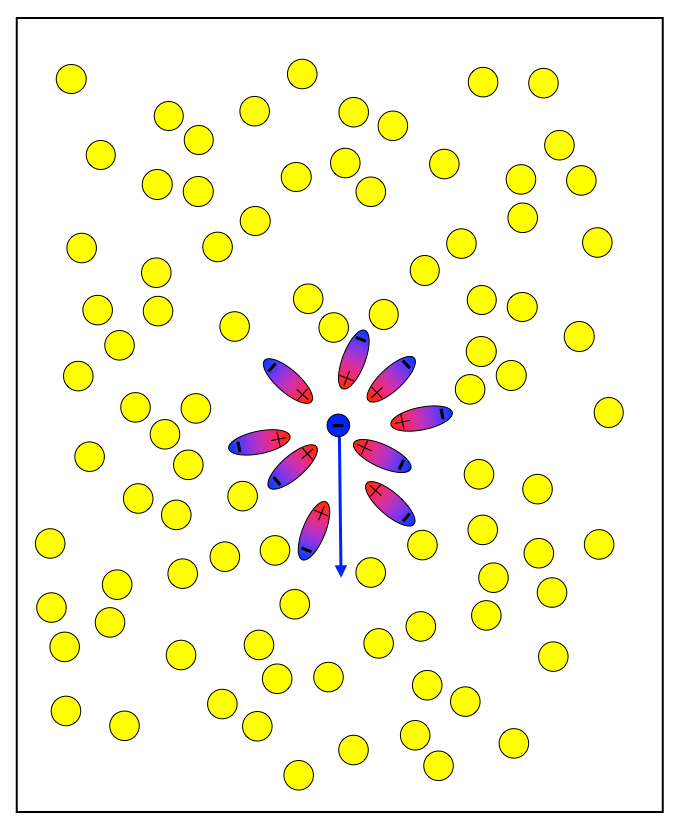
\includegraphics[width=\textwidth]{dipole_slow}
    \caption{$v < \frac{c}{n}$}
    \label{fig:dipole_slow}
  \end{subfigure}
  \hfill
  \begin{subfigure}[b]{0.49\textwidth}
    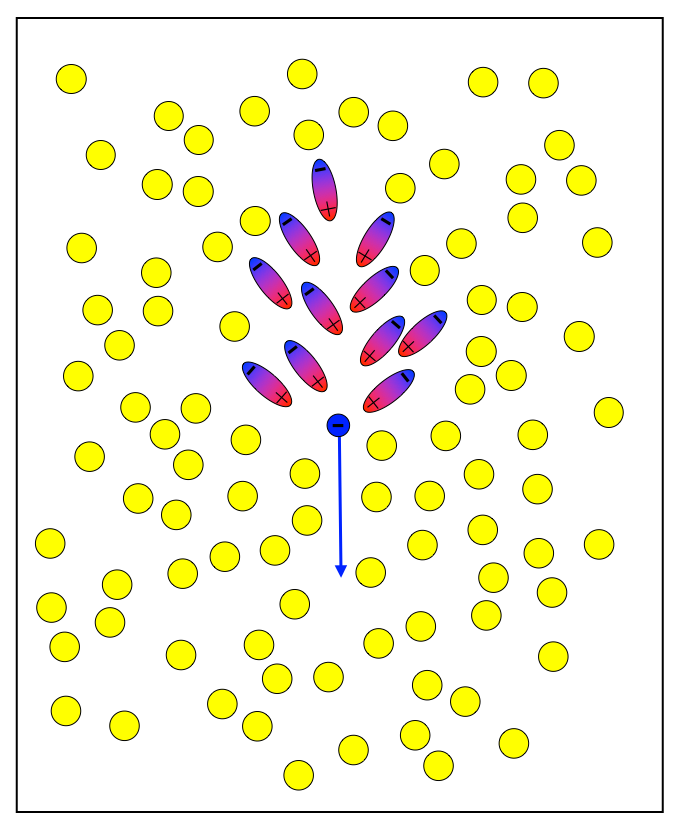
\includegraphics[width=\textwidth]{dipole_fast}
    \caption{$v \ge \frac{c}{n}$}
    \label{fig:dipole_fast}
  \end{subfigure}
  \caption[Polarisation produced in a dielectric medium due to the presence of a charged particle.]{Polarisation produced in a dielectric medium due to the presence of a charged particle, for the cases of a non-relativistic and relativistic particle.}
\end{figure}

\begin{figure}
	\centering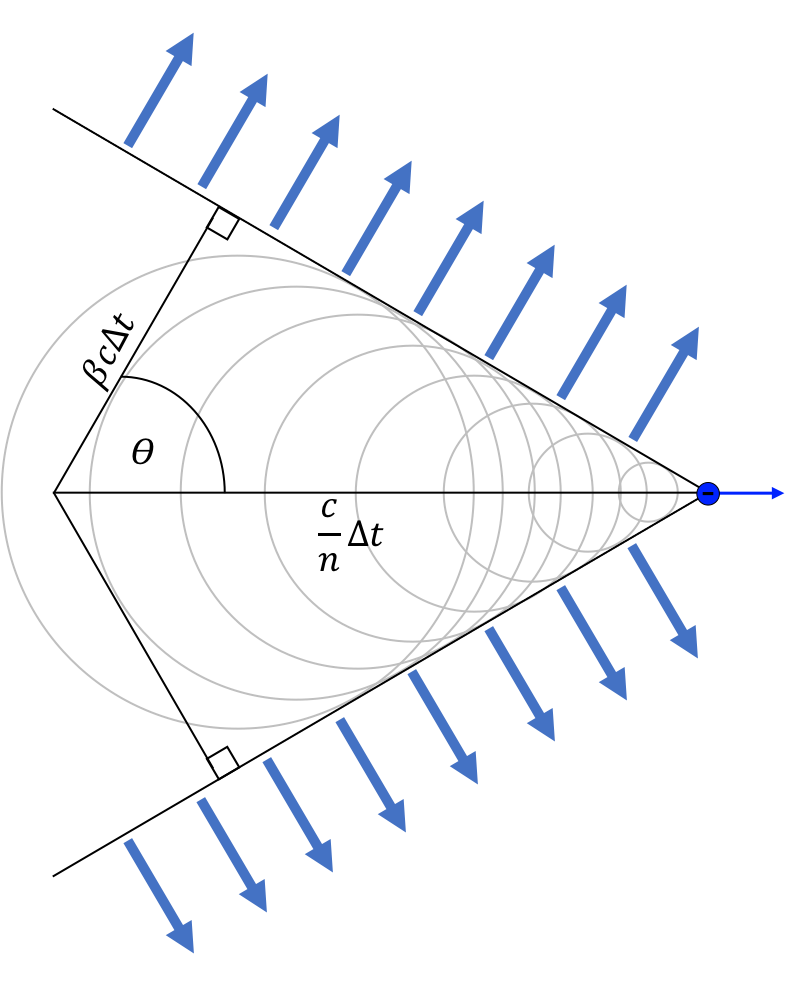
\includegraphics[width=0.5\textwidth]{cherenkov_geom} 
	\caption[Geometry of the wavefronts involved in Cherenkov radiation production.]{Geometry of the wavefronts involved in Cherenkov radiation production. The particle travels at a greater speed than the wavefronts propagate.}
	\label{fig:cherenkov_geom}
\end{figure}

When a charged particle moves slowly through a dielectric medium, the electric field of the particle distorts the nearby atoms. Momentarily, these atoms are transformed into elementary dipoles where the charged particles that constitute the atom are arranged with respect to the electric field of the travelling particle (Figure~\ref{fig:dipole_slow}). Due to the complete symmetry of this polarisation around the travelling particle, no net field is produced by the dielectric medium. However, if instead the velocity of the charged particle is faster than the speed light travels in that medium, an asymmetry along the particle trajectory is formed in the polarisation of the surrounding atoms (Figure~\ref{fig:dipole_fast}), resulting in a net dipole field. As the particle continues through the medium, elements of the polarised medium will release a brief burst of electromagnetic radiation. Generally these electromagnetic waves interfere destructively, except inside in the forward direction along the particles trajectory in an opening angle $\theta$. Although the full characterisation of this relativistic effect is complex, a simple consideration of the geometry involved, shown in Figure~\ref{fig:cherenkov_geom}, can be used to describe $\theta$ \cite{Jelley1958a}. In a time $\Delta t$ a particle travels a distance $\beta c \Delta t$ where $\beta = \frac{v}{c}$, while the emitted light will travel a distance $\frac{c}{n} \Delta t$ in a medium with refractive index $n$. This results in the relation:
\begin{equation} \label{eq:cherenkov_angle}
\cos \theta = \frac{vn}{c}.
\end{equation}
The blue light emitted in this constrained opening angle, via this phenomena, is known as Cherenkov radiation.

\section{Atmospheric Cherenkov Showers} \label{section:cherenkov_shower_intro}

\begin{figure}
	\centering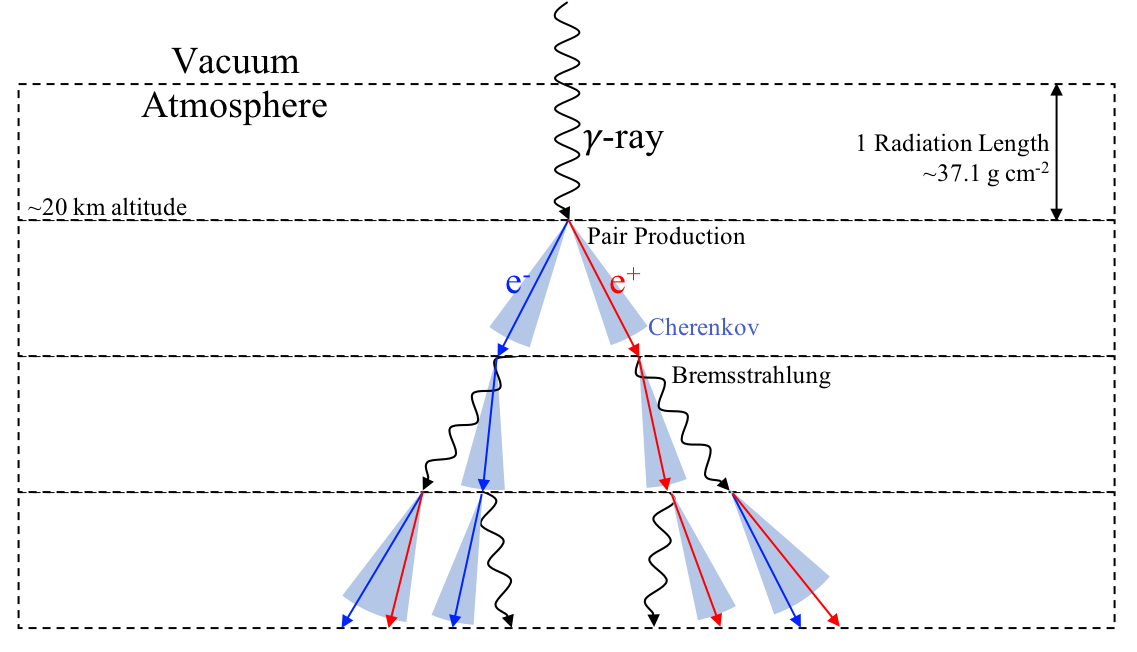
\includegraphics[width=\textwidth]{cascade} 
	\caption[Production of a extended electromagnetic particle cascade.]{Production of a extended electromagnetic particle cascade, demonstrating the different components and interactions.}
	\label{fig:cascade}
\end{figure}

The Earth's atmosphere is effectively opaque to photon energies above \SI{10}{eV} \cite{Weekes2003}. To conduct astronomical observations at higher energies, one must usually leave the Earth's atmosphere. However, at energies above \SI{\ge 10}{GeV}, a ``gamma-ray window'' exists where the pursuit of gamma-ray observations can be performed using the Cherenkov radiation produced by the cascade of particles resulting from the interaction between the gamma ray and the atmosphere.

Two electromagnetic interactions are responsible for the creation of this cascade:
\begin{description}
\item [Pair Production] The conversion of a photon into an electron-positron pair in the presence of an atom (such as an atmospheric particle). The energy of the photon must exceed the sum of the rest masses of an electron and positron (\SI{1.022}{MeV}). The electron-positron pair share the energy of the progenitor photon, and continue on a similar trajectory. This is the dominating interaction process for photons above \SI{\ge 10}{MeV} \cite{Weekes2003}.
\item [Bremsstrahlung radiation] The emission of a photon due to the interaction of a charged particle with the electric field on an atom (such as an atmospheric particle). This process allows further gamma rays to be produced.
\end{description}
The interplay between these two processes, occurring after each transversal of a radiation length, produces the extensive cascade of energetic electromagnetic particles. This is illustrated in Figure~\ref{fig:cascade}. The charged particles produced by the pair production in this cascade are responsible for the generation of the Cherenkov light. This cascade is often known as a ``Cherenkov shower''.

This cascade continues until the ionisation energy losses are equal to the radiation losses. The number of remaining particles after this point, known as the ``shower maximum'', begins to diminish. For a \SI{1}{TeV} shower this occurs at \SI{\sim 8.4}{km} altitude~\cite{Weekes2003}. The produced Cherenkov light is collimated along the progenitor gamma ray trajectory, and produces a pool of blue light on the ground, with a radius of \SI{\sim 120}{m}~\cite{Hillas1996a}. If the direction of the Cherenkov shower is extrapolated back to the cosmic sphere, the location of the source that produced the gamma ray can be inferred. Although the amount of energy that goes into Cherenkov photon production is a tiny fraction of the total energy, the atmosphere acts as a consistent calorimeter, therefore allowing an accurate reconstruction of the progenitors energy from the amount of Cherenkov photons produced. 

A further characteristic of the Cherenkov shower is the time profile. The entire shower typically lasts \SI{\sim 5}{ns}. Therefore, despite the abundance of showers in the sky, and the visible wavelength of the Cherenkov light, they are imperceivable by the human eye. Furthermore, due to the faster-than-light velocities of the particles inside the cascade, the last Cherenkov photons produced at the end of the shower reach the ground before the first Cherenkov photons produced at the start of the shower. With different sections of the showers arriving at different times, the Cherenkov shower measurements display a time gradient across the image. 

\section{Imaging Atmospheric Cherenkov Telescopes}

A primary issue in \gls{vhe} astronomy is the low flux (${\sim} 0.2$ per \si{m \squared} per year \cite{Franco2016}), requiring a collection area that is not feasible for space telescopes. If instead the Cherenkov showers are used to detect the gamma rays, large arrays of optical telescopes can be built to provide stereoscopic imaging of the Cherenkov showers. These telescopes are known as \glspl{iact}. The multiple stereoscopic views of individual showers provided by arrays of \glspl{iact} allow accurate reconstruction of the properties of the shower, such as direction and energy. The topic of reconstruction is discussed in Chapter~\ref{ch6-reduction}.

As the \gls{iact} technique involves imaging the Cherenkov showers, which are much larger than typical astronomy targets, \glspl{iact} do not require the resolving power of typical optical telescopes. Instead the priorities of an \gls{iact} optical system are to maximise: 
\begin{itemize}
\item Mirror collection area, such that more photons can be collected. This enables fainter showers to be detected, thereby lowering the energy threshold.
\item \gls{fov}, which improves the surveying capabilities and eases the study of extended sources.
\end{itemize}
Furthermore, the large collection area provided by the light pool of the Cherenkov shower enables a modest telescope to still make a large amount of gamma ray detections, enabling this technique to be viable despite the small flux.

\begin{figure}
	\centering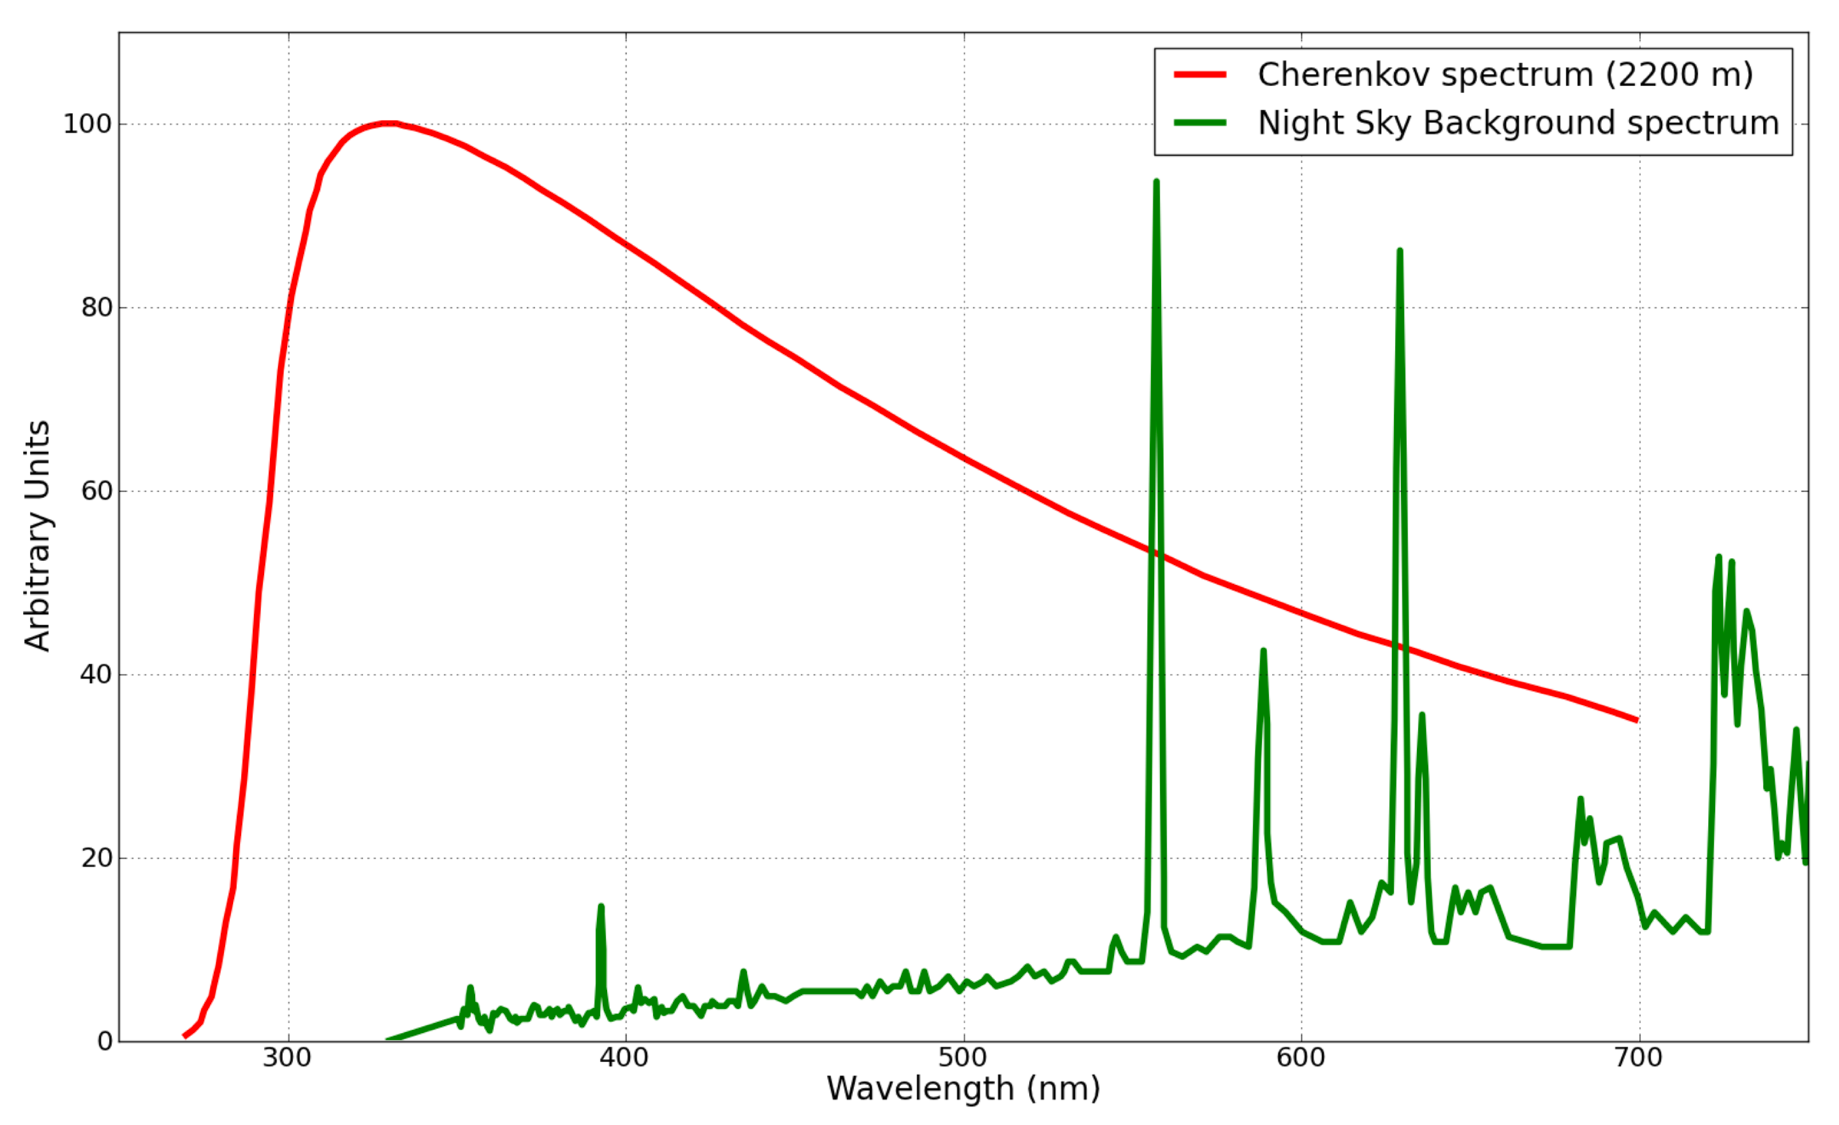
\includegraphics[width=\textwidth]{nsb} 
	\caption[Comparison of Cherenkov and NSB spectrum.]{Comparison of Cherenkov and NSB spectrum. The Cherenkov spectrum shown is expected at an altitude of \SI{2200}{m}. The NSB spectrum shown was measured at La Palma \cite{Bouvier2013}.}
	\label{fig:nsb}
\end{figure}

Two major background components need to be accounted for in \glspl{iact}:
\begin{description}
\item [Cosmic Ray Background] Protons (and heavier hadronic nuclei) are also capable of producing Cherenkov showers that are not entirely dissimilar to electromagnetic showers. As these particles are charged, they have been deflected by interstellar magnetic fields on their journey from their source, and therefore are not useful for \glspl{iact}. Therefore, these showers provide an isotropic background which is 1,000 times as numerous than the shower rate received from the discreet gamma-ray sources. However, a hadronic shower exhibits a morphology that is broader and less symmetric than that obtained from gamma-ray showers. Additionally, distinct features such as ``muon rings'', produced by highly penetrating muons reaching low altitudes such that the full Cherenkov cone is visible in a single telescope, accompany hadronic showers. Parametrisations of the Cherenkov shower image therefore enable the discrimination of the hadronic showers (see Chapter~\ref{ch6-reduction}. \change{images?}
\item [Night Sky Background] Due to the optical sensitivity of the cameras used by \glspl{iact}, the measurements taken are susceptible to starlight, moonlight, and artificial light pollution. The \gls{nsb} spectrum for La Palma, compared to the expected Cherenkov spectrum at an altitude of \SI{2200}{m}, is displayed in Figure~\ref{fig:nsb}. This background is excluded in two ways. Firstly, smart trigger logic and strict thresholds (such as the one described in Chapter~\ref{ch2-mechanics}) eliminate the triggering on \gls{nsb} photons. Secondly, unbiased charge extraction technique (described in Chapter~\ref{ch6-reduction}) exclude this noise from the signal.
\end{description}

The application of the \gls{iact} technique was first attempted in the 1960s, but the first large optical reflector built with the purpose of gamma-ray astronomy was the Whipple 10 m telescope in southern Arizona, 1968. At first, gamma-ray astronomy was polluted with unsubstantial claims of transient signals from a variety of pulsars and binaries, but these signals had marginal statistical significance \cite[][p.~9]{Weekes2003}. It wasn't until 20 years later, after further development of the technique, that the Crab Nebula was detected by Whipple in 1989, thus reigniting interest in the development of gamma-ray astronomy.

\begin{figure}
  \centering
  \begin{subfigure}[b]{0.35\textwidth}
  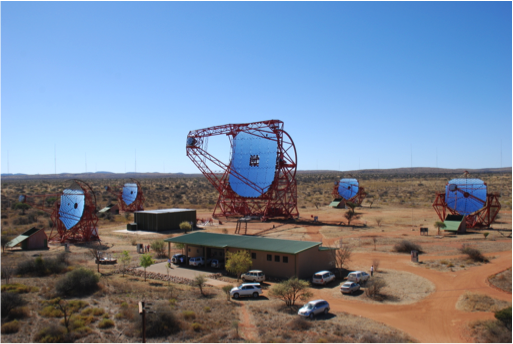
\includegraphics[width=\textwidth]{hess}
  \caption{H.E.S.S.}
  \label{fig:hess}
  \end{subfigure}
  ~
  \begin{subfigure}[b]{0.35\textwidth}
  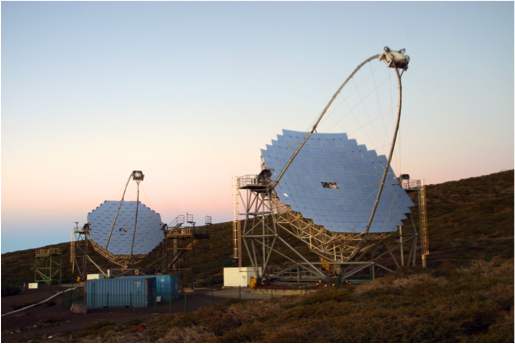
\includegraphics[width=\textwidth]{magic}
  \caption{MAGIC}
  \label{fig:magic}
  \end{subfigure}
  ~
  \begin{subfigure}[b]{0.45\textwidth}
  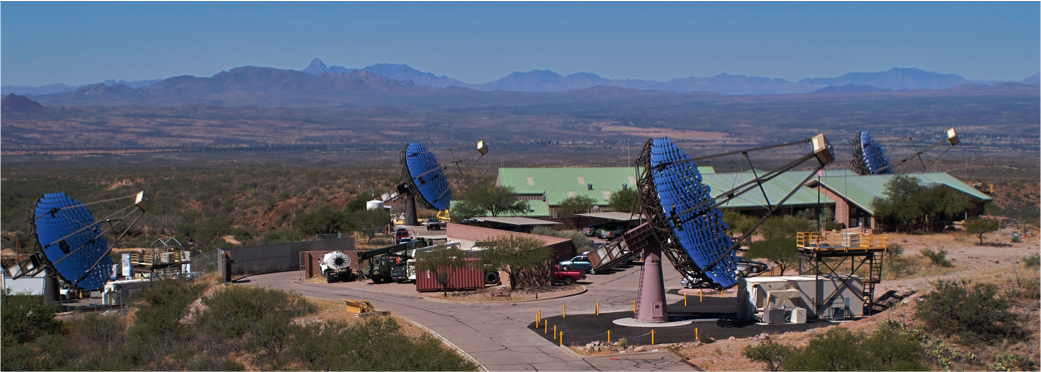
\includegraphics[width=\textwidth]{veritas}
  \caption{VERITAS}
  \label{fig:veritas}
  \end{subfigure}
  \caption{Photos of modern \glspl{iact}.}
  \label{fig:iacts}
\end{figure}

\begin{figure}
	\centering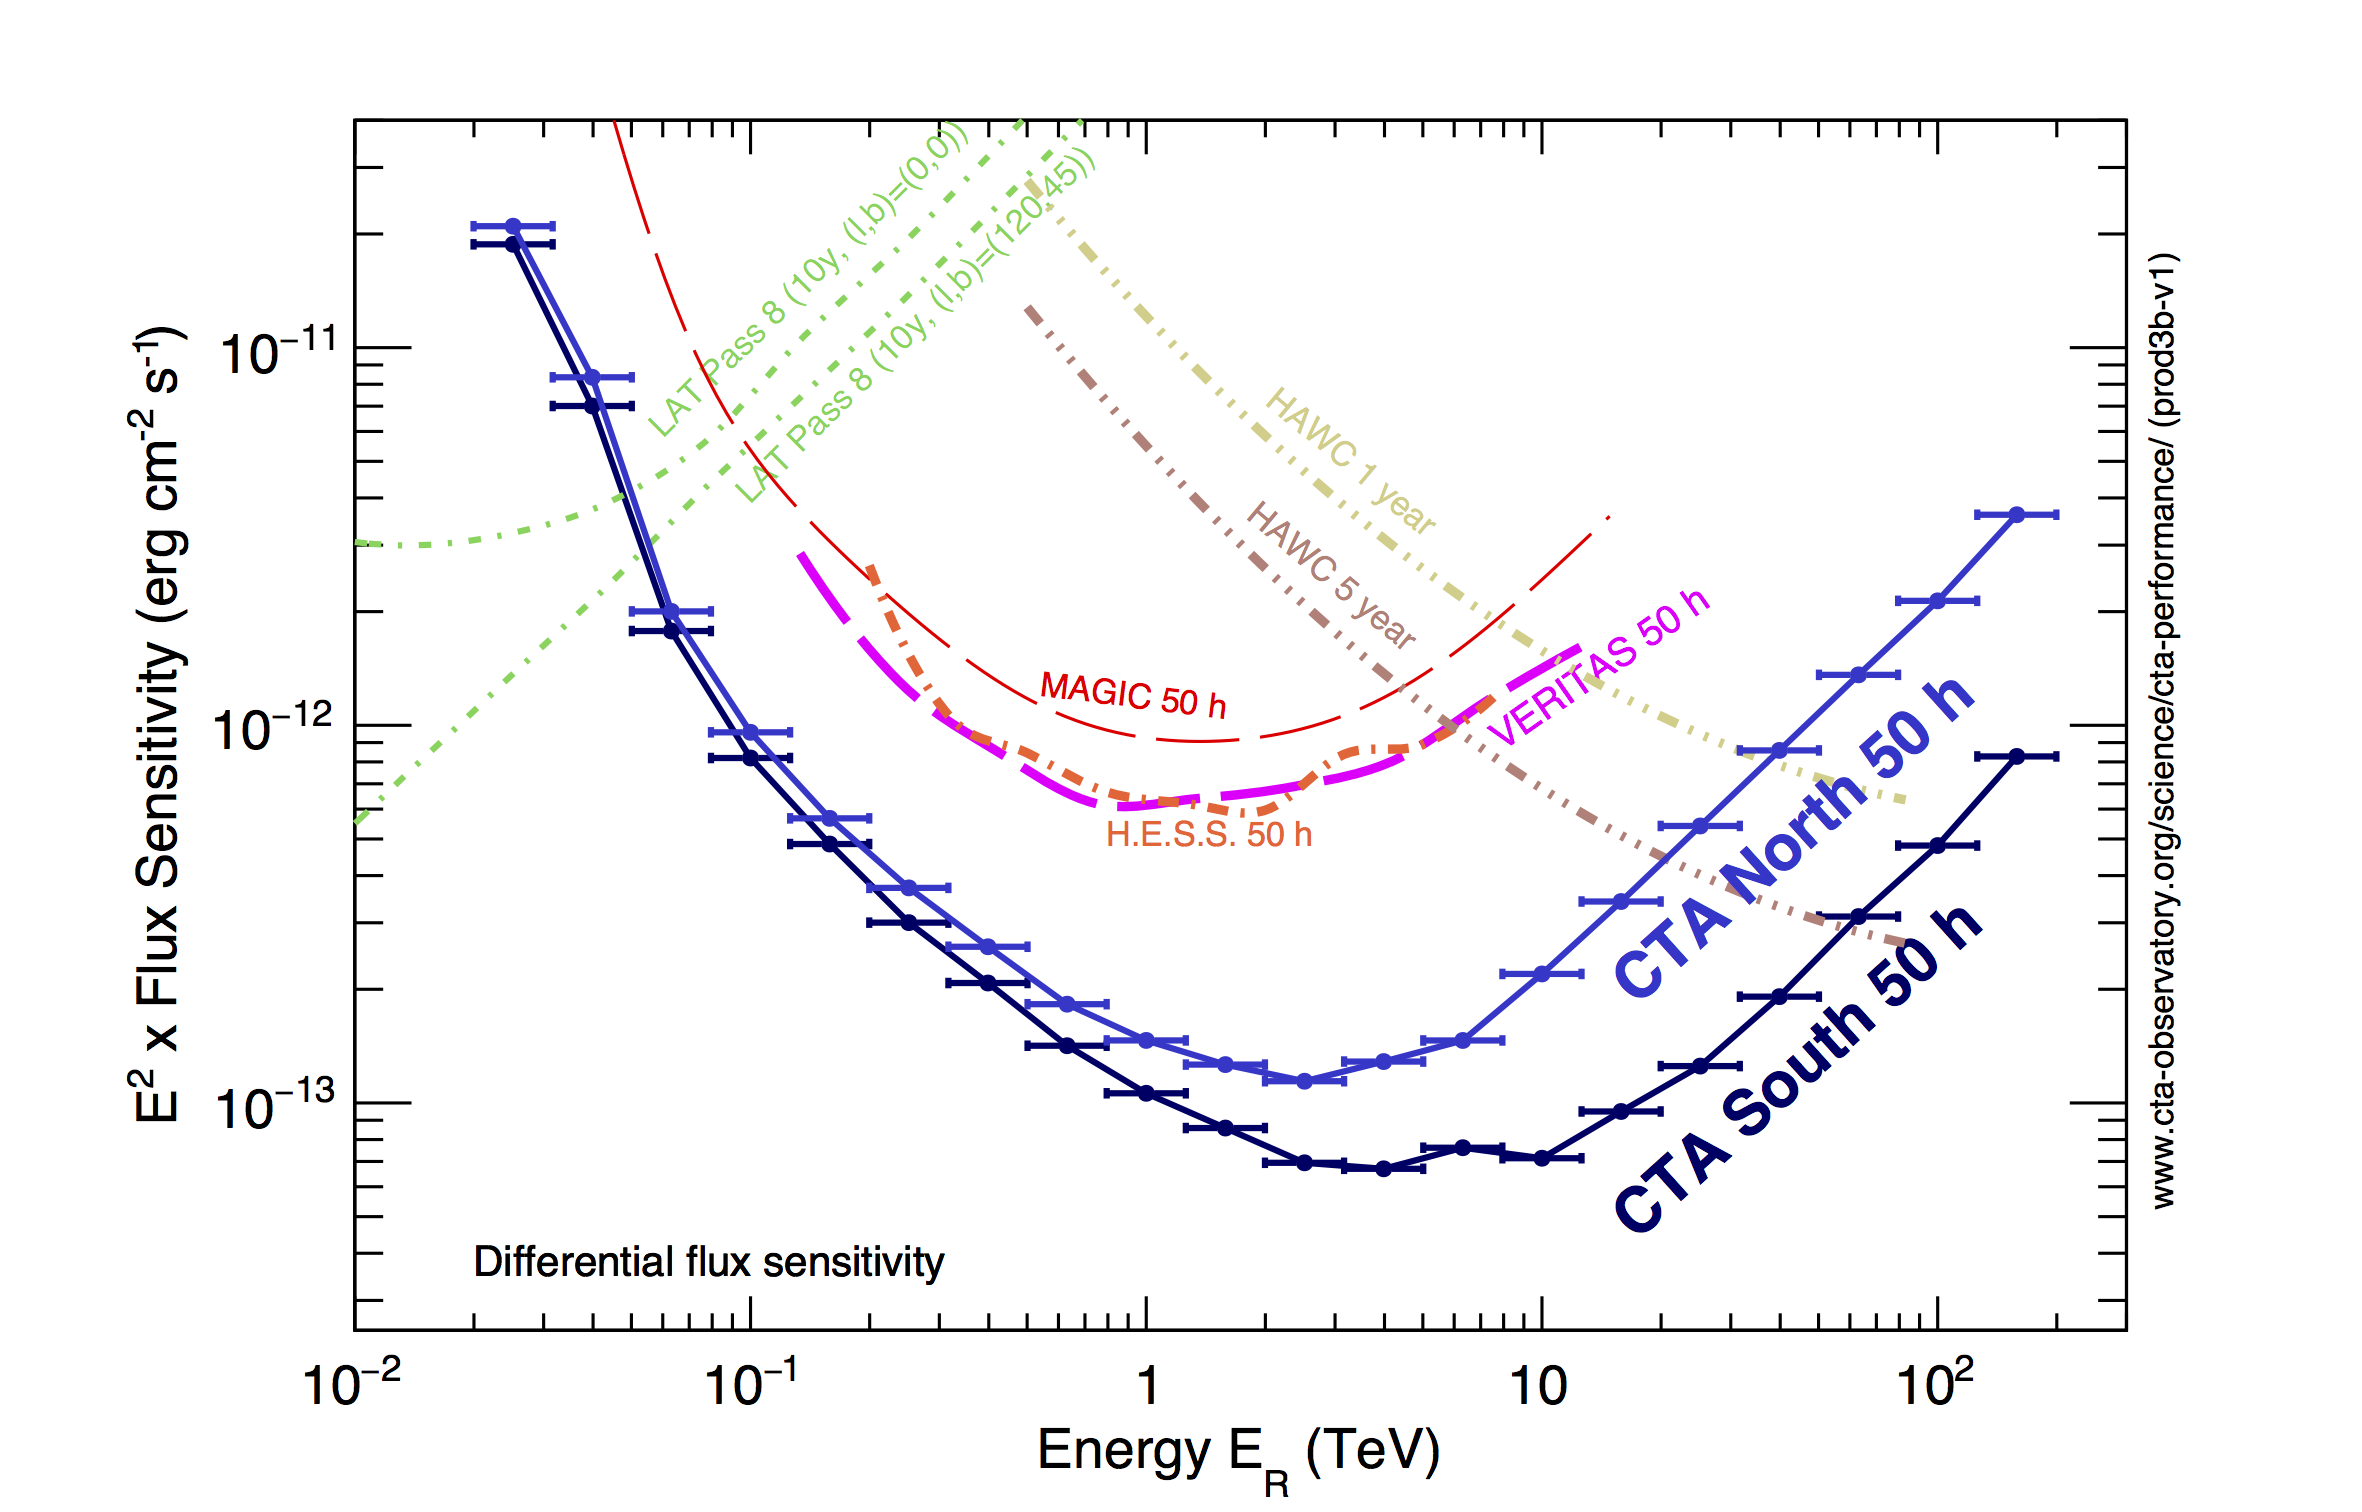
\includegraphics[width=\textwidth]{sensitivity} 
	\caption[Differential sensitivity of CTA.]{Differential sensitivity of CTA predicted by Monte Carlo simulations, compared to the performance of other gamma-ray instruments \cite{cta-performance}. The differential sensitivity has been defined as the minimum flux needed by CTA to obtain a 5-standard-deviation detection of a point-like source.}
	\label{fig:sensitivity}
\end{figure}

Modern \glspl{iact} include \gls{magic}, \gls{veritas}, and the most recent, \gls{hess} (Figure~\ref{fig:iacts}). All three of these telescope systems operate with the advantage of stereoscopic collaboration. In order to improve on the current \glspl{iact}, an array of ${\sim} 100$ telescopes was proposed, called the \gls{cta}. This array will have \cite{Acharya2013}:
\begin{itemize}
\item an improved sensitivity of 10 times over previous \glspl{iact} (Figure~\ref{fig:sensitivity}),
\item an observable gamma-ray energy range of \SI{30}{GeV} to \SI{100}{TeV},
\item a large (\SI{\sim 8}{\degree}) field of view for surveys,
\item improved angular and energy resolution,
\item and will be the first \gls{iact} to operate as an open observatory.
\end{itemize}

\section{The Cherenkov Telescope Array}

\begin{figure}
	\centering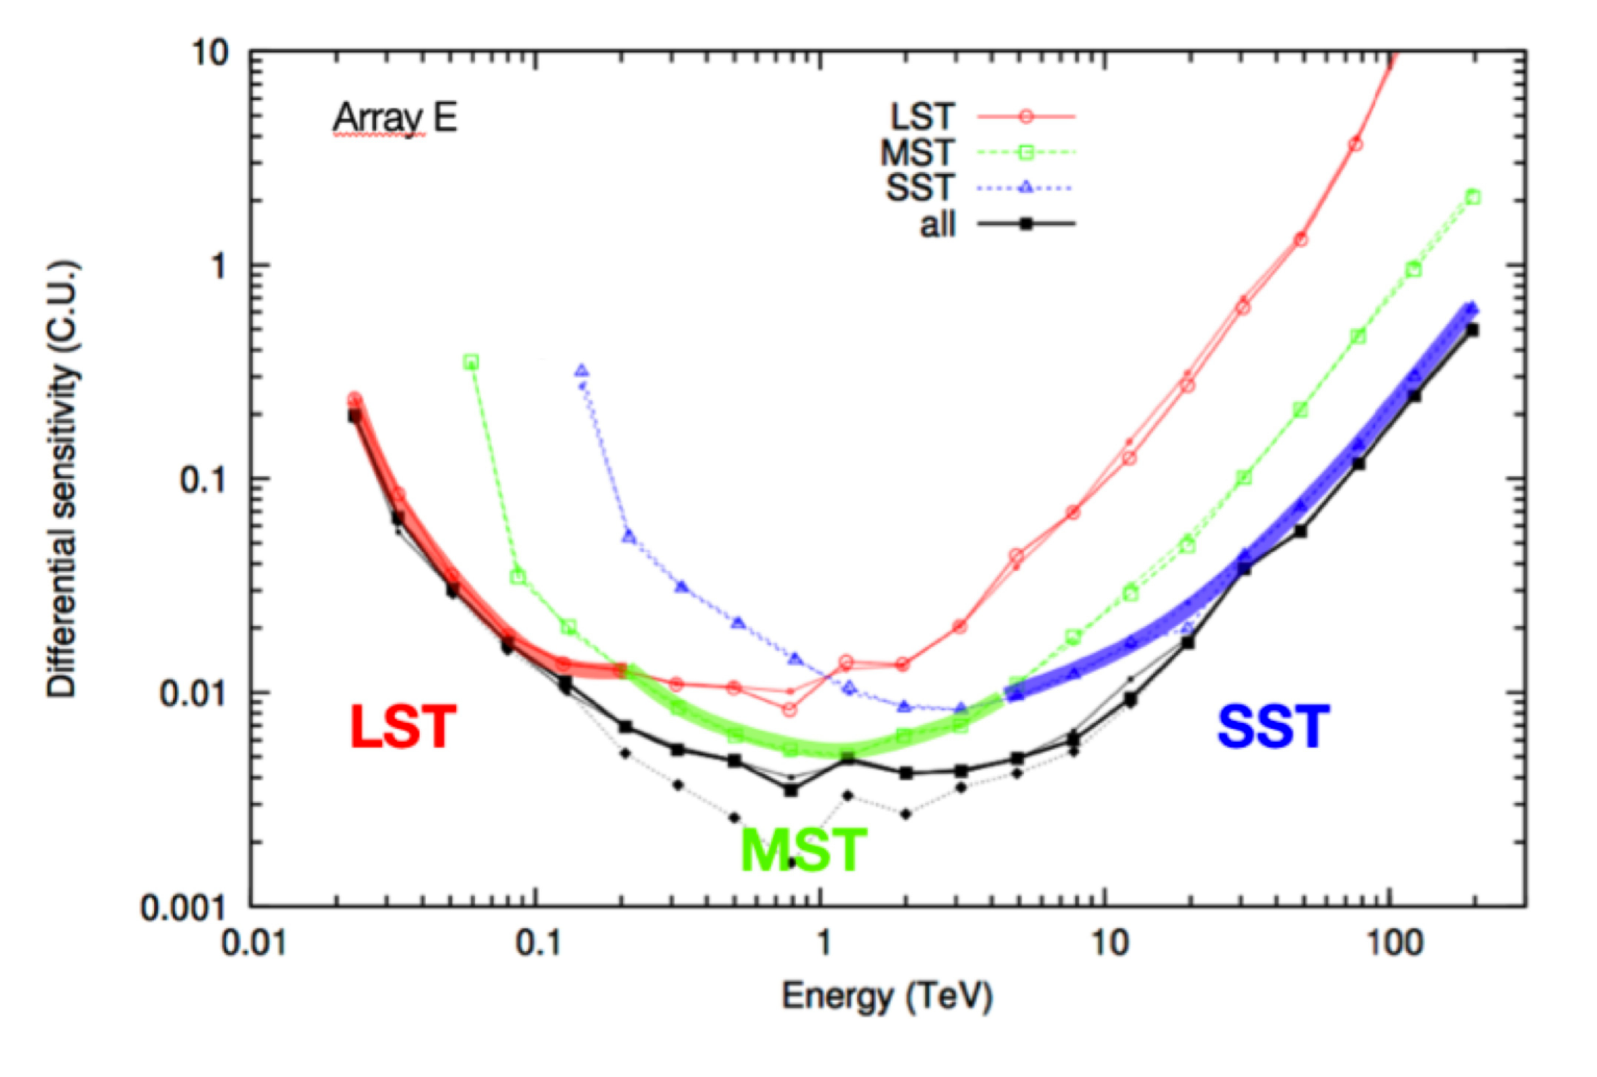
\includegraphics[width=\textwidth]{sensitivity_tel} 
	\caption[Differential sensitivity of the different CTA telescope types.]{Contribution of each telescope type within \gls{cta} to the total differential sensitivity \cite{Marano2014}.}
	\label{fig:sensitivity_tel}
\end{figure}

\gls{cta} will consist of three different sized telescopes:
\begin{itemize}
\item The \gls{lst}, with a mirror diameter of about \SI{23}{m} to enable the collection of as many photons as possible from the low energy showers (\SIrange{20}{150}{GeV}).
\item The \gls{mst}, covering the mid-range \SIrange{0.1}{10}{TeV} with mirror diameters of \SI{12}{m}.
\item The \gls{sst}, monitoring the high energies of \SIrange{1}{300}{TeV}, with mirror diameters of around \SI{4}{m}. Due to the rarity of higher energy showers, many \glspl{sst} need to be spread over an area of several square kilometres, to increase the chance of a detection \cite{Acharya2013}.
\end{itemize}
To illustrate these descriptions, the contributions of each telescope to the sensitivity of \gls{cta} is demonstrated in Figure~\ref{fig:sensitivity_tel}.

\begin{figure}
	\centering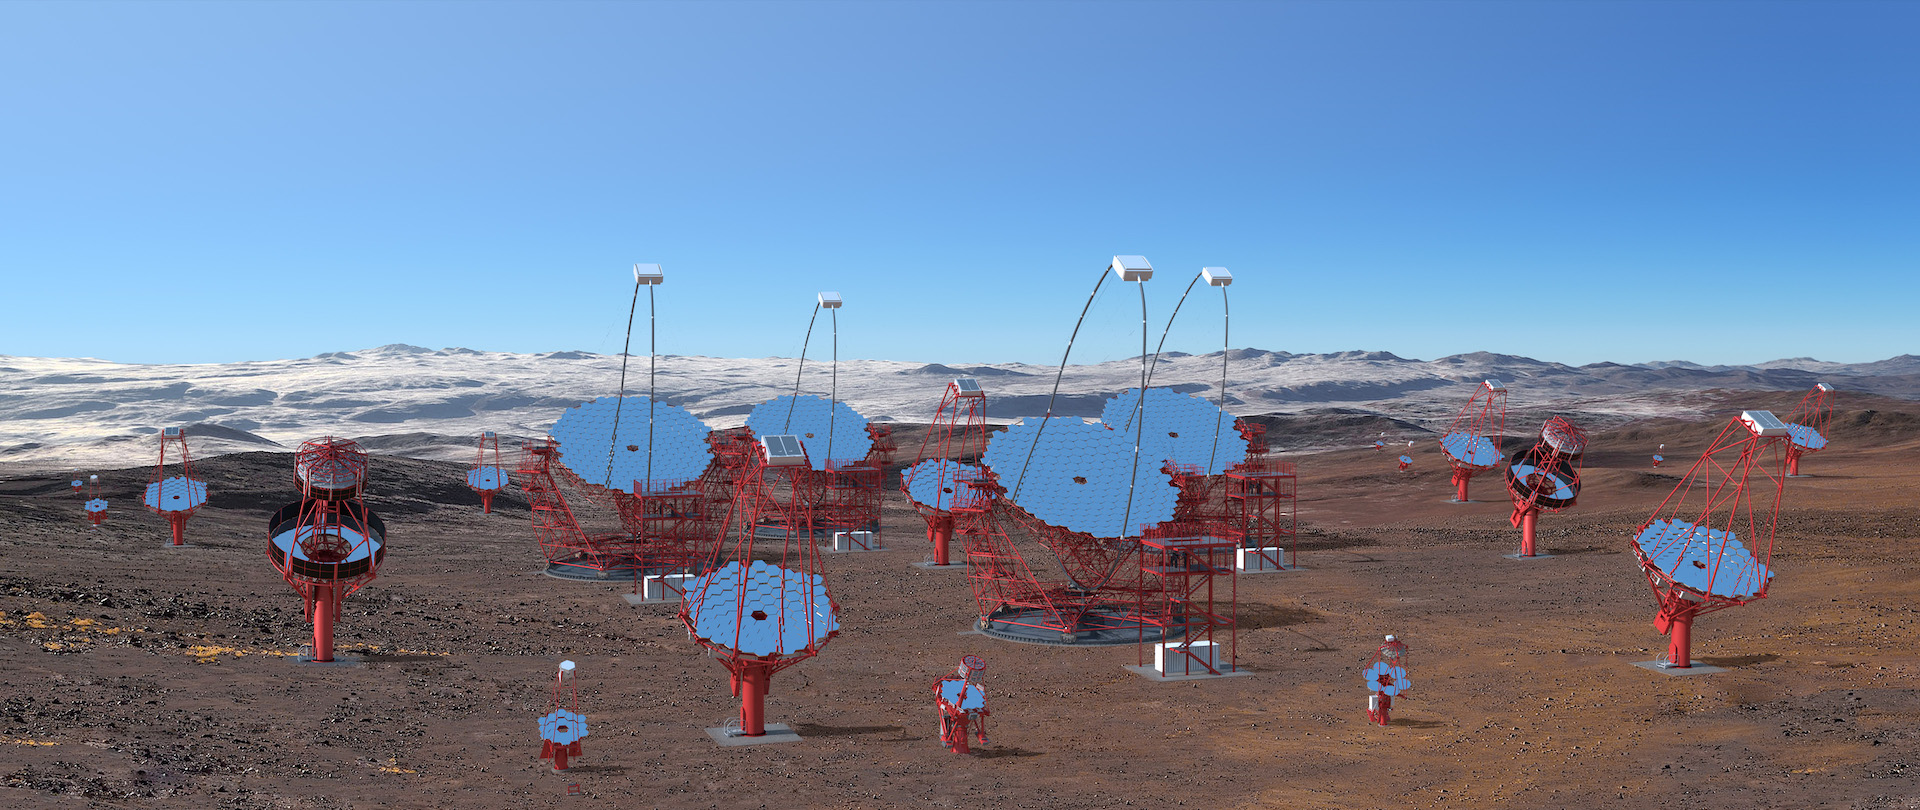
\includegraphics[width=\textwidth]{cta_south} 
	\caption[The southern-hemisphere Cherenkov Telescope Array.]{Computer-rendered graphic of the southern hemisphere site for the CTA three SST designs: GCT, ASTRI and SST-1M \cite{cta-sst}.}
	\label{fig:cta_south}
\end{figure}

Two \gls{cta} sites will exist. A northern hemisphere site for extragalactic observations will be built at La Palma, and is planned to contain 4 \glspl{lst} and 16 \glspl{mst}. As this site will focus on the energy range from \SI{20}{GeV} to \SI{20}{TeV}, no \glspl{sst} are included on the northern site. A southern hemisphere site will provide observations of the galactic plane, spanning the full energy range of \gls{cta}. Planned to be built nearby the Paranal Observatory in the Atacama Desert in Chile, the southern array is intended to feature 4 \glspl{lst}, 15 \glspl{mst}, and 70 \glspl{sst}, spread over \SI{4}{km \squared}. A visualisation of the \gls{cta} southern array is shown in Figure~\ref{fig:cta_south}.

\section{Small-Sized Telecopes}

\begin{figure}
	\centering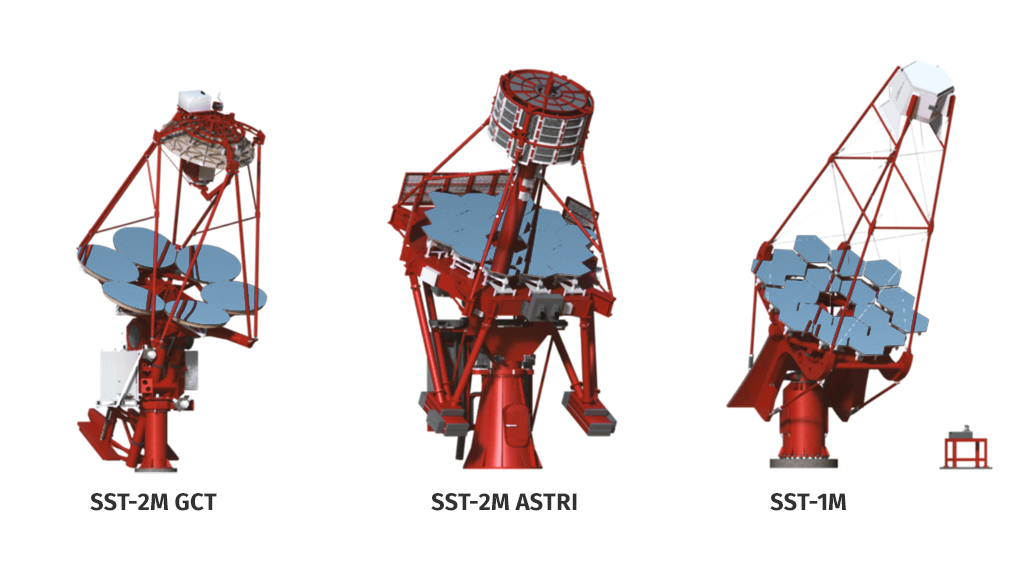
\includegraphics[width=\textwidth]{ssts} 
	\caption[The three SST designs.]{Computer-rendered graphics of the three SST designs: GCT, ASTRI and SST-1M \cite{cta-sst}.}
	\label{fig:ssts}
\end{figure}

Three designs for an \gls{sst} have been proposed:
\begin{itemize}
\item The SST-1M design, a single-mirror Davies-Cotton telescope developed in the colaboration between the Czech Republic, Ireland, Poland, Switzerland and Ukraine. The prototype structure was installed at the Institute of Nuclear Physics in Kraków, Poland in November 2013.
\item The \gls{astri} design features a dual-mirror Schwarzschild-Couder telescope structure. \gls{astri} is predominantly developed by Italy, however contributions were provided from Brazil and South Africa \cite{cta-sst}. The \gls{astri} prototype completed construction on Mt. Etna, Italy in 2014.
\item The \gls{gct} design also features a dual-mirror Schwarzschild-Couder telescope structure. \gls{gct} is being developed through collaboration between Australia, France, Germany, Japan, the Netherlands and the United Kingdom. The prototype telescope structure was inaugurated at the Observatoire de Paris-Meudon, France in November 2015. \gls{gct} is the telescope I have been associated with during my DPhil.
\end{itemize}
Visuals of all three telescopes are shown in Figure~\ref{fig:ssts}.

The Schwarzschild-Couder optical design was first proposed by German astrophysicist Karl Schwarzschild to eliminate optical aberrations across the \gls{fov}. This optical design has since gone through many interations, however it was never utilised for a reflector telescope due to the complexity and cost required to construct the mirrors \cite{Giro2017}. However, interest in the optical design was recently revitalised by \textcite{Vassiliev2007}, especially as it enables the utilisation of novel compact photosensors. Due to the same adoption of Schwarzschild-Couder optics, the telescopes of \gls{astri} and \gls{gct} have been specifically designed to accomodate the cameras from both \glspl{sst}. This increases the possibilities for the final \gls{sst} design for \gls{cta}.

\section{Science with the SSTs}

As shown in Figures~\ref{fig:sensitivity}~and~\ref{fig:sensitivity_tel}, the \glspl{sst} are responsible for exploring beyond the current energy frontier in gamma-ray astronomy. Within 50 hours, the \glspl{sst} will be able provide the same sensitivity as five years of observations with the \gls{hawc} observatory \cite{Consortium2018}. This enables \gls{cta} to provide insights into the most energetic processes in the universe, and address prevalant topics of debate in \gls{vhe} astronomy and particle phyiscs.

The high energy science cases of \gls{cta} are mostly concerned with the acceleration mechanisms that produce high energy cosmic rays. This has been an active topic of discussion in the past 100 years since their initial detection. It is therefore hoped that the \gls{cta} \glspl{sst} can provide new insights into these mechanisms. The different investigations related to this topic can be loosly consolidated into the following catagories:
\begin{description}
\item [Supernova Remnants] It is known that the galactic population of \glspl{snr} play an important role in the accelaration of cosmic rays to high energies. The detection of \si{TeV} photons from \glspl{snr} (suggesting an efficient acceleration mechanism), and the description of the diffusive shock acceleration mechanism, both corraborate with the detection of high-energy cosmic rays in the Earth's atmosphere \cite{Cristofari2017}. However, the detection of \si{TeV} photons from \glspl{snr} could instead be explained by the inverse-Compton scattering betweeen accelerated electrons and the ambient photon background. Therefore, the debate between a leptonic or hadronic origin is still ongoing \cite{Acharya2013}. While studies of individual \glspl{snr} have improved our understanding of the acceleration mechanisms, a population wide study may help constrain the parameters involved \cite{Cristofari2017}. The probe into higher energies with the \glspl{sst} will provide further information about the spectral energy distribution of the currently known \glspl{snr}, and the enhanced sensitivity of \gls{cta} will increase the population of \glspl{snr} known to emit at these energies.
\item [Origin of Cosmic Rays] Another important question regarding the locally measured flux of high-energy cosmic rays is their origin \cite{Bigongiari2016}. As just described, \glspl{snr} do appear to be a dominant source for these particles, but are they the only major contributor to the galactic cosmic rays? Expanding on the discovered \gls{vhe} galactic source population is the key to answering this question.
\item [Pevatrons] A further capability of \gls{cta} (provided by the \glspl{sst}) is the detection of extreme accelerators that power particles up to the \si{PeV} scale. As a result of the acceleration of hadronic cosmic rays to these energies, gamma rays with energies of /SI{100}{TeV} should be detectable from the accelerator. However, as the cross-section for inverse-Compton electron-photon interactions decreases very quickly above a few tens of \si{TeV} \cite{Consortium2018}, the absense of /SI{100}{TeV} gamma rays from these accelerators would suggest a leptonic origin. The identification of even one Pevatron acccelerator would therefore provide a huge breakthrough in the inevfffsfdstigtions into

and allow us to understand the physics of the most extreme accelerators in the Galaxy.

The preferential production of \SI{100}{TeV} photons by hadronic processes will be paramount in disentagling the ``problematic ambiguity between leptonic and hadronic origin'' of \gls{vhe} gamma rays \cite[][p. 132]{Consortium2018}.
\end{description}
%    \chapter{\label{ch2-mechanics}Camera Design \& Mechanics}

\minitoc

\notes[inline,caption={}]{
	\section{Plan}
	\subsection{Topics}
	\begin{itemize}
		\item Introduce TARGET architecture \& Wilkinson ADC
		\item Different TARGET versions
		\item FEE
		\item MAPMs
		\item SiPMS
		\begin{itemize}
			\item How they work
			\item Comparison investigations
			\item Property trade-offs
		\end{itemize}
		\item CHEC-M
		\item Changes for CHEC-S
		\item Future - MUSIC ASICs
	\end{itemize}
	\subsection{Questions}
	\begin{itemize}
		\item ?
	\end{itemize}
}

\section{Introduction}


\section{CHEC-M}

\change[inline]{schematic illustration of electronics}

\subsection{Multi-Anode Photomultiplier Tubes}

\subsection{Front-End Electronics}

\subsubsection{Pre-Amplifiers}

\subsubsection{TARGET}

\begin{figure}
	\centering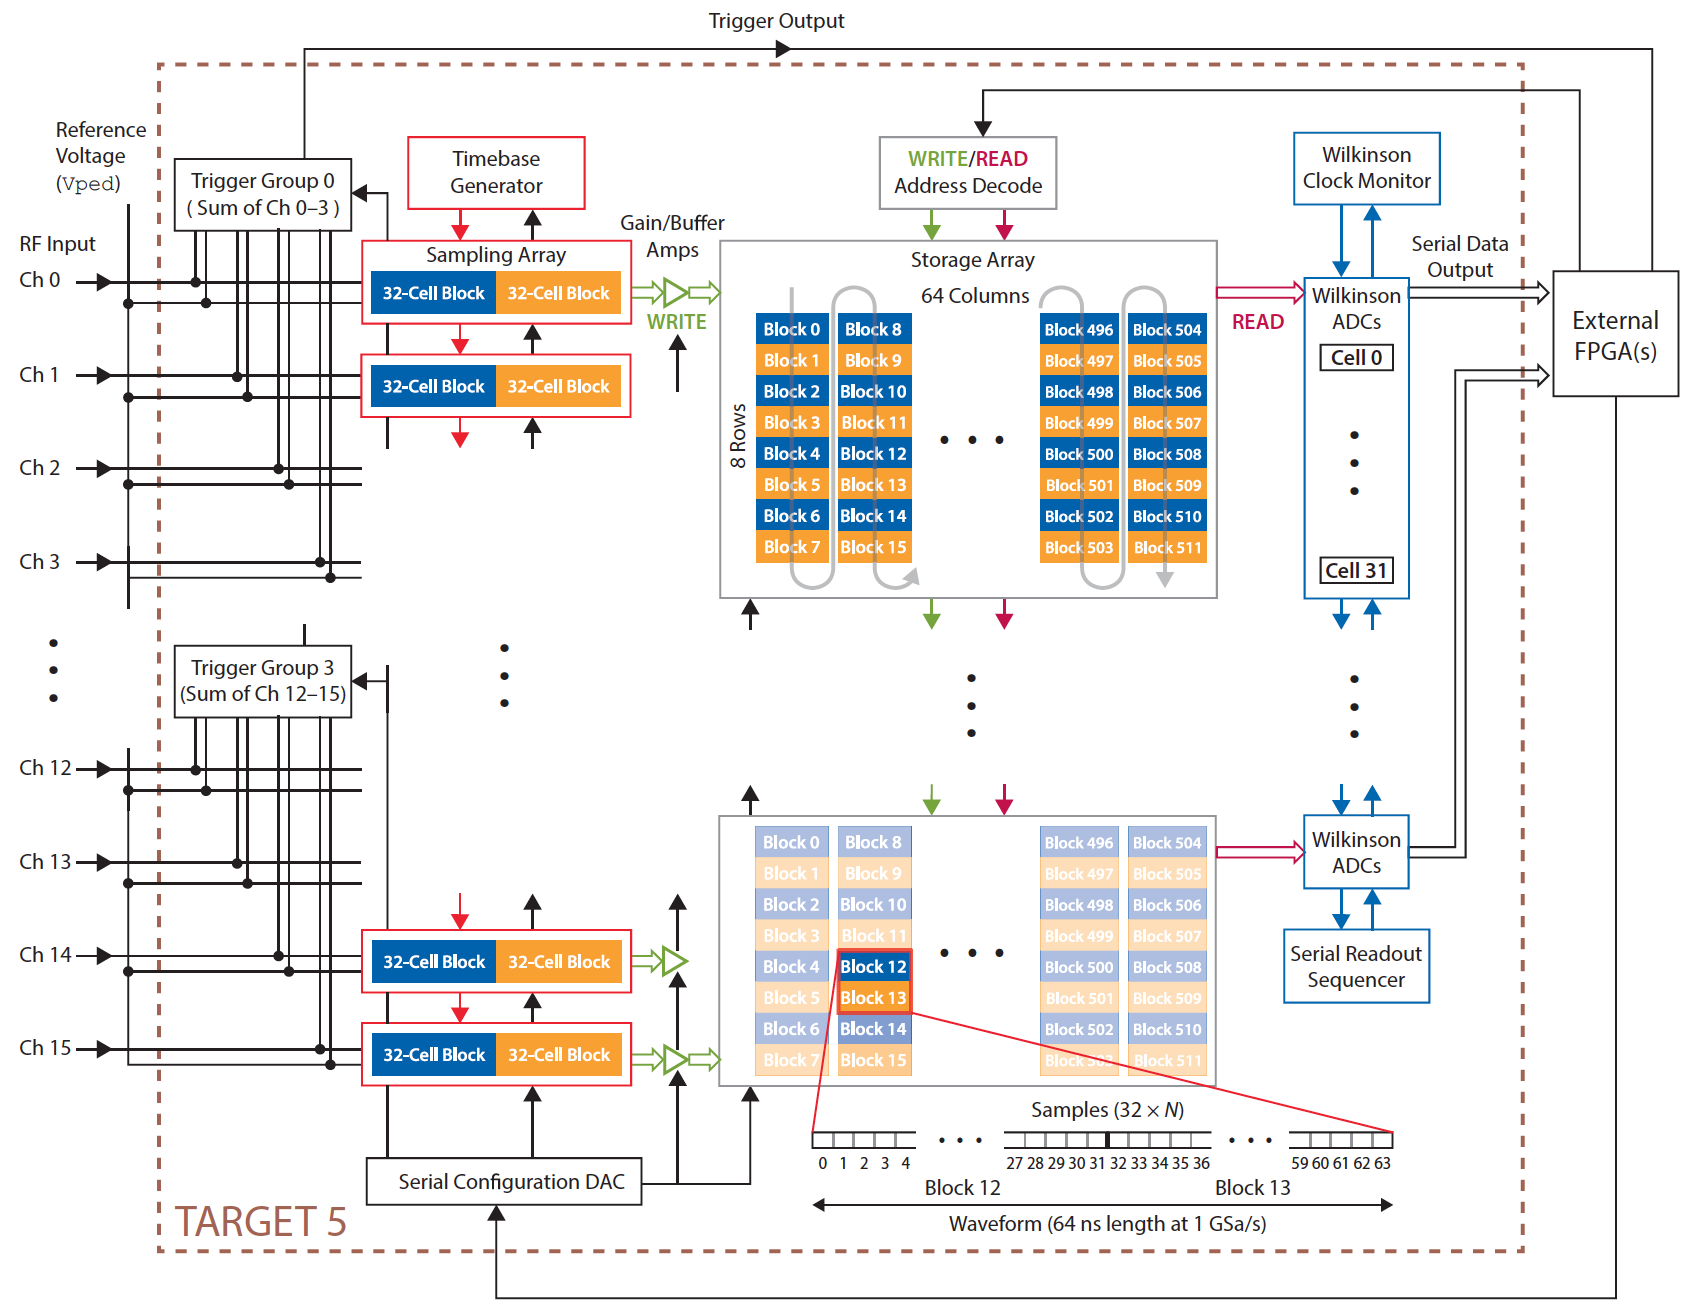
\includegraphics[width=\textwidth]{target5diagram} 
	\caption[Functional block diagram of the TARGET~5 ASIC.]{Functional block diagram of the TARGET~5 ASIC \cite{Albert2017} \change[inline]{Add more details}}
	\label{fig:target5diagram}
\end{figure}

\subsection{Back-End Electronics}

\subsubsection{Backplane}

\subsubsection{DACQ Boards}

\subsection{Peripherals\change{?}}

\subsubsection{LED Flashers}

\subsubsection{Chiller}

\section{CHEC-S}

\subsection{Silicon Photomultipliers}

\subsection{TARGET-C}

\change[inline]{larger dynamic range, reference tf plot????}

\change{name of TARGET-C FPGA?}

\section{Future}

\section{Lab Set-Up}

\section{Readout Characteristics}

\change{define ADC}
%    \chapter{\label{ch3-architecture}The CTA System Architecture} 

\minitoc

\section{Introduction}

Due to the large scope of \gls{cta}, in both its construction and operation, a formal approach towards a system architecture was adopted \cite{Dazzi2018}. One important aspect within this architecture is the distinction between the \gls{cta} Consortium and the \gls{cta} Observatory. The \gls{cta} Consortium is a group of scientists responsible for directing the science goals of the observatory, and for developing software and hardware (including cameras), which are supplied to the observatory as in-kind contributions. The Consortium consists of 200 institutes across 31 countries~\cite{cta-consortium}. Conversely, the CTA Observatory is the major astronomical facility that acquires the science data and delivers them to a wide user community as an open observatory. The \gls{cta} Observatory gGmbH is the legal entity for \gls{cta} in the preparation for the implementation of the \gls{cta} Observatory, and works in close cooperation with the Consortium during this process \cite{cta-observatory}.

The purpose of the \gls{cta} Architecture is to ensure a coherent view of the functionality and capabilities of \gls{cta}. The \gls{cta} Architecture can then drive the pre-construction phase to guarantee:
\begin{itemize}
\item a coherent development process,
\item the seamless integration of the developed units into the final array,
\item and that the performance of the final array is capable of meeting its science goals.
\end{itemize}
In this chapter, I describe two concepts connected to the \gls{cta} Architecture that are important in the context of this thesis. Firstly, the \gls{cta} requirements which all cameras, including \gls{chec}, must meet. Secondly, the descriptions of how data are handled in \gls{cta}, including the data flow and data level definitions.

\section{Requirements}

In order to ensure the science goals of \gls{cta} are achievable, and that the observatory remains operational for the full 30 year life-time, certain standards must be upheld by all components of the observatory; this is the purpose of the \gls{cta} requirements. The requirements cover every aspect of the observatory, including: the survival and operation under different environmental conditions (e.g.\@ \requirementref{B-ENV-1120 Earthquake collapse prevention (South)}, \requirementref{B-ENV-0320 Survival humidity}), the time allowed by the analysis pipeline for processing (e.g.\@ \requirementref{A-OBS-0810 Data Processing Efficiency}), the reliability of telescope components (e.g.\@ \requirementref{B-TEL-0520 Structure Lifetime}), and the ability to meet the expected performance under different observation conditions (e.g.\@ \requirementref{PROG-0025 Differential Sensitivity under Low Moonlight - North}). In order for an in-kind contribution to be accepted, it must meet the requirements defined by the observatory. These requirements are therefore the standards against which we assess the performance of \gls{chec}, and are the primary drivers in my development of the low-level calibration and analysis. However, there exist more than 60 requirements specifically tailored to the cameras. Consequently, the full review of the camera is a large undertaking that extends beyond the scope of this thesis. Here, only the requirements that have relevance to the topics of this thesis are discussed.

It is important to note that the requirements, located on the \gls{cta} Jama website~\cite{cta-jama}, are currently under review and therefore subject to change. A major change that was under way at the time of this writing was the redefinition from units of photoelectrons to photons. Originally, a common consolidated \gls{pmt} was envisioned for all cameras in \gls{cta}, motivating the expression of relevant requirements in terms of photoelectrons. However, due to the advances in sensor technology and the adoption of \glspl{sipmt} by cameras such as \gls{chec-s}, this assumption has led to problems with such a definition \cite{petophotons}. While one camera would measure X photoelectrons for a particular number of photons, a different camera (with a different \gls{pde}) would measure Y photoelectrons. Additionally, the definition of the requirements in photoelectrons encourages the cameras to be optimised in terms of their \gls{enf}, potentially at the cost of its \gls{pde}. The measurement in photons is therefore a much more coherent expression of signal for the array, which ensures requirements are stated in terms of the cameras ability to detect the Cherenkov-shower photons, instead of the cameras ability to resolve the number of photoelectrons generated in the photosensor. 

As the procedure of converting the requirements from photoelectrons to photons is ongoing, this thesis will contain reference to the photoelectron definition of the requirements. A copy of the requirements relevant to this thesis, in the form they exist in Jama at the time of this writing, are included alongside the discussion in this section. This is to ensure clarity about which version of the requirement definition is being referred to. Future investigations should check the latest requirement definition. \vfill

\subsection{B-TEL-1010 Charge Resolution} \label{section:cr}

\begin{requirement}{Jama Excerpt} 
	The required fractional charge resolution for Cherenkov signals in each Camera pixel for a specified background level of 0.125 photoelectrons/ns is given in the Figure below and Table attached. Charge measurements must be possible for 0-1000 photoelectron signals. The average charge resolution should be calculated for the reference Gamma-Ray Spectrum.
    
	\centering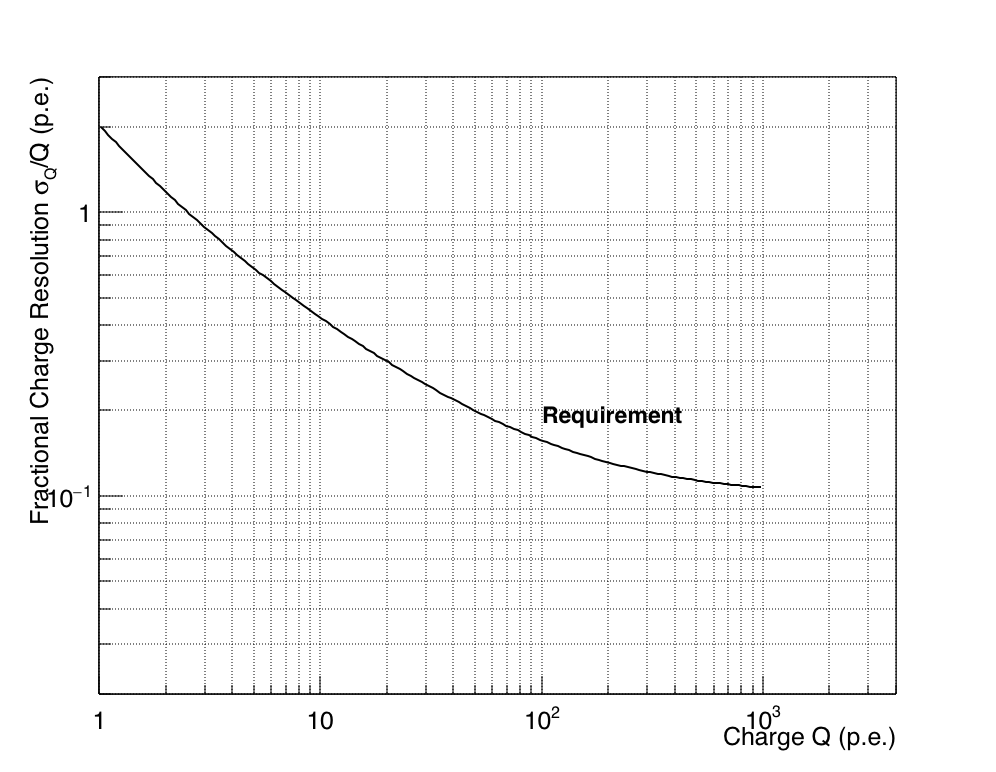
\includegraphics[width=0.8\linewidth]{charge_res_req}
	\captionof{figure}[Charge resolution requirement.]{Fractional rms charge resolution $\sigma_Q/Q$ per pixel for different Cherenkov light signal amplitudes, expressed in units of photoelectrons (p.e.). All sources of fluctuations, including Poisson fluctuations in photoelectron number, must be included. The true pixel charge $Q$ is that measured in an ideal detector with the same photon-detection efficiency. }\label{fig:charge_res_req}
    
\begin{itemize}
\item [Notes:] It is expected that this requirement is verified with reference to:

- Monte Carlo simulation of Cherenkov light from gamma-ray initiated showers (using a verified telescope model),

- Level-C Specification on Laboratory Measured \textit{Charge Resolution},

- Monte Carlo simulation of the laboratory test set-up (as a means of telescope model verification).

Note that between \SI{1000}{\pe} and \SI{2000}{\pe}, some sensitivity to increasing input signal must exist. \newline
This requirement applies to post-calibration (DL1) data. \newline
Note that this requirement will likely need to be expanded to cover performance at higher NSB levels.
\end{itemize}
\end{requirement}

\subsubsection{Definition}

The standard criterion for the low-level camera performance used in \gls{cta} is the \textit{Charge Resolution}. It encompasses both the bias and the standard deviation of the extracted charge versus the expected charge to provide a measure of the waveform, calibration, and charge reconstruction quality. Analogous to the Root-Mean-Square Error, the fractional \textit{Charge Resolution} $\frac{\sigma_Q}{Q_T}$ for a particular ``true charge'' $Q_T$ (the number of photoelectrons that were produced in the sensor, before multiplication) is defined as:
\begin{equation} \label{eq:charge_res}
\frac{\sigma_Q}{Q_T} = \frac{1}{Q_T} \sqrt{\frac{\sum_{i=0}^N (Q_{M_i} - Q_T)^2}{N}},
\end{equation}
where $N$ is the total number of measured charges, $Q_{M_i}$, with that value of $Q_T$. The associated \gls{cta} requirement defines the maximum allowed values of $\frac{\sigma_Q}{Q_T}$ for values of $Q_T$ between \SIrange{1}{1000}{\pe}, which must be adhered to when resolving the signal for any camera in \gls{cta}.

\subsubsection{Requirement Derivation}

The uncertainty in charge reconstruction can be expressed in the form:
\begin{equation} \label{eq:charge_res_req}
\frac{\sigma_Q}{Q} = \frac{1}{Q} \sqrt{\sigma_0^2 + \sigma_{ENF}^2 Q + \sigma_G^2 Q^2},
\end{equation}
where $\sigma_0$ encapsulates the noise contributions (electronic and \glsb{nsb}), $\sigma_{ENF}$ is the \textit{Excess Noise Factor} (a measure of fluctuations in charge amplification, see Section~\ref{section:enf}), and $\sigma_G$ is the multiplicative errors in the calibration (i.e.\@ the miscalibration) of the gain \cite{petophotons}\cite{Ohm2012}. $\sigma_0$ can be further expanded in terms of the two primary noise contributions:
\begin{equation} \label{eq:charge_res_nsb}
\sigma_0 = \sqrt{\mathit{NSB} \times t_w + n_e^2},
\end{equation}
i.e.\@ the $\mathit{NSB}$ rate (which includes the \gls{dcr} for the purpose of this discussion) is coupled with the effective signal readout window size, $t_w = \SI{15}{ns}$, and summed with the electronic noise, $n_e$. A contribution from electronic noise of $n_e = \SI{0.87}{\pe}$ is assumed, combined with a value of $\mathit{NSB} = \SI{0.125}{\pe/ns}$ as defined in the requirement. A value of $\sigma_G = 0.1$ and $\sigma_{ENF} = 1.2$ is also assumed \cite{petophotons}. The resulting combination of miscalibration and noise factors in Equation~\ref{eq:charge_res_req} gives the \textit{Charge Resolution} requirement illustrated in Figure~\ref{fig:charge_res_req}.

\subsubsection{Approach}
As it is impossible to know the ``true charge'' generated by a Cherenkov signal in the field, Monte Carlo simulations must be relied upon in order to prove a camera meets this requirement. The process for achieving this is outlined in the notes to the requirement. It is expected that this requirement is validated in three ways:
\begin{enumerate}
\item With lab measurements where the camera is uniformly illuminated with a calibrated light source.
\item With simulations of the previous approach, in order to verify the simulation model of the camera.
\item With Monte Carlo simulations of Cherenkov signals incident on the full telescope model.
\end{enumerate}
The final item is the most important in confirming the requirements are met, as temporally-uniform illuminations do not sufficiently test the ability to find the signal pulse in the waveforms for the case of a Cherenkov-shower illumination. The prior items are important to verify that the \textit{Charge Resolution} result obtained in the final item is applicable to the real camera, i.e.\@ the simulation model of the camera is accurate.

The simulation package \pkg{sim\_telarray} (Chapter~\ref{ch4-software}) stores the ``true charge'' generated in the photosensor for each shower event into an output file. Therefore, with an accurate simulation model of the camera, it is an appropriate package for investigating a camera's performance against this requirement. However, in order to ensure Poisson fluctuations in photoelectron number are included, as per the requirement, when using the ``true charge'' stored in the simulation file, the corrected form of Equation~\ref{eq:charge_res} is
\begin{equation} \label{eq:charge_res2}
\frac{\sigma_Q}{Q_T} = \frac{1}{Q_T} \sqrt{\frac{\sum_{i=0}^N (Q_{M_i} - Q_T)^2}{N} + Q_T}.
\end{equation}
With the form in Equation~\ref{eq:charge_res2}, a perfect detector that consistently reads-out a ``measured charge'' with an equal value to the ``true charge'' would hit the Poisson limit. This limit ensures realistic conclusions can be reached from the Monte Carlo simulations, as it is not physically possible to know the ``true charge'' generated inside the photosensor, free from fluctuations.

\subsection{B-TEL-1030 Time Resolution} \label{section:time_res}

\begin{requirement}{Jama Excerpt} 
The rms difference in the reconstructed signal arrival time for any two simultaneously illuminated pixels in the Camera with amplitudes of five photoelectrons must not exceed 2 ns. This is for a specified background level of 0.125 photoelectrons/ns.

\begin{itemize}
\item [Notes:] This requirement should be verified based on laboratory testing of a prototype at the specified background level.
\end{itemize}
\end{requirement}

A second important requirement concerning the signal inside the waveforms is the \textit{Time Resolution} requirement. While the capability to accurately locate the signal is already assessed by the \textit{Charge Resolution}, the purpose of this requirement is to instead ensure that the physical camera exhibits sensible behaviour with regards to the relative location of the signal between pixels, per event. One interpretation of the \textit{Time Resolution} $\sigma_T$ is the standard deviation of the difference in pulse time between every pixel in the camera, per event. This can be expressed as:
\begin{equation} \label{eq:time_res}
\sigma_T = \sqrt{\frac{\sum_{i=0}^N(\sum_{j=i+1}^N (T_{i-j} - \average{T}_{i-j})^2)}{\binom{N}{2} - 1}},
\end{equation}
\begin{equation} \label{eq:time_res2}
\average{T}_{i-j} = \frac{\sum_{i=0}^N(\sum_{j=i+1}^N T_{i-j})}{\binom{N}{2}},
\end{equation}
where $T_{i-j} = T_i - T_j$, i.e. the difference between the extracted pulse time $T_i$ for pixel $i$, and extracted pulse time $T_j$ for pixel $j$. $\binom{N}{2}$ is the binomial coefficient of the number of pixels $N$ ``choose'' 2, i.e.\@ the total number of unique pixel combinations.

In this definition of \textit{Time Resolution}, $\sigma_T$ is calculated per event. However, the camera is better characterised by the mean and standard deviation of $\sigma_T$ over multiple events. In order to meet the requirement, the \textit{Time Resolution} should be under \SI{2}{ns} for pixels with measured charges above \SI{5}{\pe}, in an environment containing an \gls{nsb} photon rate of at least \SI{0.125}{\pe/ns}. Any pixel timing corrections (described later in Section~\ref{section:timing_corrections}) that are required should be applied to the pulse time extracted from the waveform. Furthermore, the \textit{Time Resolution} does not need to be extracted with the same approach as used in the charge extraction, as long as the approach is justifiable.

\subsection{B-TEL-1295 Pixel Availability} \label{section:pixel_availability}

\begin{requirement}{Jama Excerpt}
During observations, at least 95\% of all camera pixels must be available and usable for data analysis. In addition, continuous regions of non-functioning pixels must not exceed 2\% of all camera pixels. Pixels excluded due to NSB levels beyond those required are not included in this budget.
\end{requirement}

This requirement sets a limit on the amount of ``dead'' pixels that a camera is allowed to have before the entire camera is considered to be unavailable. For \gls{chec}, which contains 2048 pixels, this imposes the following possible limitations:
\begin{itemize}
\item The camera may only have a maximum of 102 dead pixels. This allows 3 dead pixels per module.
\item The amount of contiguous pixels that are allowed to be dead is 41, therefore if an entire \gls{target} module dies (each module containing 64 pixels), the camera's capabilities become insufficient for the \gls{cta} requirements. However, a maximum of two \gls{target} \glspl{asic} (each \gls{asic} containing 16 pixels) are allowed to die.
\end{itemize}

\begin{figure}
 	\centering
  	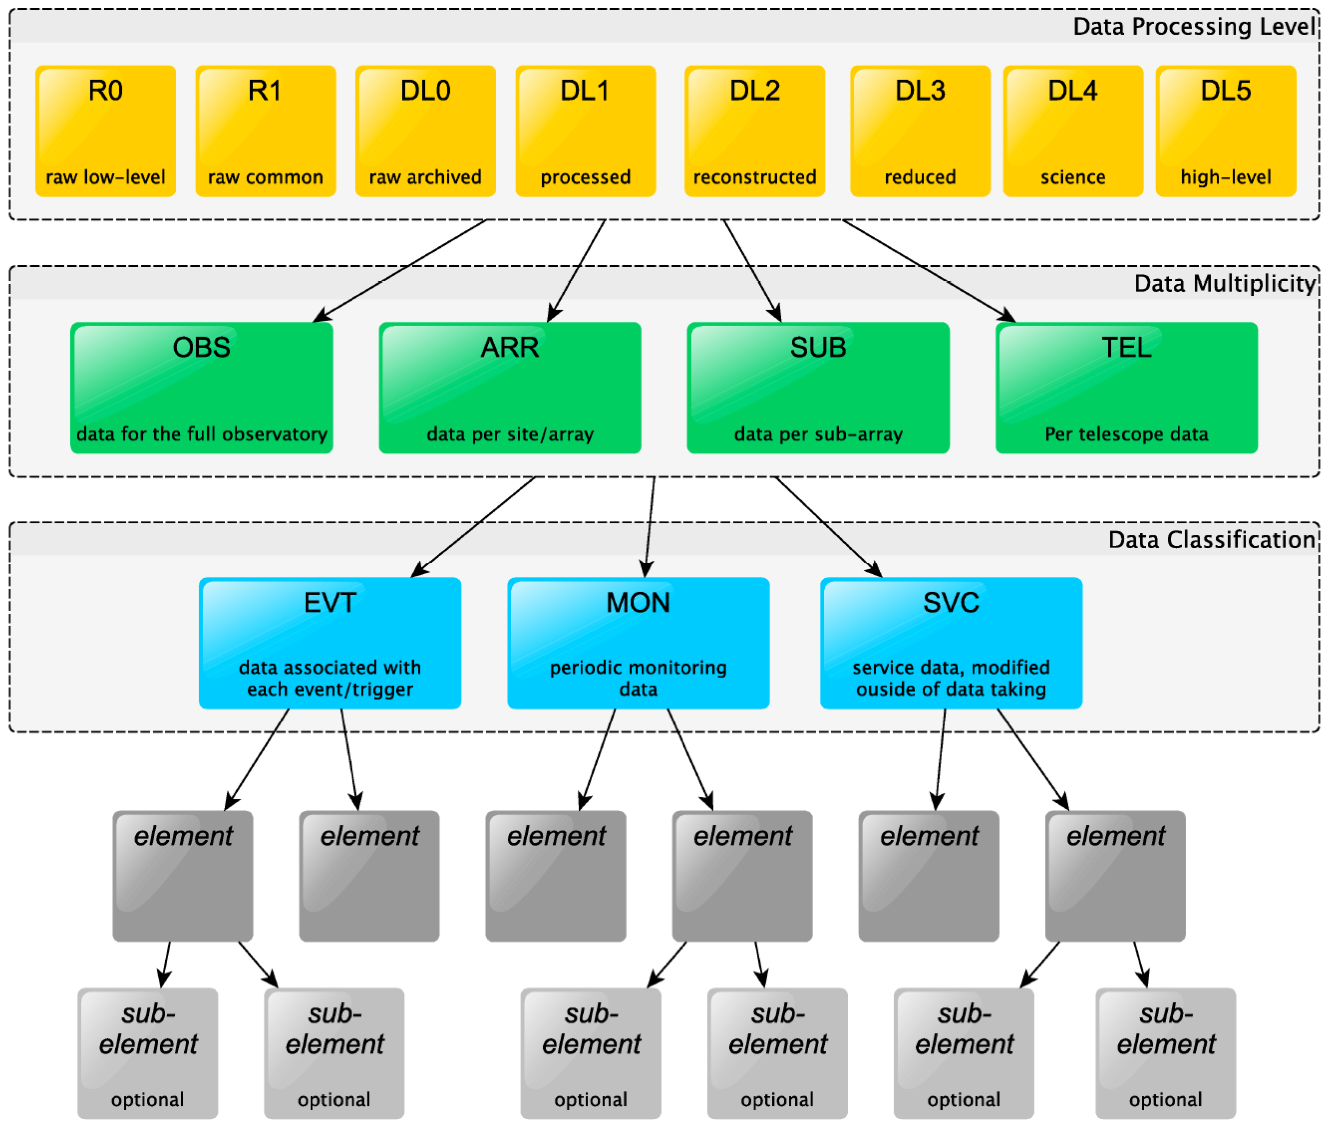
\includegraphics[width=\textwidth]{high_level_data_model} 
	\caption[High-level data model hierarchy.]{Hierarchy of data element names including the data level, the classifications of data (based on their rate), and data elements/groups and sub-elements/groups \cite{Kosack2017}.}
	\label{fig:high_level_data_model}
\end{figure}

\begin{figure}
 	\centering
  	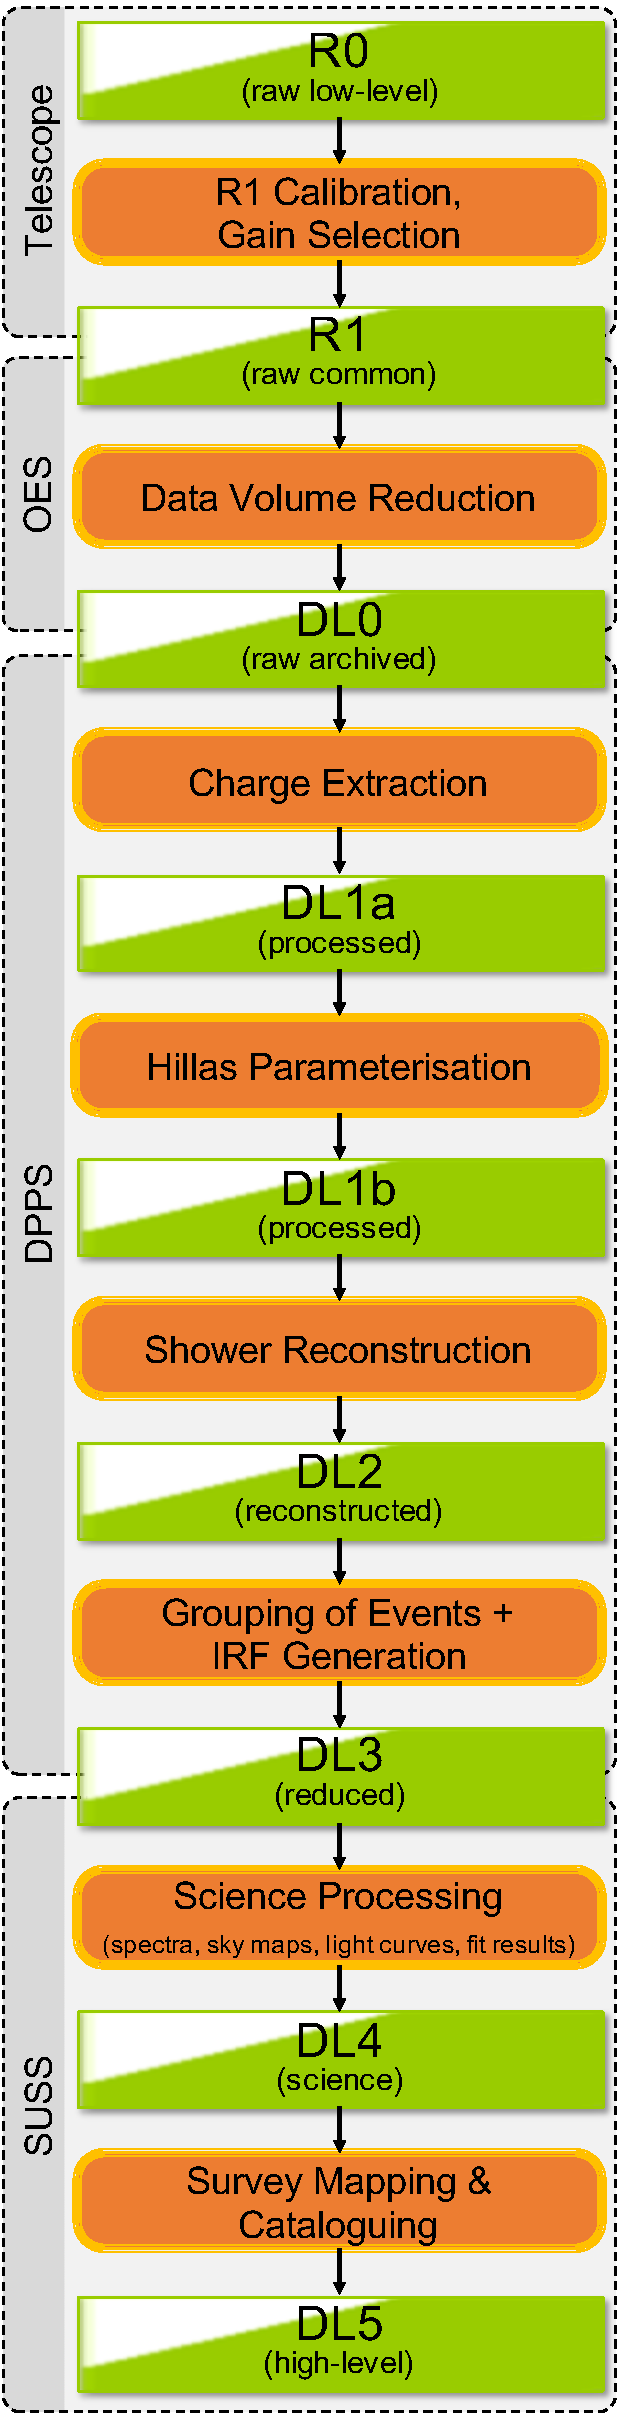
\includegraphics[height=0.9\textheight]{dataflow} 
	\caption[Simplified camera data flow.]{Simplified camera data flow, showing the \textit{EVT}-classified data streams (in green) and the processing steps between them (orange). The levels are grouped by the systems responsible for them.}
	\label{fig:dataflow}
\end{figure}


% \begin{wrapfigure}[37]{r}{0.32\textwidth}
% 	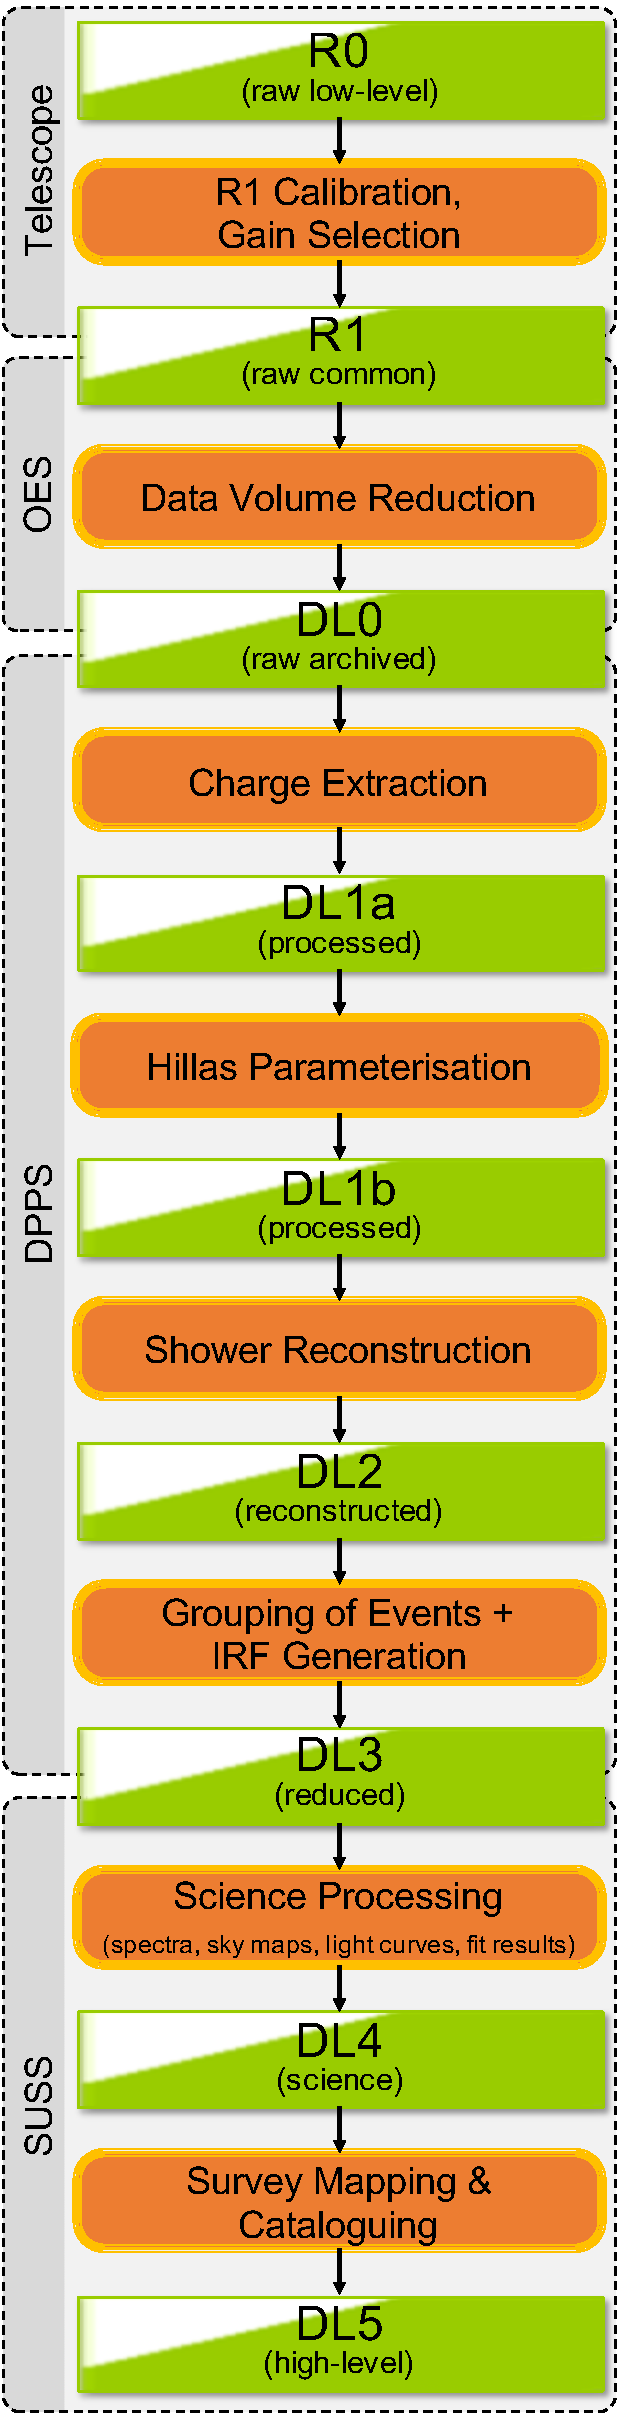
\includegraphics[width=0.32\textwidth]{dataflow}
% 	\caption[Simplified camera data flow.]{Simplified camera data flow, showing the \textit{EVT}-classified data streams (in green) and the processing steps between them (orange). The levels are grouped by the systems responsible for them.}
% 	\label{fig:dataflow}
% \end{wrapfigure}

\section{Data Level and Flow Model} \label{section:data_levels}

Further aspects of the \gls{cta} Architecture that are relevant to this work are the \textit{Data Processing Level} definitions, and the flow between them. These definitions dictate how the data obtained from the telescopes are handled within the observatory, and are important in ensuring each telescope adopts a similar processing chain to guarantee compatibility between themselves and the pipeline framework software. Figure~\ref{fig:high_level_data_model} shows the full hierarchy for data specification in the observatory. The \textit{Data Processing Level} indicates the progression of the data along the processing chain, the \textit{multiplicity} indicates the scope of the data, and the \textit{classification} designates the type of the data \cite{Kosack2017}. The levels are also split according to the system responsible for them (Figure~\ref{fig:dataflow}). The \gls{oes} is responsible for the control and monitoring of the \gls{cta} array components, the scheduling of observations, and the online data acquisition and processing. The responsibilities of the \gls{dpps} include processing the observational data into science data products, producing and analysing simulation data, and the long-term preservation of data products. Finally, the \gls{suss} will provide access to the high-level \gls{cta} data products, along with the corresponding \gls{cta} software to analyse them. It also provides a point of access for proposal submission.

As the primary focus of this thesis is on the waveform data from a single telescope, the rest of this section is focussed on describing the data levels relevant to the \textit{EVT classification} (Figure~\ref{fig:high_level_data_model}), and the processes used to transition between them. These definitions are still undergoing development within \gls{cta}, but the foundations are generally agreed upon.
\begin{description}
\item[R0 \textit{(raw low-level)}:]
Raw waveform data, internal to the ``Camera Functional Unit'' (the official term given to an individual camera).
\item[R1 \textit{(raw common)}:]
Waveform data with \textit{R1 Calibration} applied. This low-level calibration is unique to the camera; the calibration's purpose is to remove the dependence on the behaviour of its specific electronics, such that \textit{R1} data is in a common format for all telescopes. The \gls{chec} \textit{R1 Calibration} is described in Chapter~\ref{ch5-calibration}. A selection of gain-channel is also performed for cameras with two channels. The data at this level are serialised to a wire format, i.e.\@ a block of data sent over a network in a common way between the telescopes. This data level is processed by the \textit{Online Analysis} pipeline in order to produce immediate science alerts. The \textit{R1} level therefore has its own set of (relaxed) requirements to adhere to (including its own \textit{Charge Resolution} requirement), ensuring that the minimum standard required for the \textit{Online Analysis} and \textit{Data Volume Reduction} is met. Further (potentially slower) calibration may be applied at a later stage (between \textit{DL0} and \textit{DL1a}) such that the results of the offline pipeline are of optimum quality. 
\item[DL0 \textit{(raw archived)}:]
Similar data to the \textit{R1} level, except serialised into files and stored for long-term archival. In order to achieve this with the large data volume produced by \gls{cta}, \textit{Data Volume Reduction} must be performed to achieve two orders of magnitude reduction. The simplest form of reduction is zero-suppression, where only waveforms of pixels deemed to have signal are kept. This is one of the responsibilities of the \gls{oes}.
\item[DL1 \textit{(processed)}:]
The signal charge per pixel is extracted from the \textit{DL0} waveform data, and characterised in terms of its \textit{Hillas Parameters} (see Section~\ref{section:image_parametrisation}). This process is handled by the \gls{dpps} offline data processing pipeline, of which \pkg{ctapipe} is a prototype. Further information about \pkg{ctapipe} can be found in Chapter~\ref{ch4-software}, and details about the processes involved in this stage are described in Chapter~\ref{ch6-reduction}.
\item[DL2 \textit{(reconstructed)}:]
The \textit{DL1} products (pixel charges and \textit{Hillas Parameters}) are used to reconstruct shower parameters including energy, direction, and source particle. At this point, the \textit{TEL multiplicity} is dropped, as the information from each telescope has been combined to perform the reconstruction, and the individual telescopes are no longer relevant. The operations involved in this stage are also performed by the DPPS offline pipeline, and are described in Chapter~\ref{ch6-reduction}.
\item[DL3 \textit{(reduced)}:]
Events are sorted into sets according to their type (e.g.\@ gamma-ray candidates, electron candidates, selected hadron
candidates, etc.) alongside their reconstruction parameters. Associated instrumental response characterizations and any technical data needed for
science analysis are also included in this level.
\item[DL4 \textit{(science)}:]
The \textit{DL3} data are read into one of the CTA tools within the \gls{suss} designed to support science data analysis. Two prototype tools developed for this purpose are \pkg{Gammapy} and \pkg{ctools} (Chapter~\ref{ch4-software}). These tools enable the construction of binned data products like spectra, sky maps, or light curves, enabling the analysis of astrophysical sources.
\item[DL5 \textit{(high-level)}:]
\textit{DL4} data is accumulated to generate legacy datasets such as the \gls{cta} survey sky maps or the \gls{cta} source catalogue.
\end{description}
%    \chapter{\label{ch4-software}Software} 

\minitoc

\notes[inline,caption={}]{
	\section{Plan}
	\subsection{Topics}
	\begin{itemize}
		\item TargetIO/TargetDriver
		\item TargetCalib
		\item ctapipe
		\item gammapy/CTOOLS
	\end{itemize}
	\subsection{Questions}
	\begin{itemize}
		\item ?
	\end{itemize}
}

\section{Introduction}

In Chapter~\ref{ch3-architecture}, the data processing steps that are required in order to obtain the science data that is released by the \gls{cta} Observatory are described. In order to go from camera trigger to science results, a number of software packages must be developed, and be provided to \gls{cta} as in-kind contributions, as instructed by the \gls{cta} Architecture. 

This chapter provides an outline of the software packages used in the pipeline for \gls{chec} and \gls{cta}, alongside my contributions to them.

\section{TARGET Libraries}

A collection of libraries have been created to operate, readout, and calibrate the cameras containing \gls{target} modules (\gls{chec} and the \gls{sct} camera), and are therefore known as the ``TARGET Libraries''. These low-level libraries are wrote in \cpp~as\final{check spaces afer cpp macro} they prioritise efficiency over flexibility. To enable the use of these libraries from the Python packages used in waveform reduction, a Python wrapper for these libraries is automatically generated during compilation by \gls{swig}\footnote{http://www.swig.org/}.

These libraries are presently stored on the \gls{cta}-SVN version control server, and installation instructions can be found at \url{https://forge.in2p3.fr/projects/gct/wiki/Installing_CHEC_Software}, provided you have permissions to the \gls{gct} Redmine.

\subsection{\pkg{TargetDriver}}

In order to operate, or ``drive'', the \gls{target} modules, the \pkg{TargetDriver} library is required. This \cpp~library configures the TARGET modules, and listens for the UDP packets containing the waveform data.

\subsection{\pkg{TargetIO}}

\begin{figure}
  \centering
  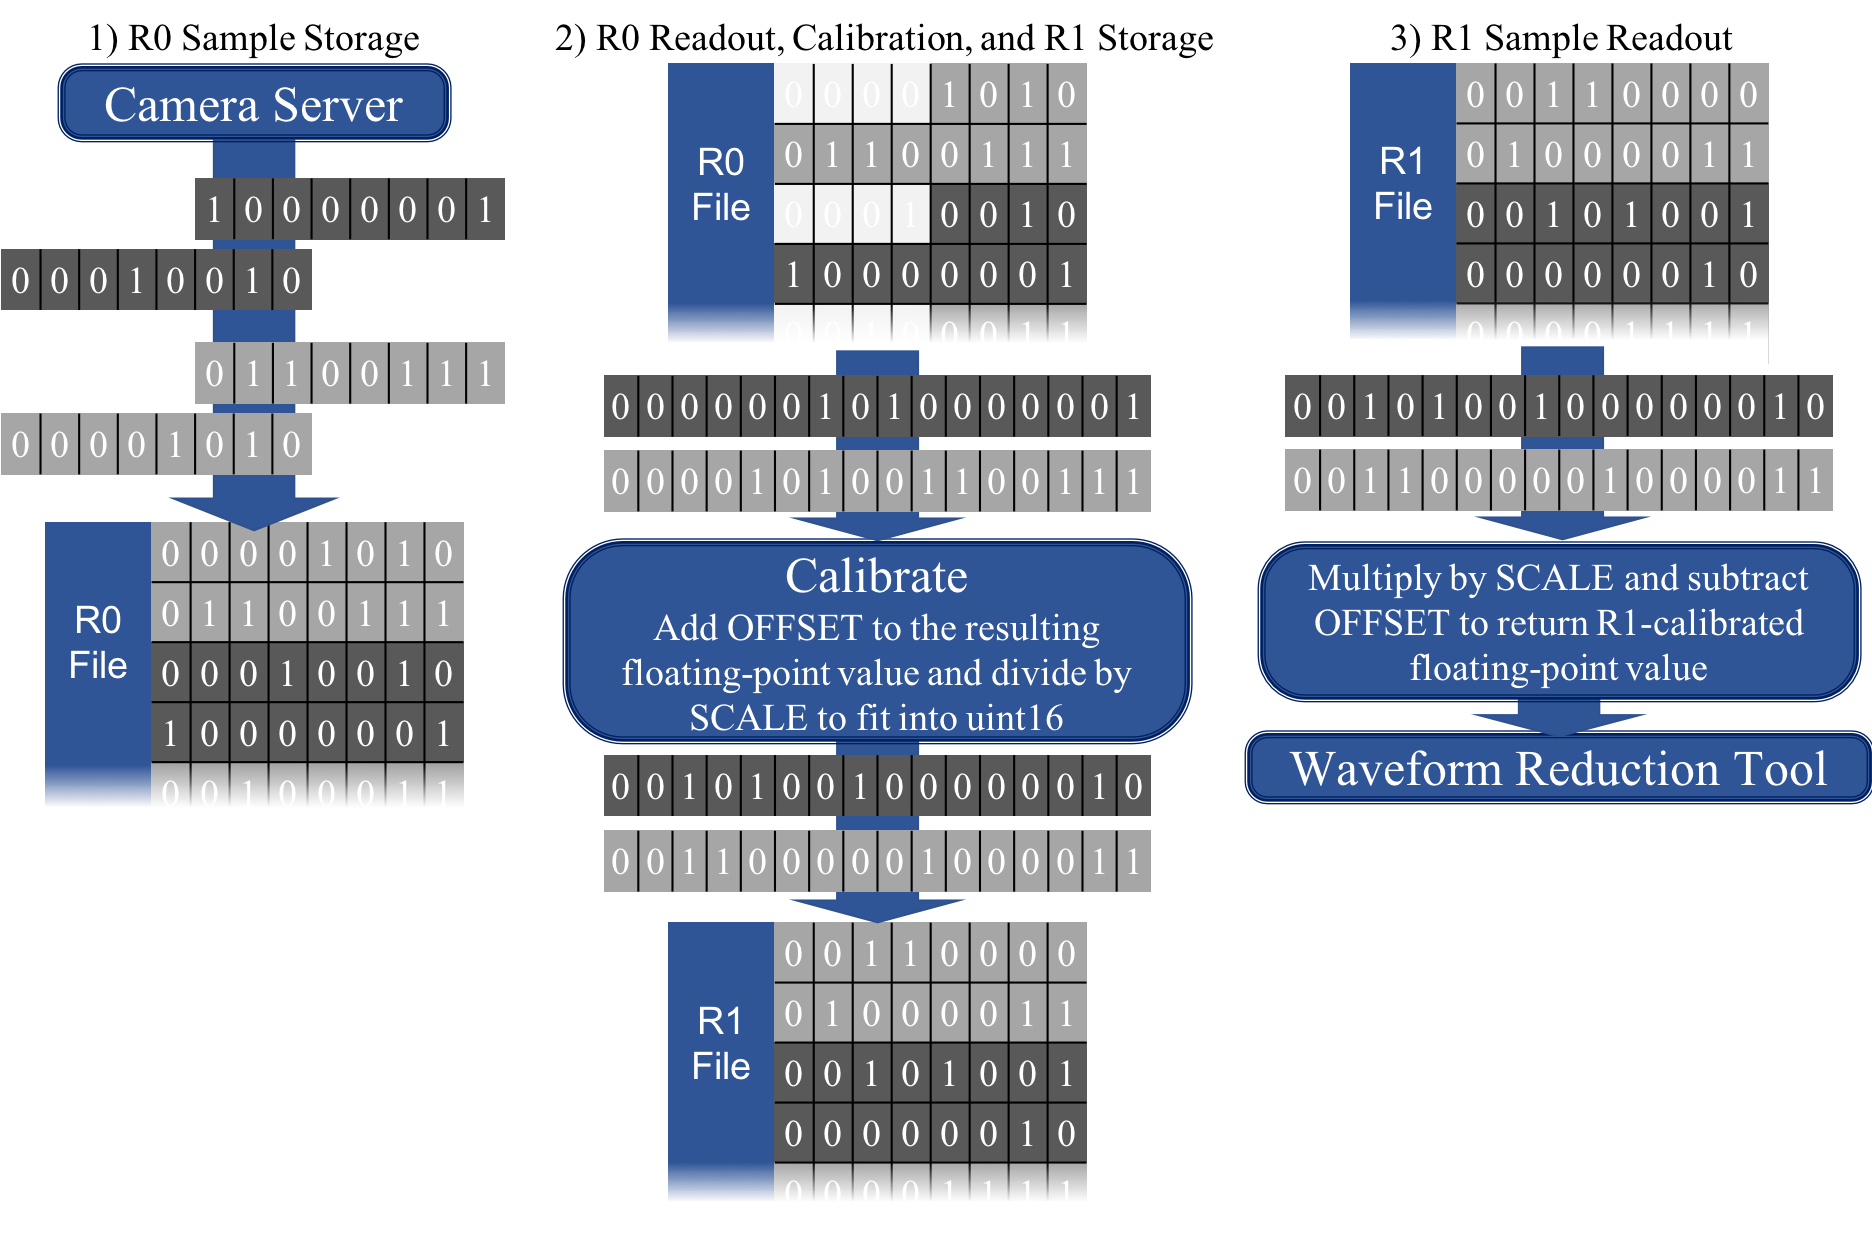
\includegraphics[width=\textwidth]{tio}
  \captionsetup{singlelinecheck=off}
  \caption[Simple overview of the data-flow for waveform samples within the TARGET libraries]{Simple overview of the data-flow for waveform samples within the TARGET libraries:
  \begin{enumerate}[label={\arabic*)}]
  \item 8-bit/char packets are sent from the TARGET FPGA and stored directly to file. A waveform sample is 12-bit, therefore the first four bits of the first 8-bit sample packet are used to indicate sample order.
  \item When reading a sample from the R0 TIO file, the first four bits are ignored, and the remaining twelve bits are combined into an unsigned 16-bit sample. The samples are passed to \pkg{TargetCalib} for calibration. The resulting calibrated floating-point sample is scaled and offset to fit into an unsigned 16-bit integer for storage.
  \item When reading a sample from a R1 TIO file, the entirety of the two 8-bit packets are kept and combined. The value is returned to floating-point format using the OFFSET and SCALE stored in the file header.
  \end{enumerate}
  
  Although only the samples are shown here, all other waveform data is also sent along this stream, including ASIC and Channel number, indicating the start of a new waveform. 
  }
  \label{fig:tio}
\end{figure}

The file format used to store waveforms from \gls{target} modules is a custom \gls{fits} format defined by \pkg{TargetIO}, hereby referred to as the \gls{tio} format. This library is always used to read and write waveform and header (information such as observation time) data to and from the \gls{tio} file. \gls{tio} files can either contain \textit{R0} (uncalibrated)  or \textit{R1} (low-level calibrated) waveform data. Each sample in a waveform is stored to file as an unsigned 16-bit integer. The raw waveform digital counts measured by the camera are serialised in an unsigned 12-bit integer format, and the data packets received from the \gls{target} \gls{fpga} are 8-bit in size, therefore the first 4 bits of a waveform sample inside an \textit{R0} \gls{tio} file are not used. When storing calibrated waveforms, the post-calibration floating-point sample is scaled and offset to fit the full 16-bit unsigned integer. These scale and offset values are stored in the file header and automatically applied to convert the sample back into floating-point format when read. Figure~\ref{fig:tio} demonstrates the data-flow processes involving the \gls{tio} files.

To ensure the full efficiency of the \cpp~library is exploited via the Python wrapper, I contributed the |WaveformArrayReader| class, which, when passed a contiguous block of memory (such as a \lstset{language=Python}|numpy.array|), promptly fills the array with the entire camera's waveform data for that event. For example, to read an \textit{R1} \gls{tio} file from Python:

\begin{lstlisting}[language=Python]
import numpy as np
from target_io import WaveformArrayReader

# Create the reader and get the number of pixels and number of samples from the header
reader = WaveformArrayReader("/path/to/file/Run17473_r1.tio")
n_pixels = reader.fNPixels
n_samples = reader.fNSamples

# Generate the memory to be filled in-place
waveforms = np.zeros((n_pixels, n_samples), dtype=np.float32)
first_cell_ids = np.zeros(n_pixels, dtype=np.uint16)  # Storage cell id for the first sample of the event per pixel

# Fill the arrays
event_index = 20
reader.GetR1Event(event_index, waveforms, first_cell_ids)
# `waveforms' array is now filled with entire event's waveform data
\end{lstlisting}

\subsection{\pkg{TargetCalib}}

To correct for the effects of the \gls{target} electronics on the waveforms, \pkg{TargetCalib} was built. I have led the development of this package since its early development. The calibrations performed by this library are detailed in Chapter~\ref{ch5-calibration}. This package has also been adopted by \gls{sct} recently. The main classes in the library include:

\lstset{language=C++}
\begin{description}
\item [\textbf{PedestalMaker}] Generates the \textit{Pedestal} calibration file.
\item [\textbf{TfMaker}] Generates the \textit{Transfer Function} calibration file.
\item [\textbf{Calibrator}] Applies the aforementioned calibration files to the waveform samples.
\item [\textbf{Mapping}] Handles the files containing the camera's pixel mapping, and provides an interface to the information. This class is necessary due to the non-intuitive mapping between physics pixel position, and order of pixel readout (Figure~\change{figure showing the pixel positions, camera or module?}). Most commonly, this mapping is used for the plotting of camera images. The class is compatible with the mapping of any square-pixel telescope, and customisable to provide the mapping of the pixels in a single module, the mapping of the superpixels, the mapping of the modules, or the neighbours to a pixel/superpixel/module. This class will be deprecated once the central \gls{cta} database of telescope configurations exists.
\item [\textbf{CameraConfiguration}] Provides an interface to certain camera-version dependant variables. Currently the variables that might change with camera-version (stored in the \gls{tio} file header) include number of storage cells, pixel mapping, and reference pulse shape. The correct version of the parameter is returned according to the camera-version provided, allowing for the automated processing of the data of different camera versions. This class will also be replaced by the central \gls{cta} database.
\end{description}

Efforts are being made to improve the \pkg{TargetCalib}'s (more specifically the |Calibrator| class's) efficiency in terms of both memory and processing time, as it will need to meet the \gls{cta} Requirements for \textit{Online Analysis} (Chapter~\ref{ch3-architecture}). It is possible that in the future there will be two separate |Calibrator| classes for the \textit{Online} and \textit{Offline Analyses} respectively.

\section{Reduction Tools}

Tools used to process the waveforms in order to either characterise the camera or progress down the data-level-chain (Figure~\ref{fig:dataflow}) are often referred to as ``reduction tools''. Within the \gls{chec} group we utilise Python for all of our waveform reduction. We made this choice due to its high popularity for data science and signal processing and its extensive library of statistical and numerical packages. The most important examples of these packages include:

\begin{description}
\item [\textbf{NumPy\footnotemark}] \footnotetext{http://www.numpy.org/} Enables the efficient processing of numerical data. This is accomplished using their powerful N-dimensional array object known as a |numpy.array|. At the lowest level, a |numpy.array| is a contiguous block of memory much like a C array. However, NumPy defines many statistical methods which utilise optimised low-level C and Fortran operations to process the contained data in the most efficient way possible, often performing better than handwritten C or Fortran.
\end{description}

Different reduction packages may be designed with different purposes, but each can potentially import methods from another, which is especially simple to do when developing in Python. Although many other \gls{cta} groups have also adopted Python for their waveform reduction software, it is not a standard across \gls{cta}.

\subsection{\pkg{ctapipe}}

Waveform data from each \gls{cta} telescope must be processed and combined using standardised approaches, such that the data at each processing stage is compatible with the next, and the resulting reduced data and shower reconstruction is of good quality. This was the motivation for the design of the \textit{Data Processing Level} architecture (Section~\ref{section:data_levels}). The most reliable way to ensure this architecture is adhered to was to create a single data processing pipeline to transform \textit{DL0} waveforms into \textit{DL3} reduced shower parameters. The primary prototype for this purpose that has been developed among members of the \gls{cta} Consortium is \pkg{ctapipe}.



\subsection{\pkg{CHECLabPy}}

\section{Science Tools}

\subsection{\pkg{GammaPy}}

\subsection{\pkg{CTOOLS}}
%     \chapter{\label{ch5-calibration}Calibration} 

\minitoc

\notes[inline,caption={}]{
	\section{Plan}
	\subsection{Topics}
	\begin{itemize}
		\item Pedestal subtraction
		\item Transfer functions
		\item Gain Matching
		\item SPE
		\item Flat fielding
		\item Time correction
		\item Future
		\begin{itemize}
			\item Live calibration
		\end{itemize}
	\end{itemize}
	\subsection{Questions}
	\begin{itemize}
		\item TARGET architecture diagram, Wilkinson ADC 
		\item How much detail about all the TF approaches do I go into?
	\end{itemize}
}


\change[inline]{Flow diagrams? See Cyril talk 18/07/06 camera calibration call}

\lstset{language=Python}

\section{Introduction}

In order to obtain meaningful and reliable results from the camera, a number of calibrations must be applied to the waveforms read. A primary objective of my DPhil was to investigate the most optimal and efficient approaches for these calibrations (in accordance with the \gls{cta} requirements described in Chapter~\ref{ch3-architecture}), and to determine if additional calibrations are required.

When I joined the \gls{chec} development, the calibration discussion was still in its infancy. Some approaches had been tested in a laboratory environment \cite{Bechtol2012}, but there had been little discussion on how exactly the calibrations could be applied efficiently in an analysis pipeline, where one might not be able to use the same detailed calibration due to limited resources (such as memory and processing time). A major contribution of my DPhil was to prototype the calibration procedures, develop an approach for a calibration pipeline, write the software to perform such a pipeline, and finally assess its performance. This was an iterative process, the development of which is still ongoing. However, a procedure now exists that allows us to obtain meaningful results from the waveform data, a capability that is of paramount importance in the commissioning of the camera.

In this chapter I will outline each of the calibration steps that are presently adopted for \gls{chec}. They are introduced in the general order that they are applied, and split into the categories of \gls{target} \gls{asic}, photosensor, and "other" calibrations.

\section{TARGET Calibration}

The calibrations described in this section relate to the \gls{target} module. As detailed in Chapter~\ref{ch2-mechanics}, the \gls{target} \gls{asic} is responsible for the sampling, digitisation and readout of the waveform data. As a result, there are two calibrations that are solely related to the \gls{target} \gls{asic}: electronic pedestal subtraction and the linearity correction via the transfer function. 

The functional block diagram of the \gls{target} \gls{asic} in Figure~\ref{fig:target5diagram} outlines the electronics that require calibration, and can be used as a reference in the following descriptions.

As the calibrations in this section are very low-level, and related to \gls{chec}'s specific \gls{fee}, they are handled by the TargetCalib library (Chapter~\ref{ch4-software}).

\subsection{Electronic Pedestal Subtraction}

\begin{figure}
\begin{minipage}[t]{.49\textwidth}
  \centering
  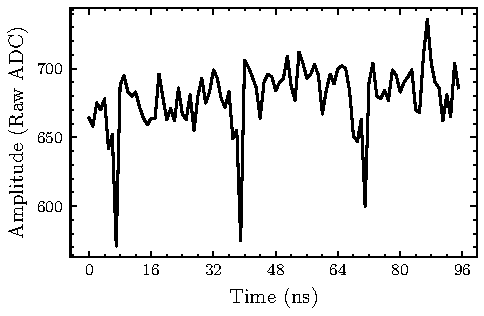
\includegraphics[width=0.92\textwidth]{rawwf_10} 
  \captionof{figure}[Raw waveform]{TARGET-C waveform as read out from CHEC-S, showing the electronic pedestal in the absence of any other input, before any calibration is applied.}
  \label{fig:rawwf}
\end{minipage}%
\hfill
\begin{minipage}[t]{.49\textwidth}
  \centering
  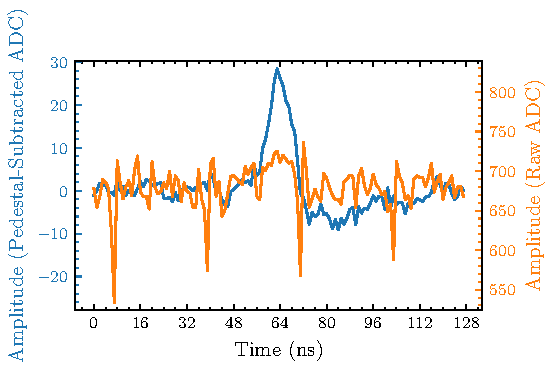
\includegraphics[width=\textwidth]{pulse_raw_vs_pedestal}
  \captionof{figure}[Comparison of pedestal-subtracted waveform with raw waveform]{CHEC-S waveform  containing a \SI{5}{\pe} pulse, before and after pedestal subtraction.}
  \label{fig:pulse_raw_vs_pedestal}
\end{minipage}
\end{figure}

\begin{figure}
  \begin{subfigure}[b]{0.49\textwidth}
    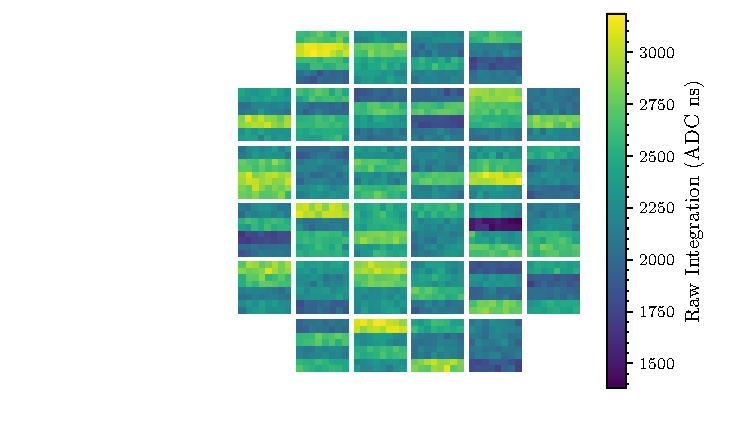
\includegraphics[width=\textwidth]{r0_cherenkov_image_mirrored_cropped}
    \caption{Raw image.}
    \label{fig:r0_cherenkov_image_mirrored_cropped}
  \end{subfigure}
  \hfill
  \begin{subfigure}[b]{0.49\textwidth}
    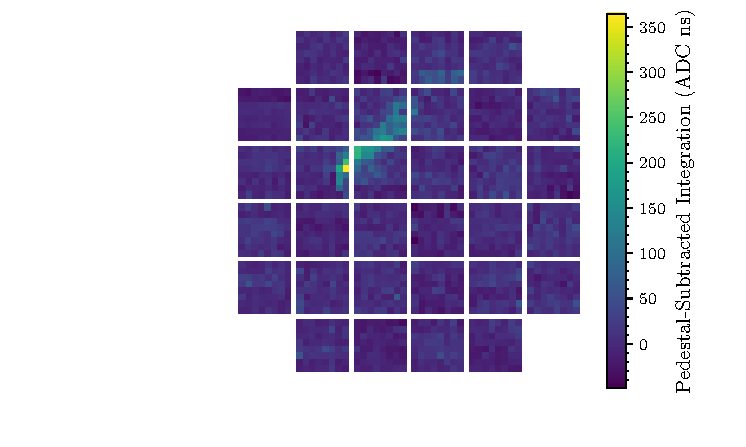
\includegraphics[width=\textwidth]{r1_cherenkov_image_mirrored_cropped}
    \caption{Pedestal-subtracted image.}
    \label{fig:r1_cherenkov_image_mirrored_cropped}
  \end{subfigure}
  \centering
  \begin{subfigure}[b]{0.49\textwidth}
    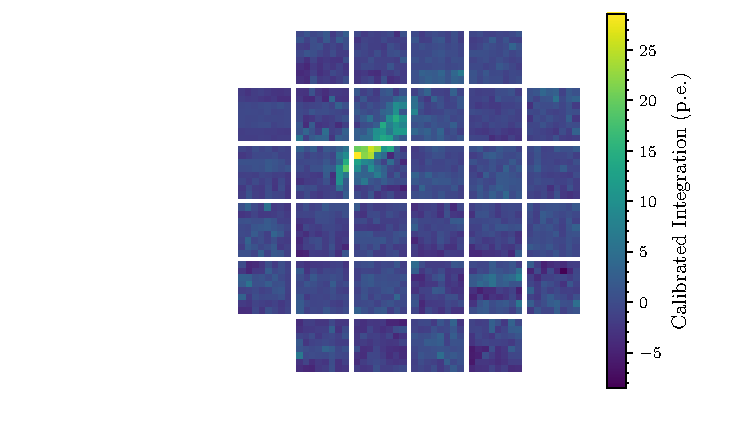
\includegraphics[width=\textwidth]{r1pe_cherenkov_image_mirrored_cropped}
    \caption{Final calibrated image.}
    \label{fig:r1pe_cherenkov_image_mirrored_cropped}
  \end{subfigure}
  \caption[Comparison of calibration stages with a Cherenkov shower image.]{The same image of a Cherenkov shower taken with CHEC-M, but at different stages of calibration. An integration window was chosen using the \textit{Neighbour Peak Finding} technique (Chapter~\ref{ch6-reduction}) on the \si{\pe} calibrated waveforms. The same samples were then integrated for each of the calibration stages.}
\end{figure}

The most important, but also the simplest, calibration to apply ti the waveform data is the subtraction of the electronic pedestal. Each cell in the storage array of the \gls{asic} is a unique capacitor. For a specific \gls{vped}, each capacitor has its own resulting electronic pedestal value. As each sample of the waveform corresponds to a single storage cell, each sample therefore has a unique pedestal value to be subtracted. This is apparent in Figures~\ref{fig:rawwf}~and~\ref{fig:pulse_raw_vs_pedestal} where the variation from sample-to-sample is very large in the raw waveform, and the low-amplitude pulses are almost indistinguishable. The fluctuations in the raw waveforms between pixels is also significant, to the point where low-amplitude Cherenkov showers are undetectable in the camera (Figure~\ref{fig:r0_cherenkov_image_mirrored_cropped}). However, the dominating variations are between \glspl{asic}. As a result, the outlines of the \glspl{asic} are the dominating feature in camera images containing raw samples, such as Figure~\ref{fig:r0_cherenkov_image_mirrored_cropped}. With a pedestal-subtraction calibration alone, the waveforms are transformed into a state in which a moderate amount of Cherenkov shower assessment can be performed, as demonstrated in Figure~\ref{fig:r1_cherenkov_image_mirrored_cropped}.

\begin{figure}
	\centering
    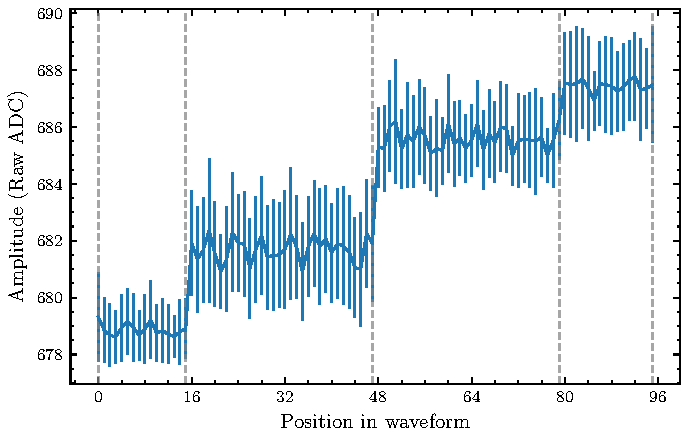
\includegraphics[width=\textwidth]{cellwf_15} 
	\caption[Storage-cell-amplitude dependence on position in the waveform.]{Average amplitude of the electronic pedestal for a single storage cell in a TARGET-C ASIC, at different positions in the waveform. Error bars indicate the standard deviation of the amplitudes. The grey dashed lines indicate the position of the block edges in the waveform for this cell. The average of the values inside each block segment equals the pedestal value stored in the lookup table for that cell, in each of those block positions.} 
	\label{fig:cellwf}
\end{figure}

There are $2^{14} = 16,384$ storage cells per channel (for \gls{chec-m}, $2^{12} = 4096$ for \gls{chec-s}\otherch{Make sure to mention about the difference in number of cells for checs in ch2}), therefore one could naively conclude that there are $32 (Modules) * 64 (Channels) * 16,384 (Cells)$ pedestal values to keep record of. However, an additional characteristic of the \gls{target} \gls{asic} is that the pedestal amplitude depends on the position in the waveform. The source of this characteristic is due to the fact that the storage cell blocks are not entirely decoupled from each other; the discharge of one block affects adjacent blocks. This effect is apparent in Figure~\ref{fig:cellwf}, where the pedestal amplitude of a single cell changes depending on the position of its parent block in the waveform. Consequently, an extra dimension of ``position in waveform'' must be considered in the waveform lookup table.

\subsubsection{Generation}

In order to perform the pedestal subtraction, one must first generate a lookup table of pedestal values. This can be easily obtained with a calibration run where the voltages across the photosensor are disabled, and forcing the camera to trigger (with either an external pulse generator, or internally via software) to obtain a large amount of waveform data. Typically around 30,000 events provide enough samples for every storage cell, in every waveform position, to have at least 10 entries. The samples are then collected as a running average with the dimensions $[Module, Channel, Starting Block, Blockphase+Sample\_i]$, where the $Starting Block$ is the storage block that the first sample in the waveform belongs to, $Blockphase$ is the cell index within the storage block that the waveform begins on, and $Sample\_i$ is the index of each sample in the waveform. This is illustrated in Figure~\change{include figure, and edit to use bp 8 and 12}, where for these two readout windows shown, the pedestal running average |Pedestal[TM][CHANNEL][9][8:103]| and |Pedestal[TM][CHANNEL][8][12:107]| will be contributed to, respectively.

The TargetCalib library handles the pedestal lookup table generation, and stores it into a \gls{fits} file. A new pedestal file is typically generated at the start of each new dataset, as the dependencies on temperature and evolution with time are still being investigated.

\subsubsection{Application}

To apply the pedestal, the entry within the lookup table that corresponds to each sample is subtracted from the waveform. The result of the subtraction can be seen in Figures~\ref{fig:pulse_raw_vs_pedestal}~and~\ref{fig:r1_cherenkov_image_mirrored_cropped}. 

\subsubsection{Performance}

\begin{figure}
	\centering
    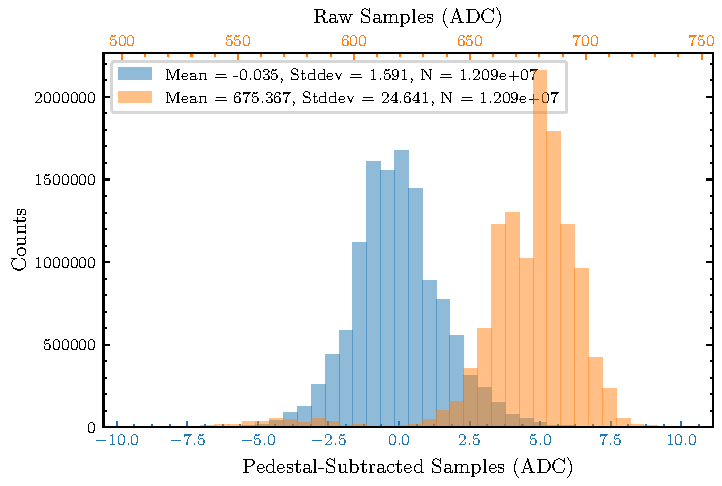
\includegraphics[width=\textwidth]{pedestal_hist} 
	\caption[Spread of electronic-pedestal values before and after the pedestal subtraction.]{Spread of electronic-pedestal values before and after the pedestal subtraction for a single TARGET-C channel. The waveforms used to create the pedestal lookup table are separate to those used in these histograms.} 
	\label{fig:pedestalresiduals}
\end{figure}

The primary quantification of this calibration's performance is the standard deviation of electronic-pedestal samples that have had separately-created pedestal values subtracted from them. Figure~\ref{fig:pedestalresiduals} demonstrates the performance of the pedestal subtraction for a \gls{targetc} channel, achieving a residual variation of \SI{1.6}{ADC} (approximately \SI{0.5}{\pe})\final{update value}.

\subsection{Transfer Function}

The other calibration related to the digitisation and readout inside the \gls{target} \gls{asic} is caused by the non-linearities in the storing and reading of charge to and from the storage cells. The components responsible for the need for this calibration are the sampling array, gain/buffer amps, and the Wilkinson \glspl{adc}, seen in Figure~\ref{fig:target5diagram}. The non-linearity of these components is propagated to the sample readout - a sample with twice the amplitude input into \gls{target} will have less than twice the amplitude when readout.

To correct for this non-linearity, a look-up table is generated to convert from the sample amplitude that is read out from the \gls{asic} (in \si{ADC}) to the sample amplitude that is input into the \gls{asic} (in \si{mV}). This look-up table is known as the Transfer Function. As one might expect, each sampling cell has its own linear response to account for, and therefore a look-up table is typically required at least per channel and per sampling cell, however a noticeably improved performance is observed by considering a Transfer Function per storage cell \otherch{need to show this, maybe in TF Investigations appendix?}.

There are two forms of Transfer Function that have been considered for \gls{chec}, distinguished by the type of input used to generate them. A \gls{dc} Transfer Function is created by applying a constant \gls{dc} input of known voltage into the module, and iterating over the full dynamic range by varying the voltage. An \gls{ac} Transfer Function is generated by inputting a pulse of a known amplitude with a shape expected from the photosensor, and iterating as with the \gls{dc} approach. During previous investigations of the \gls{target} module, where sinusoidal signals were input into the module, a dependence on the signal frequency and input amplitude was observed that acts to further reduce the output amplitude \cite{Bechtol2012}\cite{Albert2017}. The source of this dependence was deemed to be due to the amplifiers, which cannot slew fast enough to keep up with the input signal if the frequency and amplitude are large. Due to the use of a pulse to generate the \gls{ac} Transfer Functions, the result inherently includes the correction required for the frequency that the pulses correspond to. 

\begin{figure}
  \begin{subfigure}[b]{0.49\textwidth}
    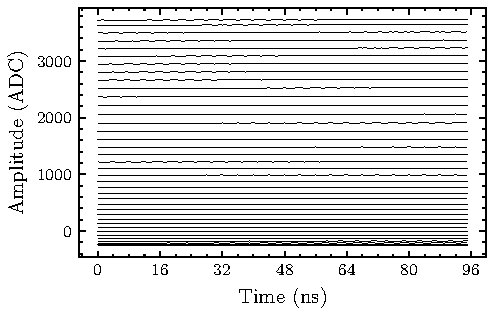
\includegraphics[width=\textwidth]{generation_t5}
    \caption{DC Transfer Function input, measured with TARGET~5.}
    \label{fig:generation_t5}
  \end{subfigure}
  \hfill
  \begin{subfigure}[b]{0.49\textwidth}
    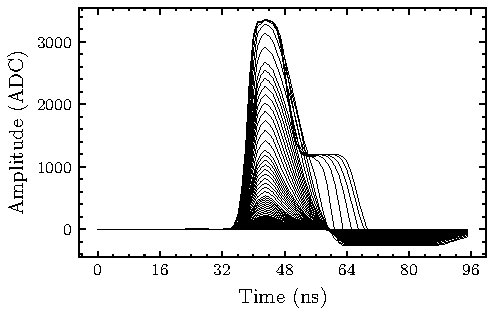
\includegraphics[width=\textwidth]{generation_tc}
    \caption{AC Transfer Function input, measured with TARGET~C.}
    \label{fig:generation_tc}
  \end{subfigure}
  \caption[Transfer Function generation waveforms.]{Multiple average waveforms, increasing in amplitude. Each average contains 1000 waveforms from the same single channel. These waveforms cover the full dynamic range of the TARGET ASIC, and are used as inputs to generate the DC and AC Transfer Functions, respectively. The saturation behaviour of the TARGET C ASIC can be seen in the high amplitude waveforms in (b).}
\end{figure}

\begin{figure}
  \begin{subfigure}[b]{0.49\textwidth}
    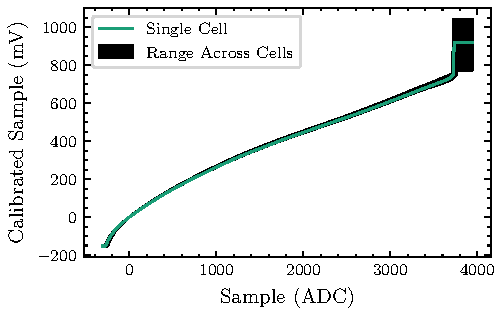
\includegraphics[width=\textwidth]{lookup_t5}
    \caption{DC Transfer Function lookup table, measured with TARGET~5. Contains 64 Transfer Functions, one for each Sampling Cell.}
    \label{fig:lookup_t5}
  \end{subfigure}
  \hfill
  \begin{subfigure}[b]{0.49\textwidth}
    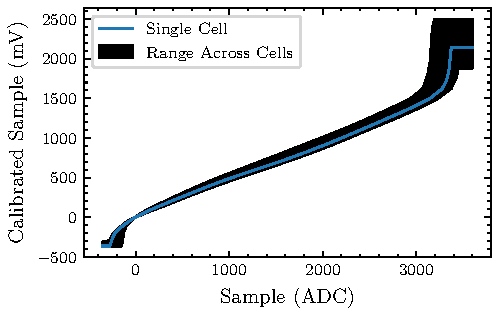
\includegraphics[width=\textwidth]{lookup_tc}
    \caption{AC Transfer Function lookup table, measured with TARGET~C. Contains 4,096 Transfer Functions, one for each Storage Cell.}
    \label{fig:lookup_tc}
  \end{subfigure}
  \caption[Transfer Function lookup tables.]{The Transfer Function lookup tables for a single channel.}
\end{figure}

\subsubsection{Generation (\gls{dc} Transfer Function)}

During the commissioning of \gls{chec-m}, a \gls{dc} Transfer Function was used with no \gls{ac} corrections. To generate this Transfer Function, the internal input pedestal voltage (Vped) setting is used to apply a \gls{dc} voltage offset of known amplitude. By repeating the process for Vped values from \SI{500}{mV} to \SI{1700}{mV}, in steps of \SI{25}{mV}, the full dynamic range of the module is explored, covering the range \SI{-250}{ADC} to \SI{3700}{ADC} (Figure~\ref{generation_t5}). The running averages of the ADC samples are grouped and monitored according to $[Module, Channel, Sampling~Cell, Input~Amplitude]$, utilising every sample in the waveform. Around 1,000 events are required to provide sufficient statistics.

The second step in the generation of the \gls{dc} Transfer Function is to linearly interpolate the running averages at the ADC points defined by the user. This provides a lookup table of \si{mV} values with dimensions $[Module, Channel, Sampling~Cell, ADC~Value]$ that can be used to provide a calibrated value for a measured ADC value. The lookup table for a single channel is illustrated in Figure~\ref{fig:lookup_t5}. This table is saved to a \gls{fits} file, ready for application. A fresh \gls{dc} Transfer Function lookup table was typically created once a day during the \gls{chec-m} commissioning.

\subsubsection{Generation (\gls{ac} Transfer Function)}

\begin{figure}
	\centering
    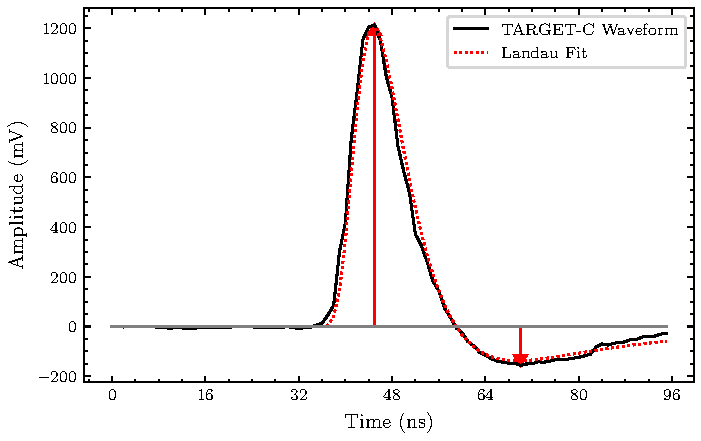
\includegraphics[width=\textwidth]{tf_pulse_fit} 
	\caption[Fit of the waveform in order to extract samples to generate the AC Transfer Function.]{An example of the amplitude extraction used for generating the AC Transfer Function. The waveform is fit with two Landau functions (red curve). The samples of the waveform that occur at the time of the minimum and maximum of the fit (red arrows) are used as the inputs to the AC Transfer Function.} 
	\label{fig:tf_pulse_fit}
\end{figure}

As the ability to internally set a \gls{dc} voltage with a known amplitude via the Vped was removed in \gls{targetc} (see Chapter~\ref{ch2-mechanics}) \otherch{more precise ref, and remember to mention this change}, and the ability to input a \gls{dc} voltage externally is prohibited by the \gls{ac} coupling of the module \otherch{remember to introduce ac coupling}, the decision was made to transition to an \gls{ac} Transfer Function that uses the expected pulse shape as an input. This approach therefore corrects for the \gls{ac} effect with the appropriate frequency. However, in order to externally input pulses from a pulse generator the module must be removed from the camera. Therefore, the \gls{ac} Transfer Function is only generated once in the present calibration pipeline.
	
The full dynamic range is once again probed, by injecting pulses of varying amplitude. In order to extract the values that correspond to negative amplitudes in this method, the amplitude of the input undershoot is also monitored. Only the samples that correspond to the maximum of the input pulse (and minimum of the undershoot) has a ``true'' amplitude of the input amplitude. Therefore, to extract the correct samples, each waveform is fitted with two Landau functions, a fair approximation to the pulse shape (Figure~\ref{fig:tf_pulse_fit}). Consequently, only two samples are extracted per waveform, requiring a much larger population of events (\utilde200,000) in order to generate a reliable running average grouped according to $[Module, Channel, Storage Cell, Input Amplitude]$. It is important to note that a Transfer Function per storage cell was adopted for \gls{targetc}, as it was found to significantly improve the residuals (see Appendix~\ref{a1-tf} for further discussion).

The second step in the generation of the \gls{ac} Transfer Function is identical to that in the \gls{dc} case. The resulting lookup table for a single channel can be seen in Figure~\ref{fig:lookup_tc}.

\subsubsection{Application}

Irrespective of the Transfer Function type, the lookup tables are stored in a format which enables them to be applied identically. When calibrating an ADC sample, the relevant lookup table is obtained according to the channel and cell of the sample, and is linearly interpolated to provide the calibrated \si{mV} value for the specified ADC value.

\subsubsection{Performance}

Due to its complexity and variety of approaches, the Transfer Function is still one of the most actively discussed aspects of the \gls{chec} calibration, and holds the highest potential for improvements among the different calibrations. Some possibilities for improvement include:
\begin{itemize}
	\item An improved sample extraction method for the \gls{ac} Transfer Function Waveform,
	\item The possibility for a \gls{dc} approach for \gls{targetc},
	\item Returning to the approach described in earlier \gls{target} studies where the pedestal is included inside the Transfer Function \cite{Albert2017},
	\item Alternatives to linear interpolation, such as Piecewise Cubic Hermite Interpolating Polynomial (PCHIP),
	\item Exchanging the lookup table for a parametrised regression characterisation of the Transfer Function (such as a high-order polynomial),
	\item Deciding between "per storage cell" or "per sampling cell",
	\item Inclusion of temperature corrections.
\end{itemize}
Appendix~\ref{a1-tf} provides some insight into the current progression in these active investigations.

Assessing the performance of the Transfer Functions is a more complicated task than for the pedestals. We are no longer comparing to a null signal, and instead comparing to an input amplitude which contains its own uncertainty, and could potentially be incorrect. So while the performance results may indicate that the residuals of the Transfer Function are small, this does not necessarily mean the calibration is accurate. Therefore, the most decisive performance indicator should be one that provides an independent measurement on the ``correct'' amplitude. The most obvious scheme fitting this requirement is the charge resolution, described in Chapter~\ref{ch3-architecture}, the results of which are explored in Appendix~\ref{a1-tf}.

\section{Photosensor Calibration} \label{section:photosensor_calib}

The other primary component in the detector chain that requires calibration is the photosensor itself. As photosensors are a much more common instrument used in a variety of experiments, the calibration procedures required are already well known in the academic community. It is therefore mostly a simple case of adapting existing approaches to fit our requirements.

The typical procedure in Cherenkov camera waveform analysis includes extracting the signal charge from the waveform of each pixel. This procedure, and the different methods to achieve it, is described in Chapter~\ref{ch6-reduction}. The value extracted is typically in digitisation counts or units of voltage, multiplied by time if the charge extraction approach is an integral over the waveform. For example, the units of the extracted charge from \gls{chec-s} using the \textit{Cross-Correlation} method (see Section~\ref{section:crosscorrelation}) is \si{mV ns}. Once extracted, this charge must be corrected for the relative efficiency of its pixel compared to the mean of the camera in order to achieve a uniform response (``flat-fielding''), and then converted into a counting unit that is common among the telescopes in the array (such as photons or photoelectrons), thereby simplifying the processing of array data \cite{Aharonian2004}. This procedure is characterised in the equation: 
\begin{equation} \label{eq:photosensor_calibration}
I_i = \frac{{A_Q}_i - {A_0}_i}{\gamma_{Q}} \times {\gamma_{FF}}_i,
\end{equation}
where 
\begin{itemize}
\item ${A_Q}_i$ is the charge extracted in units of \si{mV ns} for pixel $i$, proportional to the number of photoelectrons,
\item ${A_0}_i$ is the baseline in the absence of a signal for pixel $i$. It should be obtained using the same charge extraction approach used for the signal,
\item $\gamma_{Q}$ is the nominal conversion value from \si{mV ns} to photoelectrons/photons for the entire camera,
\item ${\gamma_{FF}}_i$ is the flat-field coefficient for the pixel $i$,
\item and $I_i$ is the resulting calibrated signal in photoelectrons/photons.
\end{itemize}

In the final calibration design of \gls{cta}, ${A_0}_i$ is intended to be supplied by the telescope alongside the waveforms at regular intervals. The regular updating of this value ensures that any changes to the baseline due to \gls{nsb} or temperature variations (which can also increase \gls{dcr}) are accounted for. However, this parameter was set to zero for the content of this thesis, and was not investigated. Instead, a less effective but simpler baseline subtraction was performed by monitoring the running average of the first 16 samples of the past 50 waveforms for each pixel. This running average was subtracted from each waveform before charge extraction. The remainder of this section will describe how to obtain the other calibration values, $\gamma_{Q}$ and ${\gamma_{FF}}_i$, and the other procedures related to the photosensor calibration.

\subsection{Gain Matching}

\begin{figure}
	\centering
    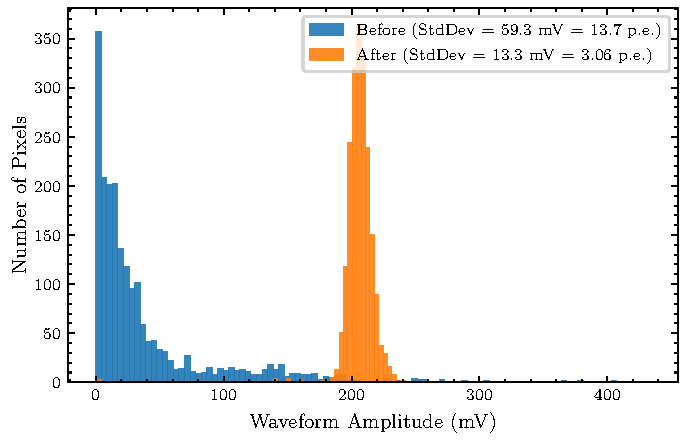
\includegraphics[width=\textwidth]{before_after_gm} 
	\caption[Gain-Matching Residuals]{Comparison between the spread in the average signal amplitude per pixel before and after gain matching, for a dataset with approximately \SI{50}{\pe} average illumination. Every pixel in the camera was included.} 
	\label{fig:before_after_gm}
\end{figure}

The flat-field coefficients, ${\gamma_{FF}}_i$, provide an offline compensation for a variety of photosensor parameters which alter the signal response in the waveform, described in Tables~x\&y\otherch{create table in mechanics chapter that list each parameter for the photosensor, with descriptions and specify if it changes with voltage, temperature, and how it affects signal}. However, as seen in the table, many of these parameters have a dependence on the voltages across the photosensor, which is a controllable value. With the \gls{chec-m} \glspl{mapmt} it is only possible to change the voltage value for an entire module, whereas with the \gls{chec-s} \glspl{sipmt} the voltages can be configured per superpixel (group of four pixels)\otherch{mention superpixels in ch3}. Therefore, voltage values can be selected before data-taking which result in a more uniform signal response across the photosensor. This is referred as ``Gain Matching'', however the name is slightly misleading, as it is the signal that is being matched, not the gain. It is performed by specifying the amplitude (in \si{mV}) that every pixel should be matched to, and then performing the following iterative procedure:
\begin{enumerate}
	\item The camera is uniformly illuminated with approximately \SI{50}{\pe}.
	\item The waveforms are readout, calibrated, and averaged per superpixel/module (excluding any dead pixels).
    \item The peak amplitudes of the average waveforms are extracted.
    \item Each module/superpixel is categorised as being above or below the requested amplitude.
    \item Depending on their category, the voltage setting is increased or reduced by steps of 5 (in units of DAC value), such that it increments closer to the requested amplitude. If the amplitude has been overstepped in the previous measurement, a smaller step value is used. The minimum DAC step value available is 1, which corresponds to $\frac{10}{256}$~V. If the amplitude is not responding to changes in voltage, the pixel is classified as ``dead'', and excluded from the average waveforms.
    \item The new voltage settings are applied and the process is repeated.
\end{enumerate}

In the future, this iterative technique will be replaced with a set of lookup tables for different requested amplitudes. These lookup tables will contain the final voltage settings resulting from this iterative technique. Additionally in the future, the requested signal will not be specified in terms of peak amplitude, but in terms of the \textit{Cross Correlation} charge extraction approach. The improvement in signal response for \gls{chec-s} as a result of the gain matching is shown in Figure~\ref{fig:before_after_gm}, where a response spread reduction of 22\% is achieved.

Tables~x\&y\otherch{update} also show a dependence on temperature for some of the photosensor parameters. The additional benefit of the gain matching is that temperature dependences can also be accounted for, by using the monitored temperature value per module and a lookup table of the appropriate corrections to the voltages, such that a constant signal response is kept across the camera. This particular in-situ calibration has not yet been implemented, but is intended for the future.

\change[inline]{plot with gain vs temperature? maybe some initial results from Yuki}

\subsection{SPE Fitting}

\begin{figure}
	\centering
    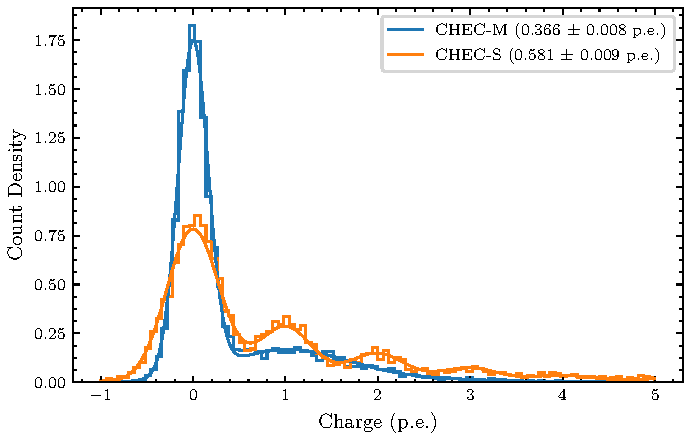
\includegraphics[width=\textwidth]{spe_checm_checs} 
	\caption[Comparison of SPE spectra between CHEC-M and CHEC-S]{Comparison between the spread in the average signal amplitude per pixel before and after gain matching, for a dataset with approximately \SI{50}{\pe} average illumination. Every pixel in the camera was included.} 
	\label{fig:spe_checm_checs}
\end{figure}

Due to the photon-counting nature of \glspl{mapmt} and \glspl{sipmt}, when the signal extracted from a pixel, illuminated with a low light-level (\utilde\SI{1}{\pe}), is accumulated into a histogram, the resulting spectra (Figure~\change{figure of both checm and checs spectra}) show peaks at regular intervals corresponding to the baseline (zeroth peak), \SI{1}{\pe} (first peak), \SI{2}{\pe} (second peak), etc. These spectra are referred to as ``\gls{spe} Spectra''. The physical processes that result in these spectra are well understood for \glspl{mapmt} and \glspl{sipmt}, and therefore analytical formulae \change{check consistency in spelling} exist describing the spectra. When these formulae are fit to the histogram, they can be used to extract certain parameters of the photosensor, including the average incident illumination $\lambda$, in units of photoelectrons. As $\lambda$ provides an absolute illumination value, it allows for the full calibration of expected charge for each filter-wheel position, for each pixel (Section~\ref{section:expected_charge}). This is the first step required in obtaining the flat-field coefficients. For more details on this fitting procedure, and the formulae used to describe the \gls{spe} spectra, refer to Appendix~\ref{a2-spe}.

\subsection{Flat-Field Coefficients}

\begin{figure}
	\centering
    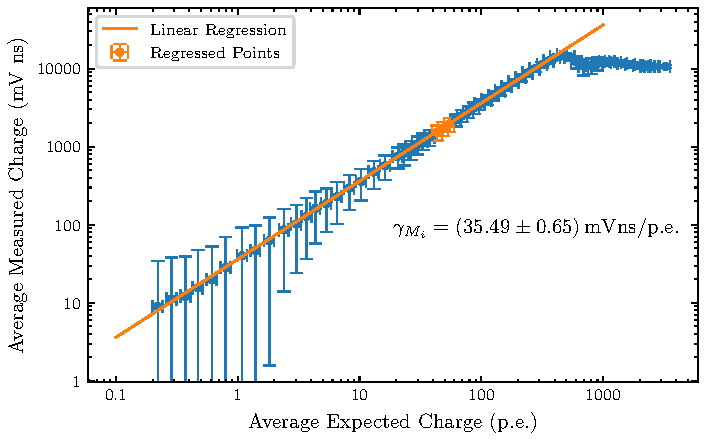
\includegraphics[width=\textwidth]{flat_fielding} 
	\caption[Flat-field calibration]{The average measured charge per illumination for a single pixel. The orange points were used for a linear regression through the origin in order to determine the flat-field coefficients for each pixel.} 
	\label{fig:flat_fielding}
\end{figure}

\begin{figure}
	\centering
    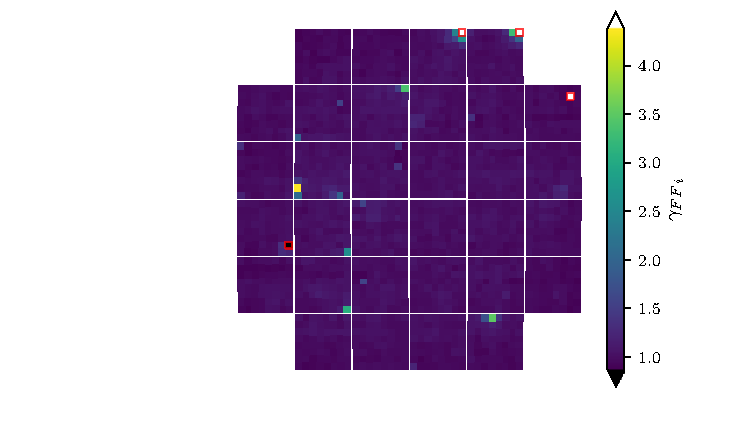
\includegraphics[width=\textwidth]{ff_values_cropped} 
	\caption[Flat-field Coefficients]{Camera image of the flat-field coefficient value, ${\gamma_{FF}}_i$, per pixel. Pixels that were designated ``dead'' or misbehaving are outlined in red, and exist beyond the colour-scale range.}
	\label{fig:ff_values}
\end{figure}

\begin{figure}
	\centering
    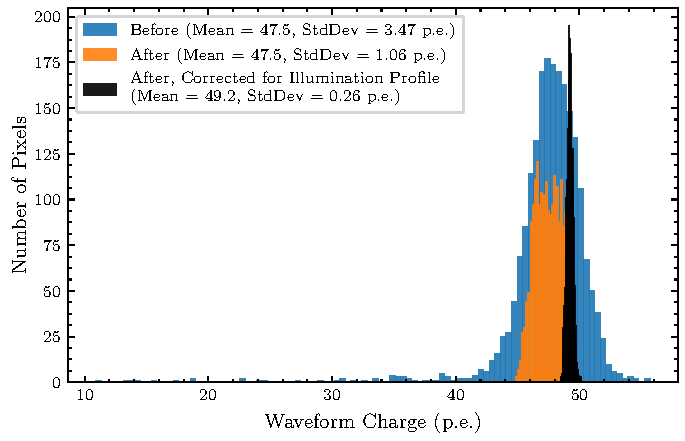
\includegraphics[width=\textwidth]{before_after_ff} 
	\caption[Flat-field Residuals]{Comparison between the spread in the average signal amplitude per pixel before (blue) and after (orange) the flat-fielding calibration. The charges were extracted from a dataset where a theoretical pixel located at the centre of the camera would be expected to have a charge of \SI{47.7}{\pe}. The black histogram contains the charges after the difference in the illumination profile (Section~\ref{section:illumination_profile}) between the pixels was considered, i.e. they contain the charge that would be measured if every pixel was located at the camera centre. Every pixel in the camera was included in the histograms.}
	\label{fig:before_after_ff}
\end{figure}

Once the ``expected charge'' dependence on filter-wheel position/transmission is characterised (Section~\ref{section:expected_charge}), we can calculate the coefficients, ${\gamma_M}_i$, required to convert the average extracted charge (in \si{mV ns}) into the charge we expect (in photoelectrons/photons). The application of these coefficients to the extracted charge has two effects:
\begin{itemize}
\item The signal response between pixels is homogenised - the same average amount of charge will be extracted for any pixel illuminated with an average of N photons.
\item The signal response is converted into the common telescope-array units of photoelectrons or photons.
\end{itemize}
Therefore:
\begin{equation} \label{eq:ff}
{\gamma_M}_i = \frac{\gamma_Q}{{\gamma_{FF}}_i}.
\end{equation}

To obtain ${\gamma_M}_i$ per pixel $i$ in the lab, datasets with around \SI{50}{\pe} expected charge per pixel were produced. For each pixel, the average extracted charge (in \si{mV ns}) was linearly regressed, while forcing the fit through the origin. This regression is shown for a single pixel in Figure~\ref{fig:flat_fielding}. The resulting gradient of the regression is equal to ${\gamma_M}_i$, which was combined with Equations~\ref{eq:photosensor_calibration}~\&~\ref{eq:ff} to obtain the calibrated extracted charge. The value of $\gamma_Q$ obtained for \gls{chec-s} was \SI{32.56}{mVns/\pe}\change{update with latest}, and the spread of $\gamma_{FF}$ across the camera is shown in Figure~\ref{fig:ff_values}. The resulting residual spread in signal response between pixels at an average camera illumination of \SI{47.7}{\pe} is shown in Figure~\ref{fig:before_after_ff}. The final variation in signal response between pixels at this illumination was 0.5\% \change{update when using the lab illumination profile}. The variation in signal responses at other illuminations is shown in Figure~\change{add figure}.

As the flat-field coefficients have been calculated in a manner in which they are unfolded from the illumination profile (by calculating the expected charge individually for each pixel), they are applicable to any environment the camera is used in. Any deviations that are observed in the signal between pixels are then due to the illumination profile present in the environment, and not due to the characteristics of the photosensor. Once the camera is on the telescope, the flat-field coefficients are intended to be routinely updated using the reflection of the LED flashers (Section~\ref{section:peripherals}) in the secondary mirror. This calibration will require an updated illumination profile in order to be performed.

\subsection{Dead Pixels}

Figure~\ref{fig:ff_values} shows that some of the photosensor pixels contained either no signal or an odd signal, resulting in an extreme flat-field coefficient. This was likely due to damage to the pixel during handling, or due to water ingress. However, the four pixels constitute to \SI{0.2}{\percent} of the camera, therefore the camera is still well within the \requirementref{B-TEL-1295 Pixel Availability} \gls{cta} requirement (Chapter~\ref{ch3-architecture}). These pixels were excluded from any calculations involving multiple pixels, including the expected-charge calibration and the camera charge-resolution. 

\section{Saturation Recovery}

\begin{figure}
	\centering
    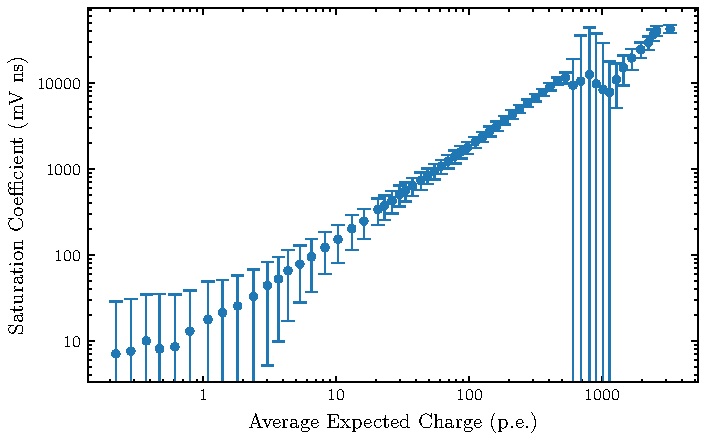
\includegraphics[width=\textwidth]{saturation_recovery} 
	\caption[Saturation Recovery.]{Initial investigation into recovering charge from a saturated waveform for the same pixel as shown in Figure~\ref{fig:flat_fielding}. The saturation coefficient is the integral from just before the pulse maximum, to the end of the waveform readout.}
	\label{fig:saturation_recovery}
\end{figure}

As evident in Figure~\ref{fig:flat_fielding}, high illumination (greater than \utilde\SI{200}{\pe}) measurements are affected by saturation of the detector. The saturation shown is due to the \gls{target} \gls{asic}, which saturates before the photosensor. However, while the height of the pulse increased no further, the excess charge caused the pulse to extend further (Figure~\ref{fig:generation_tc}). Therefore, it could be possible to perform a simple correction for the saturation recovery by utilising this waveform behaviour. A simple, initial investigation into saturation recovery is shown in Figure~\ref{fig:saturation_recovery}, where the waveform was integrated in a window that started just before the pulse maximum, and extended to the end of the waveform. This resulted in an extracted charge that continued to increase with illumination, apart from in the region immediately after saturation. More investigation is required for this calibration.

\section{Timing Corrections} \label{section:timing_corrections}

Due to the routing of the electronics in the front-end, the electrical signal path is slightly different per channel, causing a small difference in apparent arrival of the pulse in the waveform. The relative arrival time per pixel can be seen in Figure~\change{add camera image showing relative time}. 

Not only does this need to be taken into consideration when investigating the timing performance, it also can have a significant impact on the charge extraction performance. This is because the charge extraction approaches typically rely on other pixels (neighbouring or entire camera, see Chapter~\ref{ch6-reduction}) sharing a compatible pulse time. A charge extraction routine that incorrectly extracts the charge by \SI{1}{ns} can have the impact on the charge resolution shown in Figure~\change{show impact of an incorrect time extraction on charge resolution, maybe of just TM?}. Discussions are ongoing on how to best include the timing corrections in the charge extraction.

\section{Future}

During the long development of \gls{chec}, the calibration procedure has evolved significantly. Multiple iterations of the procedures have occurred to:
\begin{itemize}
	\item Accommodate the changes required in the upgrades of hardware (such as from \gls{target5} to \gls{targetc}).
	\item Simplify the calibration to save on computing resources.
	\item Account for additional factors, thereby improving the calibration (such as the \gls{ac} contribution to the Transfer Functions).
\end{itemize}
Therefore, while each iteration improves in one aspect, it may be at the expense of the others. As a result, the \gls{target} calibration procedure described in this chapter appears quite complicated compared to the approaches detailed by \textcite{Albert2017} and \textcite{Bechtol2012}. The next step in the calibration development for \gls{chec} is therefore to review the procedure used, with the aim of producing an approach that is simpler, includes aspects such as temperature dependence, and meets the requirements and processing rates required by \gls{cta}.

%    \chapter{\label{ch6-reduction}Waveform Reduction} 

\minitoc

\notes[inline,caption={}]{
	\section{Plan}
	\subsection{Topics}
	\begin{itemize}
		\item Charge Extraction Methods
		\item Image cleaning
		\item Shower reconstruction
		\begin{itemize}
			\item Hillas
			\item Impact
			\item model
			\item Neural Nets
			\item ++
		\end{itemize}
		\item Energy Reconstruction
		\item Direction Reconstruction
	\end{itemize}
	\subsection{Questions}
	\begin{itemize}
		\item ?
	\end{itemize}
}

\section{Introduction}

Methods for retrieving information about the Cherenkov shower have been a primary component of the Imaging Atmospheric Cherenkov Technique since its inception. Early techniques such as those used in the first observation of TeV Gamma rays from the Crab nebula \cite{Weekes1989} are still utilised in modern \glspl{iact}. These techniques are also applicable to \gls{cta} telescopes, and as \gls{cta} is a large consortium which consists of the worldwide \gls{iact} community, the developers of the reduction approaches for previous \glspl{iact} have brought them forward to \gls{cta}. However, due to:
\begin{enumerate}[label=(\alph*)]
	\item \gls{cta} is to consist of the most advanced \glspl{iact} to date, with higher shower imaging resolution and telescope multiplicity than has previously been available,
	\item the capabilities of digital signal processing has significantly increased in the past decade,
\end{enumerate}
the opportunity for more advanced and more successful algorithms exists for \gls{cta}. Some effort has already been made in this direction, but it is an aspect that is expected to constantly evolve and improve during the lifetime of \gls{cta}. In this chapter I will provide an overview of the existing and in-development reduction techniques utilised to extract the Cherenkov shower signal from the waveforms, and my involvement in designing a charge-extraction technique for \gls{chec-s}. With regards to the \gls{cta} data levels (Figure~\ref{fig:dataflow}), this chapter is mostly concerned with the step from \textit{DL0} to \textit{DL1}.

\section{Charge Extraction Methods}

The immediate step after the waveform calibration is the extraction of signal from the waveforms provided by each camera individually. As a result of the low-level calibration detailed in \ref{ch5-calibration}, the waveforms from each \gls{cta} camera exist in a common state, with no remaining dependencies on the electronics they were produced with. Therefore, the extraction techniques are typically applicable to all \gls{cta} cameras. 

The extraction of signal from a waveform is a very generic problem, allowing for the utilisation of common signal processing techniques that are not unique to Cherenkov shower analysis. The goal is to extract as much signal from the pulse created by the Cherenkov shower light, while simultaneously limiting the inclusion of noise factors\change{reference where noise talked about, talk about all the contributing factors (noise etc.) to waveforms in ch2}. Two quantities are extracted in this stage: the signal charge in each pixel, and the signal arrival time per pixel. 

The total signal charge in a pixel, i.e. the total number of photo-electrons released from the \gls{pmt}'s photocathode, is proportional to the total area below the pulse corresponding to the Cherenkov photons. If the waveforms were completely free of noise, and the readout window was large enough to capture the full Cherenkov signal, a simple integration of the entire readout would be a satisfactory approach for obtaining the signal charge. However, as we do not have the luxury of perfect waveforms, more complex methods are designed. Charge extraction algorithms typically consist of two aspects: how the signal pulse is found, and how the pulse is integrated.

\subsection{Peak Finding} \label{peakfinding}

Two factors must be considered when finding the signal pulse of a Cherenkov shower. Firstly, the majority of camera pixels will not contain any Cherenkov signal while still containing noise. A peak finding technique that assumes a signal exists in the readout will be biased, as it will mistake the noise for signal. Secondly, due to the nature of Cherenkov showers (Chapter~ \change{reference where the time gradient of Cherenkov showers are described}), those pixels with Cherenkov signal will have different arrival times due to the time evolution of the Cherenkov image \change{figure of peak time?}. This time gradient across the image is especially apparent for bright showers at a large core distance from the telescope. The most successful peak-finding technique is one that best accounts for those two factors. Some simple techniques used to define a peak time from a waveform include:
\begin{itemize}
	\item \textbf{Local Peak Finding}: Each waveform is treated independently from the other. The maximum point in the waveform is treated as the peak/arrival time. This approach is intrinsically biased to assume every waveform contains a signal; therefore, in the absence of a Cherenkov signal, the largest noise pulse will be extracted, resulting in a higher total charge than should be obtained.
	\item \textbf{Global Peak Finding}: The waveform from every pixel is combined into an average, from which the maximum point is treated as the peak time for every pixel. This technique is only useful if a large portion of the camera is simultaneously illuminated, such as by a laser in the case of lab commissioning and calibration runs.
	\item \textbf{Neighbour Peak Finding}: The waveforms from the neighbouring pixels are combined into an average, from which the maximum point is treated as the peak time for the pixel-of-interest. This technique is often preferred for Cherenkov images as it has a reduced charge bias (especially if the pixel-of-interest's waveform is not included in the average); pixels with Cherenkov signal typically have neighbours that also contain Cherenkov signal at a correlated time, while the neighbours of empty pixels only contain noise, and therefore a peak time that is uncorrelated to the noise is chosen.
	\item \textbf{Fixed Peak Value}: Due to a reliable definition of the camera trigger and subsequent electronic chain, the position of the pulse in the waveform could consistently be known a-priori, allowing for a fixed peak time. However, this method requires a larger integration window size in order to capture the full pulse in the tail of the Cherenkov shower, which occur at a later time than the initial photons which trigger the camera, therefore resulting in a larger noise included in the signal. However, this technique usually contains the least bias, as no signal is assumed to exist.
\end{itemize}

 A more complex peak-finding technique is the \textit{Gradient Peak Finding} approach. This approach was designed for the VERITAS telescope \cite{Holder2005}\cite{Cogan2006}\cite{Cogan2007}, but is applicable to any \gls{iact} telescope that allows the dynamic specification of an integration window. \textit{Gradient Peak Finding} utilises the gradient profile of the photon arrival time for gamma-induced Cherenkov showers, described in Section~\ref{section:photon_arrival_time} and illustrated in Figure~\change{chec-m pulse time figure}. This peak-finding technique is a two-pass approach performed by first extracting the signal using one of the other methods. The timing information contained within the pixels that survive cleaning (Section~\ref{section:image_cleaning}) can then be used to obtain a relation between ``distance along primary image axis'', $D_{ax}$, and the pulse time, $T_0$. Figure~\change{figure with geometry} illustrates the geometry of $D_{ax}$ with respect to the pixel position. Using the obtained relation between $D_{ax}$ and $T_0$, an example of which is shown in Figure~\change{figure of Dax versus T0 for checm figure}, an unbiased pulse time is obtained for each pixel depending on its position along the image axis.

These peak-finding methods have been described in relation to the maximum of the signal pulse, however they may instead use other characteristic positions of the pulse, such as the half-maximum time on the rising edge, or the centre of gravity of the pulse. Additionally, more advanced peak-finding techniques may up-sample (possibly by zero-padding in the frequency domain via a Fourier transform) or interpolate the signal to obtain a more precise peak time \cite{Cogan2006, Cogan2007}, or even apply low-pass filters in order to remove low frequency baseline noise. The peak finding should be done in conjunction with any timing corrections (\ref{section:timing_corrections}) that may be required.

\subsection{Integration}

Once the peak time has been obtained, the simplest approach to extract the signal is to define an integration window centred about this time. The size of the window needs to be large enough to capture sufficient signal from the pulse, but small enough that not too much noise (\gls{nsb}, dark counts, afterpulsing) is included within the window, thereby maximising the signal-to-noise. Additionally, the camera's pulse shape may not be symmetric, so a better signal-to-noise may be achieved by shifting the window a few samples with respect to the peak time. The optimal integration window size and shift for the \gls{chec-s} waveforms is found to be \SI{5}{samples} and \SI{2}{samples} (i.e. \SI{5}{ns} and \SI{2}{ns}), respectively, according to the investigations performed in \ref{a3-extractors}.

Beyond the simple ``boxcar'' integrator method (where every sample integrated has a weight of 1), other more advanced strategies may define their own alternative approach to extract the charge. One example is the fitting of the signal pulse, with an analytical description of the expected pulse, or with a more unconstrained description such as a cubic spline. A second complex approach is the use of digital filters, which can be used in combination with knowledge of the pulse shape to robustly extract the signal even in the presence of high noise. Such a technique has been designed and adopted for \gls{gct}, referred to as the \textit{Cross-Correlation} method. Due to its adoption and sophistication, it is described here in more detail. 

\subsubsection{Cross Correlation} \label{section:crosscorrelation}

Cross-correlation is a common signal processing technique used as a measure of the similarity between two signals as a function of the displacement in time applied to one of the signals. Given a continuous function $f(t)$ defined between $0 \le t \le T$ and a second continuous function $g(t)$, the cross-correlation between the two functions ($f \star g$) is defined as 
\begin{equation} \label{eq:cc1}
(f \star g)(\tau) = \int_0^T \overline{f}(t)g(t + \tau)dt,
\end{equation}
where $\overline{f}(t)$ is the complex conjugate of $f(t)$ and $\tau$ is the time displacement (also referred to as the ``lag'') between the two functions \cite{wolfram-crosscorrelate}. In descriptive terms, by varying $\tau$, $g(t + \tau)$ will slide past $f(t)$. The cross-correlation for a value of $\tau_1$ is then the integral across $t$ of the product between $f(t)$ and $g(t + \tau_1)$. For a discreet function that is real-valued, such as a sampled waveform, Equation~\ref{eq:cc1} can instead be defined as
\begin{equation} \label{eq:cc2}
(f \star g)\lbrack n \rbrack = \sum_{m=0}^N f\lbrack m \rbrack g\lbrack m + n\rbrack,
\end{equation}
where $N$ is the total number of samples in the waveform and $m$ is the sample displacement. 

An illustration of the \textit{cross-correlation} approach being applied on a \gls{chec-s} waveform is shown in Figure~\change{figure showing the cross-correlation at a few different times, and the different stages, 3 axes, maybe for a low illumination? mention I implemented \ref{eq:cc2} in Python}. Through utilising a template of the expected pulse shape in the absence of noise (hereafter referred to as the ``reference pulse'') features inside the waveform that are correlated with the reference pulse shape are emphasized, while features that do not, such as the electronic noise, are suppressed. Therefore, the peaks in the cross-correlation result correspond to the displacements where the signals match best, and the values of the peaks correspond to an weighted integral of the entire waveform, and can be used as an extracted charge value.

The reference pulse we use for the cross-correlation was obtained via probing the input analogue signal on the \gls{target} module and averaged on an oscilloscope. It was then normalised such that cross-correlation between it, and the reference pulse normalised to have an integral of 1, has a maximum value of 1. This normalisation ensures that the cross-correlation result is in units of \si{mV ns}, and allows an easy conversion into \si{mV} for ``peak-height'' investigations.  An optimised implementation of cross-correlation exists in |scipy.ndimage.correlate1d| \cite{scipy-crosscorrelate}, where the waveforms for every pixel are processed in parallel.

\change{mention negatives of the cc approach, like the emphasis of nsb and cc, here or in appendix?}

\subsection{Approaches Adopted by Other IACTs}

Some examples of approaches adopted by other telescopes are outlined below, to provide an overview of techniques considered by other \glspl{iact}.

\subsubsection{MAGIC}

Members of the MAGIC telescope, \textcite{Albert2008}, performed a study comparing the techniques proposed for their signal reconstruction. Four approaches were compared: \textit{fixed-window}, \textit{sliding-window} with amplitude-weighted time, \textit{cubic spline fit} with integral or amplitude extraction, and \textit{digital filter}. It was concluded that the digital filter, which relies on knowledge of the signal shape to minimise the noise contributions, provided a charge reconstruction with acceptable bias and minimal variance, while remaining stable in the occurrence of small variations in pulse shape and position.

\subsubsection{VERITAS}

Similar to the aforementioned study for the MAGIC telescope, a comparison of charge extraction approaches was performed for VERITAS \cite{Holder2005, Cogan2006, Cogan2007}. Specifically, the extraction methods compared included a \textit{simple-window} using a-priori knowledge of the Cherenkov pulse time in the trace, a \textit{dynamic-window} which slides across the trace to find the Cherenkov pulse, a \textit{trace-fit} evaluator with fits the trace with two exponential functions which respectively describe the rise and fall time of the pulse, a \textit{matched-filter} which ``uses a digital filter based on the assumed shape of the FADC pulse to integrate the charge'' \cite{Cogan2007}, and finally an implementation of the \textit{Gradient Peak Finding} approach described earlier in the chapter. At first glance, some of these approaches bear resemblance to those used by MAGIC, however there are slight differences: 
\begin{itemize}
	\item in the VERITAS pulse fitting technique, an attempt to describe the pulse analytically was made whereas the MAGIC approach used a more loosely defined spline
	\item the filter used by VERITAS is a cross-correlation in Fourier space, whereas the filter used by MAGIC is generated using their knowledge of the noise auto-correlation matrix
\end{itemize}

Either as a result of these differences, or due to the difference in the instruments themselves, the VERITAS \textit{matched-filter} appears to result in a worse reconstruction than one would expect from the conclusion reached by MAGIC. One might justify that this degradation of signal extraction with the \textit{matched-filter} for higher amplitudes is due to a change in pulse shape at higher amplitudes, thereby requiring a different "assumed FADC pulse shape", but it is not clear if that is what is occurring here\change{Garret: However, a thorough investigation of this particular reconstruction is beyond the scope of this work}. These studies conclude that the \textit{matched-filter} ''holds promise`` for reconstructing low charges, whereas while the \textit{trace-fit} performs extremely poor for the low charges (as expected), it performs the best for amplitudes > 4 photoelectrons \cite{Cogan2007}.

\subsubsection{H.E.S.S.}

The standard mode of charge extraction for the \gls{hess} telescopes is to integrate $N$ samples with respect to a fixed, but regularly verified, signal time \cite{Aharonian2004}. \gls{hess} camera electronics underwent an upgrade in 2015/2016, subsequently allowing for the update of the standard extraction mode to also output time-of-maximum and time-over-threshold, and also allowed for full sample readout enabling the utilisation of more complex charge extraction techniques \cite{Klepser2017}\cite{Chalme-Calvet2015}.

\subsubsection{ASTRI}

Contrary to the other techniques described in this section, \gls{astri} took the alternative direction of a hardware-implemented charge extraction, utilising their \gls{citiroc} \gls{asic}. The pulse from their \gls{sipmt} is amplified and shaped (with both a high-gain and low-gain channel) with a constant shaping time of \SI{37.5}{ns}. The maximum of the shaped peak-height is then converted into an integrated charge, achieving no more than \SI{1}{\percent} introduced systematic error \cite{Impiombato2017}. The \textit{DL0} and \textit{DL1} formats are therefore identical in \gls{astri}'s case as the charge-extracted value is provided in place of waveforms. However, while this charge-extraction technique is optimised for the \gls{astri} electronics, it removes the flexibility of being able to dynamically select a charge-extraction technique within the software, and adopting new software-based techniques that may be designed in the future.

\subsection{Performance Assessment}

Deciding on which charge extraction method to use is not trivial - as shown in the above discussion, different cameras may perform better with different algorithms. This is anticipated in \pkg{ctapipe} (\ref{ch4-software}), where different |ChargeExtractors| can easily be selected at runtime depending on the camera source.

The assessment technique typically used for charge extractors in the context of \gls{cta} is the Charge Resolution (Section~\ref{section:cr}). A performance assessment of charge extraction techniques for \gls{chec-s} can be found in Appendix~\ref{a3-extractors}.

\section{Next Steps}

The resulting images of the extracted signal per triggered telescope is only the first stage of many to retrieve the properties of the Cherenkov-shower progenitor particle: direction, energy, and class. The direction is necessary to retrieve in order to obtain the source's position and spatial morphology. The energy is desired for studies of the source's spectrum. The class of the progenitor particle (gamma-ray, electron, or cosmic-ray hadron) is required in order to identify the gamma-rays among the cosmic-ray background. All the information required to obtain these progenitor particle properties is contained within the image of extracted charge.

Pixels containing signal from the Cherenkov shower are identified an image cleaning method such as the tailcuts approach: any pixels above a certain signal threshold are kept, and any neighbouring pixels that are above a lower signal threshold are also kept. The thresholds are optimised per telescope using Monte Carlo simulations. The resulting pixels are then parametrised in terms of their second moments. This parametrisation is a predominant \gls{iact} analysis technique that has been utilised in the majority of \gls{iact} experiments. It was first formalised by \textcite{} and has subsequently been known as the Hillas parametrisation. This technique utilises the elliptical shape of the gamma-induced shower images, and provides values for the centre of gravity of the ellipse, its primary axis position and orientation, its width, and its length (Figure~\change{hillas parameterisation figure}.

Using a two-pass selection cut on the images

As shown in Figure~\ref{}



\begin{itemize}
\item The primary axis of the ellipse in the Cherenkov shower image represents the major axis of the Cherenkov shower. Therefore, the location of the source can be found along the primary axis of the ellipse. 
\item The total amount of signal detected from the Cherenkov shower (image \textit{size}) is a direct measure of the total energy released as Cherenkov light, and therefore is a direct measure of the progenitor particle's energy (Section~\change{section in introduction where it is shown that the majority of energy of the gamma-ray is release as cherenkov light}. However, the intensity of light received from the showers is inversely proportional to the distance squared. With knowledge of the distance to the shower core combined with 

Therefore, the combination of shower impact distance and image \textit{size} provide an estimation of the particle's energy.
\item 
\end{itemize}



direction is obtained from the primary axis of the 

As explained in Section 2.1.3, the major axis of the ellipse represents the
shower axis of the extended air shower. In particular, one side of the major
axis points towards the location of the source.

The extraction of this information is much more reliable through the use of the stereoscopic combination of the images from telescopes which detected the Cherenkov shower. However, while the problem of degeneracy in obtaining the location of the source with a single telescope is a difficult problem to overcome, it is not an impossible one.


Reconstruction of showers with a single telescope is more difficult; 

The ability to reconstruct showers with single telescopes is hampered by
the inherent degeneracy in determining which side of the camera field of view (FOV) the shower originated in. In a single telescope analysis, the source location is assumed to lie along the primary image axis, and the distance to it from the image centroid can be calculated according to Lessard et al. (2001). Use

As the focus of this thesis is on the low-level performance of the \gls{gct} cameras, an extended overview of the next stages involved shower reconstruction is not included. However, a brief description of the simple approaches used in the immediate next steps are supplied as context for the results described in \ref{ch8-pipeline}. For a full overview of the next stages in Cherenkov shower reduction, refer to the following publications \change{add publications, perhaps in list?}.

With knowledge of the the 

The purpose of the reduction of \gls{iact} waveforms is to recovery 

Resulting from the extraction of signal from the waveforms, an image of the Cherenkov shower for each of the triggered telescopes is obtained. The purpose of these images is to 


The sum of the charge in each pixel containing a part of the shower is a measure of the total energy released as Cherenkov radiation, which, as explained in Chapter~\ref{ch1-intro}, is a measure of the energy of the shower progenitor particle (cosmic or gamma-ray) \change{make sure to talk about this in introduction. maybe use a more direct reference than just the chapter}. The primary image axis is a measure of the direction of the Cherenkov shower


\section{Image Cleaning} \label{section:image_cleaning}

Once a charge per pixel is obtained, the next stage in reduction is to select the pixels which contain signal from the Cherenkov shower, in order to ease the parametrisation. 

\subsection{Tailcut Cleaning}

\subsection{Wavelets}

\section{Shower Parameterisation}

\subsection{Hillas}

\subsection{Model and Model++}

\subsection{ImPACT}

\subsection{Neural Nets}

\section{$\gamma$-Hadron Separation}

\section{Energy Reconstruction}

\section{Direction Reconstruction}



\change[inline]{advanced techniques that don't fit into these categories, machine learning, photon counting}

%    \chapter{\label{ch7-performance}Camera Performance} 

\minitoc

\section{Introduction}

As discussed in Chapter~\ref{ch3-architecture}, it is important that the \gls{chec} camera meets certain criteria in order for it to be accepted as an in-kind contribution to \gls{cta}. One important subset of the criteria is the camera's performance. The requirements that must be fulfilled are driven by the science goals of \gls{cta}. If a camera does not meet the requirements laid out by the \gls{cta} observatory, then it will be refused as a contribution in its current state, lest the science goals of \gls{cta} are not achieved.

This chapter will cover many of the primary standards used to assess a \gls{cta} camera's performance. The results shown in this chapter are all my own, and are obtained using the procedures defined in the preceding chapters. Two important aspects of the camera's performance which are not included in this chapter are the trigger efficiency and absolute photon detection efficiency. The investigations into these parameters are ongoing, and I have not had direct involvement with these as part of my DPhil.

\section{CHEC-S Monte Carlo Model}

An important preface to reporting on the performance of \gls{chec} is the description of the efforts in generating an accurate model of the camera for use inside the Monte Carlo simulations performed by \pkg{sim\_telarray} (Chapter~\ref{ch4-software}). These simulations allow us to explore the parameter space related to our camera performance more widely, and identify potential issues that cause the real camera to drift away from ideal operation. It is also a necessary step in investigating the on-sky performance of the telescope, as:

\begin{itemize}
\item One does not have prior knowledge of the properties of the light incident on the pixels in the real world.
\item The camera is still being tested in the lab. An on-sky campaign for \gls{chec-s} on the \gls{astri} telescope structure is planned for later this year.
\end{itemize}

Contained within the lab data are the parameters required for the Monte Carlo validation process. Important parameters include:

\begin{itemize}
\item Pixel position on the focal surface,
\item Pulse shape of a single photoelectron,
\item Trigger discrimination behaviour,
\item Quantum efficiency (or \gls{pde}),
\item Variation of quantum efficiency between pixels,
\item Electronic baseline variation,
\item Photosensor gain,
\item Variation of gain between pixels,
\item \gls{spe} spectrum shape.
\end{itemize}

\begin{figure}
	\centering
    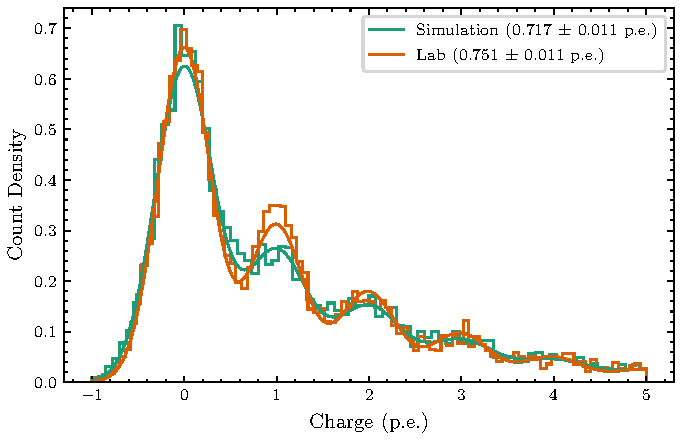
\includegraphics[width=\textwidth]{spe_sim_lab} 
	\caption[Comparison of the SPE spectra between lab measurements and simulations.]{Comparison of the SPE spectra for a single pixel between lab measurements and simulations after an initial attempt towards a more accurate Monte Carlo model. The SPE spectra were identically constructed in both cases, using the \textit{Cross Correlation} charge extraction method. Each spectra histogram was then fit using Equation~\ref{}. Three illuminations were simultaneously fit, however just a single illumination is displayed here. Both spectra are normalised in the x direction by their respective single-photoelectron value, and in the y direction such that their integral is 1.}
	\label{fig:spe_sim_lab}
\end{figure}

\final{reference spe fitting equation}

\begin{table}[h!]
\centering
\begin{tabular}{ll|ll} \toprule
    Fit Parameter        &            & Simulation          & Lab                \\ \midrule
    Average Illumination & [\si{\pe}] & 0.717 $\pm$ 0.011  & 0.751 $\pm$ 0.011 \\
    Pedestal Deviation   & [\si{\pe}] & 0.314 $\pm$ 0.003  & 0.286 $\pm$ 0.002 \\
    Gain Deviation       & [\si{\pe}] & 0.109 $\pm$ 0.009  & 0.078 $\pm$ 0.007 \\
    Optical Crosstalk    &            & 0.387 $\pm$ 0.007  & 0.350 $\pm$ 0.006 \\ \bottomrule
\end{tabular}
\caption{Parameter values resulting from the fit to the spectra in Figure~\ref{fig:spe_sim_lab}. The \si{1}{$\sigma$} parabolic errors obtained from the covariance matrix of the fit parameters are quoted.}
\label{table:spe_sim_lab}
\end{table}

For the simulation results presented in this thesis, an updated value was obtained for as many of the relevant \pkg{sim\_telarray} parameters as possible. Figure~\ref{fig:spe_sim_lab} displays the resulting differences in terms of the \gls{spe} spectra between lab and simulation. The discrepancies in parameters resulting from the fits to the \gls{spe} spectra are shown in Table~\ref{table:spe_sim_lab}, and are deemed to be close enough for the investigations in this thesis. Further details about the fit procedure for \gls{spe} spectra can be found in Appendix~\ref{a1-spe}. The differences between lab and simulation in other factors and at higher amplitudes are explored through \textit{Charge Resolution} comparisons, investigated later in this chapter.

\section{CHEC-S Charge Resolution}

The \textit{Charge Resolution} is the principle criterion used within \gls{cta} to express how well the camera can resolve a signal. The concept of \textit{Charge Resolution} is introduced in Section~\ref{section:cr}, alongside the \gls{cta} requirement \requirementref{B-TEL-1010 Charge Resolution}. It not only measures the quality of the camera's photosensor and electronics, but also the aptitude of the calibration and signal extraction. Consequently, obtaining a \textit{Charge Resolution} of the camera that meets this requirement has been the underlying driver behind my efforts in developing the techniques described in this thesis.

\subsection{Procedure and Datasets} \label{section:crprocedure}

As directed in the \requirementref{B-TEL-1010 Charge Resolution} requirement, one must simulate the response of the camera to Cherenkov shower illumination to verify the requirement is met. However, this result must be supported by evidence that the \textit{Charge Resolution} appropriately resembles the behaviour of the real camera. To achieve this, I display the \textit{Charge Resolution} with four different procedures. Each procedure bridges the gap between the \textit{Charge Resolution} I obtained with Cherenkov shower simulations, and the \textit{Charge Resolution} I obtained from lab measurements. The procedures, and their associated names for the purpose of this thesis, are:

\begin{description}
\item [Lab] Utilises uniform illumination datasets taken in the lab that cover the full dynamic range of the camera, with 1000 events at each illumination. The average expected charge per pixel (in photoelectrons) for each illumination is calibrated by the procedure detailed in Section~\ref{section:lab-calib}. Using the calibration procedures detailed in Chapter~\ref{ch5-calibration} and the \textit{Cross Correlation} charge extraction technique (Chapter~\ref{ch6-reduction}), a value of measured charge in photoelectrons is obtained for every waveform. As the average expected charge includes the Poisson fluctuations, it is appropriate to use Equation~\ref{eq:charge_res} for calculating the \textit{Charge Resolution}, with the measured charge per waveform used for ${Q_M}_i$ and the average expected charge for $Q_T$. It is important to note that these datasets are taken with no \gls{nsb} contribution, and are therefore not a completely appropriate measure against the \gls{cta} requirement (defined for an \gls{nsb} photon rate per pixel of $\SI{0.125}{\pe/ns} = \SI{125}{MHz}$). However, a \gls{dcr} of \SI{\sim5}{MHz} is assumed to be present in the \gls{sipmt}.
\item [MCLab] Simulations of the dynamic range datasets from the lab are obtained with the updated \pkg{sim\_telarray} camera model. Using the identical method used for the lab data (excluding the \gls{target} calibration) the charge is extracted and calibrated from the waveforms. The average expected charge for each illumination per pixel is also obtained in the same way as the previous procedure. However, the simulations contain perfect laser uniformity across the camera face (though the geometry corrections shown in Section~\ref{section:illumination_profile} are still applicable, as the simulations contain a point source \SI{\sim 1.5}{m} from the camera). This dataset then fully represents the same measurements, but with the Monte Carlo model of the camera instead of the physical camera. With an accurate model of the camera, the \textit{Charge Resolution} result should be the same as from the lab measurements. Equation~\ref{eq:charge_res} is also used in this procedure for calculating the \textit{Charge Resolution}.
\item [MCLabTrue] Utilises the same dataset as the previous procedure, but instead of using the average expected charge, the true number of photoelectrons that were incident on the pixel for each waveform are extracted from the simulation file. The linear fit between the average measured charge and the ``true charge'' is used to calibrate the extracted charge into corresponding units. As the unique value of ``true charge'' per waveform is now used as $Q_T$, Equation~\ref{eq:charge_res2} must be used to account for the lack of Poisson fluctuations in $Q_T$. The \textit{Charge Resolution} resulting from this procedure demonstrates the change in transitioning from ``average expected charge'' to ``true charge'', which is important for interpreting the results from the next procedure.
\item [MCOnsky] Produced using a dataset containing Monte Carlo simulations of gamma-ray-induced air shower observations is created using \pkg{CORSIKA} and \pkg{sim\_telarray}. A model of \gls{chec-s} on the \gls{astri} telescope structure is used in the simulation. The \textit{Charge Resolution} is then calculated with the same procedure as in \textit{MCLabTrue}. As only a small section of the camera is illuminated by the Cherenkov camera, this procedure is dependant on the peak-finding methods described in Chapter~\ref{ch6-reduction}. The \textit{Local Peak Finding} technique is used for this investigation. This \textit{Charge Resolution} procedure is the definitive approach for assessment of \textit{Charge Resolution}, as defined in the requirement. The previous procedures exist to support the claim that this result is applicable to the real camera.
\end{description}

\subsection{Lab Results}

\begin{figure}
	\centering
    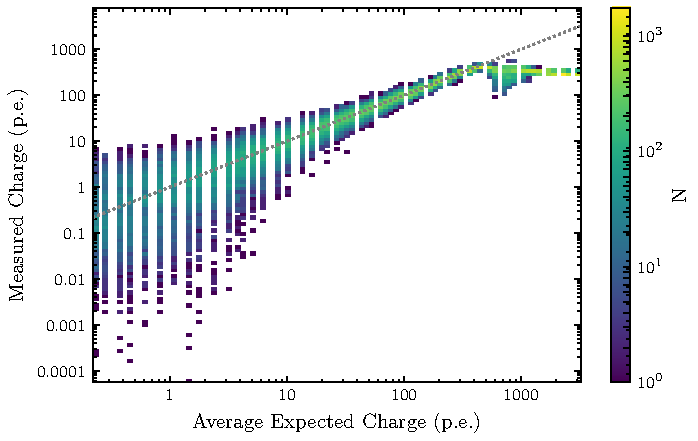
\includegraphics[width=\textwidth]{checs_mve_hist} 
	\caption[CHEC-S measured charge versus average expected charge.]{Two-dimensional histogram showing every measured charge for a single CHEC-S pixel, covering the full dynamic range. This dataset matches the one described in the \textit{Lab} procedure in Section~\ref{section:crprocedure}. The grey dotted line represents a one-to-one relation between the axes.}
	\label{fig:checs_mve_hist}
\end{figure}

\begin{figure}
	\centering
    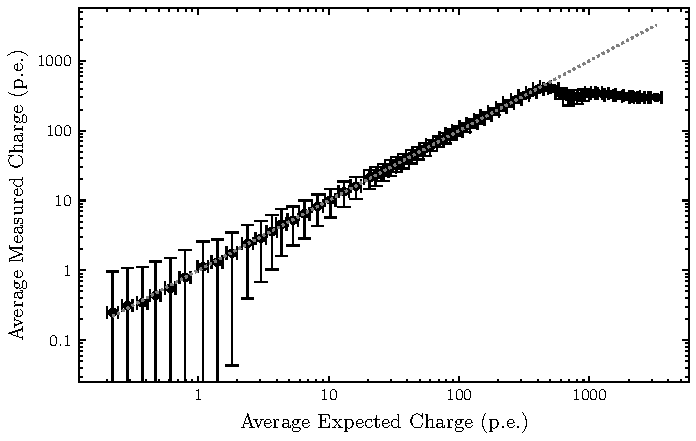
\includegraphics[width=\textwidth]{checs_mve_scatter} 
	\caption[CHEC-S average measured charge versus average expected charge.]{Similar to Figure~\ref{fig:checs_mve_hist}, but summarising the entries in terms of their averages and standard deviation for each illumination. The X error bars represent the uncertainty in the filter-wheel calibration into units of \si{\pe} (Section~\ref{section:fwerr}).}
	\label{fig:checs_mve_scatter}
\end{figure}

\begin{figure}
	\centering
    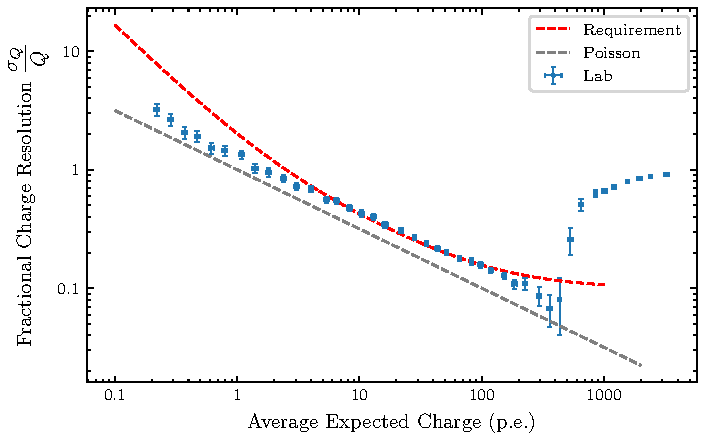
\includegraphics[width=0.9\textwidth]{cr_1_lab_raw} 
	\caption[\textit{Charge Resolution} of the Lab dataset in default units.]{Average \textit{Charge Resolution} across CHEC-S (excluding ``dead'' pixels) for the same Lab dynamic range dataset Figure~\ref{fig:checs_mve_hist} uses. The Y error bars represent the standard deviation of the \textit{Charge Resolution} values across the camera. The X error bars represent the uncertainty in the filter-wheel calibration into units of \si{\pe} (Section~\ref{section:fwerr}). The points are binned to improve visibility. The presentation of the \textit{Charge Resolution} in this form matches Figure~\ref{fig:charge_res_req}.}
	\label{fig:cr_1_lab_raw}
\end{figure}

\begin{figure}
	\centering
    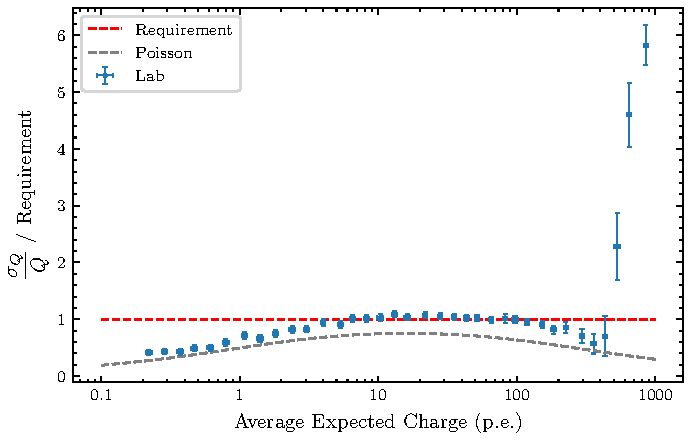
\includegraphics[width=0.9\textwidth]{cr_1_lab} 
	\caption[\textit{Charge Resolution} of the Lab dataset with respect to the requirement.]{Same result shown in Figure~\ref{fig:cr_1_lab_raw}, but with respect to the requirement curve to emphasise the separation between it and the points.}
	\label{fig:cr_1_lab}
\end{figure}

To begin, the different representations of the \textit{Charge Resolution} are first explained in terms of the \textit{Lab} procedure and dataset. Figure~\ref{fig:checs_mve_hist} demonstrates the charge extracted for the entire dynamic range dataset, post calibration. It is the purpose of the \textit{Charge Resolution} to consolidate the spread and bias of these measured charges (from the average expected charge) into a single value per average expected charge (or ``true charge'' where appropriate). The average measured charges in Figure~\ref{fig:checs_mve_scatter} seem to strongly follow a one-to-one relation with the average expected charge (in the non-saturated region), attesting to the success of the extracted charge calibration. However, to fully explore the performance of the camera, we continue on to the \textit{Charge Resolution} shown in Figure~\ref{fig:cr_1_lab_raw}. It is immediately obvious that in the saturated region (\SI{> 300}{\pe}), the camera fails the \textit{Charge Resolution} requirement. This is expected, as we make no attempt to recover saturated signals in this investigation. Methods to account for the saturation are briefly described in Section~\ref{section:saturation}, and will be fully explored in a future investigation. 

To investigate other less obvious features in the \textit{Charge Resolution}, I display the \textit{Charge Resolution} in terms of its deviation from the requirement curve. This is achieved by dividing the \textit{Charge Resolution} curve by the requirement curve. Figure~\ref{fig:cr_1_lab} expresses the \textit{Charge Resolution} from Figure~\ref{fig:cr_1_lab_raw} in this format. This is how the \textit{Charge Resolution} is visualised elsewhere in this thesis, as it shows how close the points are to the requirement, and emphasises features that cause the results to fail the requirement. In the region of $10 < Q_\text{Exp} < 100$~\si{\pe}, the \textit{Charge Resolution} of the \textit{Lab} dataset is above the requirement curve, and therefore fails the requirement. By comparing this \textit{Charge Resolution} to those resulting from different Monte Carlo simulations that explore the contributing parameter space, we are able to identify the primary factors resulting in a failure to meet the requirement.

\subsection{Lab versus Monte Carlo}

As a preface to the simulated \textit{Charge Resolution} investigations, the differences in the results of the procedures described in Section~\ref{section:crprocedure} are illustrated in Figure~\ref{fig:cr_2_lab_vs_mc}. The earlier descriptions of each procedure indicate the following expected differences between their \textit{Charge Resolutions}:
\begin{itemize}
\item With a perfect Monte Carlo model of the camera, there should be no differences between the \textit{Charge Resolution} of \textit{Lab} and \textit{MCLab}. Any deviations arise from a misunderstanding in the camera's behaviour, or from an unaccounted noise contribution.
\item The difference between \textit{MCLab} and \textit{MCLabTrue} demonstrates the expected change when transitioning from the average expected charge, to the ``true charge'' that was detected in the pixel.
\item As they are the same camera model, and the same \textit{Charge Resolution} calculation approach, there should be very little difference between \textit{MCLabTrue} and \textit{MCOnsky}. The only factor to contribute to differences between the two procedures is the peak-finding that is necessary for the \textit{MCOnsky} datasets.
\end{itemize}

\begin{figure}[H]
	\centering
    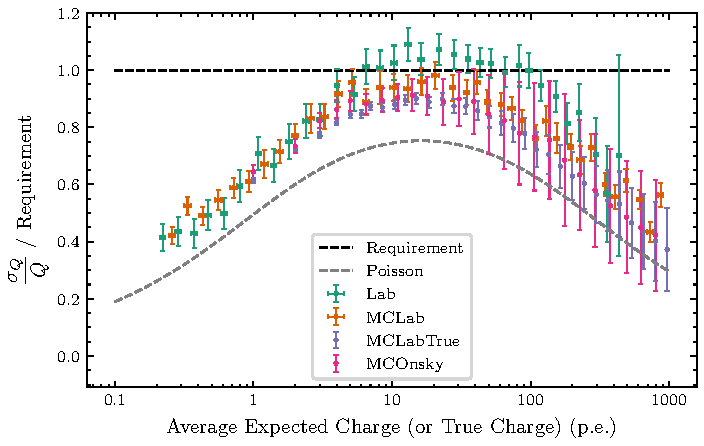
\includegraphics[width=\textwidth]{cr_2_lab_vs_mc} 
	\caption[Comparison of the different \textit{Charge Resolution} procedures.]{Comparison of the \textit{Charge Resolutions} resulting from the different procedures described in Section~\ref{section:crprocedure}. A background photon rate of \SI{5}{MHz} is simulated in the Monte Carlo datasets to represent the \gls{dcr} we expect inside the datasets produced from lab measurements. The saturated points from the \textit{Lab} measurements are outside of the figure's range.}
	\label{fig:cr_2_lab_vs_mc}
\end{figure}

It is therefore apparent in Figure~\ref{fig:cr_2_lab_vs_mc} that our simulation model is not a perfect representation of \gls{chec-s}. The lack of saturation in the simulated datasets is expected, and that is a feature we will include in future investigations. However, from the simulated datasets we can conclude that in the absence of additional \gls{nsb} photons, the \textit{Charge Resolution} of our camera before the saturated region should be below the requirement. As we do not observe this in the non-simulated dataset, there must be a noise contribution we have not appropriately accounted for. The work required to fully diagnose this noise contribution is beyond the scope of this thesis; however, possible options include:
\begin{description}
\item [Transfer Functions] The simulations do not fully simulate the \gls{chec-s} electronics. They contain no resemblance of the digitising behaviour of \gls{target} \glspl{asic}, and therefore no variations in amplitude response exists from sample-to-sample. Inaccuracies in the Transfer Function calibration (Chapter~\ref{ch5-calibration}) could manifest themselves as differences between the \textit{Charge Resolutions} of lab and simulated data.
\item [Timing] As mentioned in Section~\ref{section:timing_corrections}, the variations in signal arrival time between pixels could degrade the \textit{Charge Resolution}. This contribution is not included in the simulation.
\item [Electrical Crosstalk] Inside the simulation, each pixel is considered independently. Due to electronic coupling, this is unfortunately not the case in reality. \change{Rich: better description (technical) of how the electronic crosstalk happens, e.g. of ground bounce}
\item [Optical Crosstalk] A simplified form of optical crosstalk is used in the simulation, via the input \gls{spe} spectra shape. This may not fully characterise the full behaviour of the optical crosstalk.
\item [Reference Pulse Shape] Another major difference between simulation and reality is the behaviour of the pulse shape. In simulations, the pulse shape at all illuminations is constructed by the superposition of the individual photoelectron pulses. If that description was appropriate for the real camera, the pulse shape dependency with amplitude would not be seen in Section~\ref{section:pulse_shape_results}. As we use the \textit{Cross Correlation} charge extraction method, the measured charge is sensitive to changes in pulse shape. This could, in theory, result in discrepancies between the \textit{Charge Resolutions} of lab and simulated data. However, the investigations in Appendix~\ref{a3-extractors} seem to suggest this factor is not significant.
\end{description}

Identifying the cause of this noise contribution is of paramount importance in the commissioning of \gls{chec-s}. However, the remainder of this section will explore the possibility of meeting the \textit{Charge Resolution} even in the presence of this unknown noise contribution. This procedure may give insight into the source of the noise.

\subsection{Night Sky Background}

\begin{figure}[H]
	\centering
    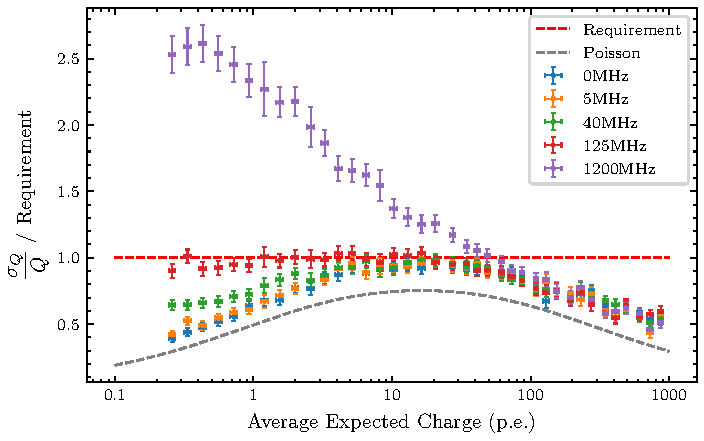
\includegraphics[width=\textwidth]{cr_3_nsb_comparison_mclab} 
	\caption[Comparison of the \textit{Charge Resolution} at different NSBs.]{Comparison of the \textit{Charge Resolutions} obtained from the \textit{MCLab} procedure when simulating different Night Sky Background (NSB) photon rates.}
	\label{fig:cr_3_nsb_comparison_mclab}
\end{figure}

As the \gls{nsb} photon rate increases, we expect more noise to be included in the charge extraction. This results in a higher charge then expected, and increases the variation in signal measured for the same average illumination. Figure~\ref{fig:cr_3_nsb_comparison_mclab} illustrates the degradation in charge resolution caused by an increase in \gls{nsb} rate. The effects are most pronounced at the lower values of average expected charge, where an increase in \gls{nsb} has a larger impact on the signal-to-noise ratio. We can conclude from this figure that even if the unknown noise contribution in the \textit{Lab} datasets is corrected for, the current design of \gls{chec-s} could potentially fail to meet the \gls{cta} requirement at the specified \gls{nsb} of \SI{125}{MHz}.

\begin{figure}
	\centering
    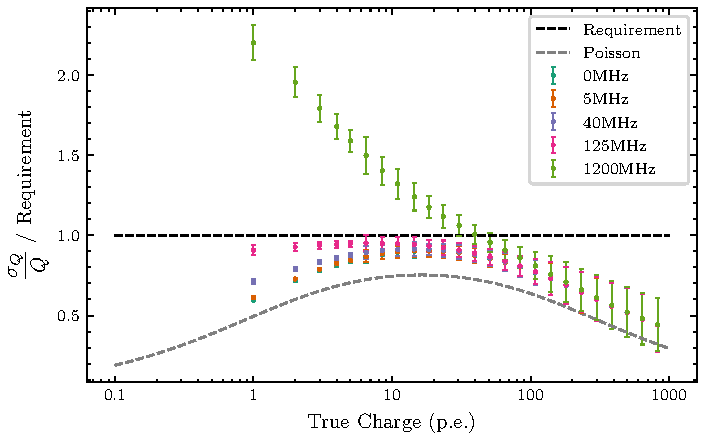
\includegraphics[width=\textwidth]{cr_3_nsb_comparison_mclabtrue} 
	\caption[Comparison of the \textit{Charge Resolution} at different NSBs using the \textit{MCLabTrue} procedure.]{Comparison of the \textit{Charge Resolutions} obtained from the \textit{MCLabTrue} procedure when simulating different values of NSB.}
	\label{fig:cr_3_nsb_comparison_mclabtrue}
\end{figure}

A similar dependence on \gls{nsb} is observed with the \textit{MCLabTrue} procedure in Figure~\ref{fig:cr_3_nsb_comparison_mclabtrue}, however the \textit{Charge Resolutions} demonstrate an overall improved performance over the \textit{MCLab} representation (Figure~\ref{fig:cr_3_nsb_comparison_mclab}).

\begin{figure}
	\centering
    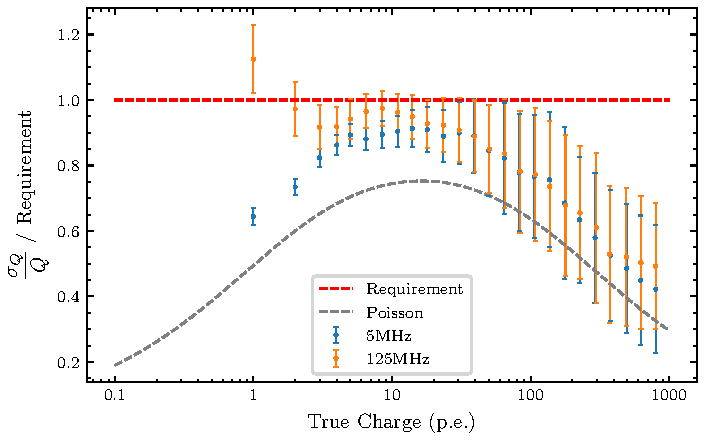
\includegraphics[width=\textwidth]{cr_3_nsb_comparison_mconsky} 
	\caption[Comparison of the \textit{Charge Resolution} at two different NSBs when observing Cherenkov showers (via the\textit{MCOnsky} procedure).]{Comparison of the \textit{Charge Resolutions} obtained from simulated observations of Cherenkov showers (via the \textit{MCOnsky} procedure), when simulating different values of NSB. The signal inside each waveform is found with the \textit{Local Peak Finding} approach.}
	\label{fig:cr_3_nsb_comparison_mconsky}
\end{figure}

Despite the improved performance achieved when using the ``true charge'', a second consequence of higher \gls{nsb} is the increased difficulty of finding the signal pulse among the noise pulses. As shown in Figure~\ref{fig:cr_3_nsb_comparison_mconsky}, this causes the current model of \gls{chec-s} to fail the \textit{Charge Resolution} requirement when observing Cherenkov showers. An alternative to the \textit{Local Peak Finding} approach could improve on this bias to noise pulses, and therefore enable the requirement to be met.

\subsection{Optical Crosstalk}

\begin{figure}[H]
	\centering
    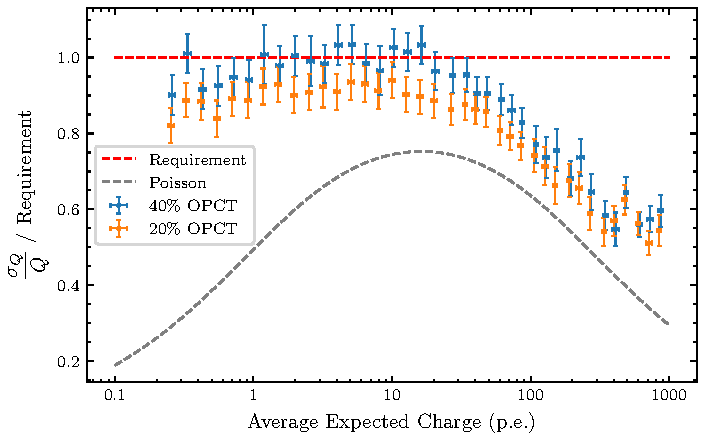
\includegraphics[width=\textwidth]{cr_4_opct_mc} 
	\caption[Comparison of the \textit{Charge Resolution} at different values of optical crosstalk.]{Comparison of the \textit{Charge Resolutions} obtained from the \textit{MCLab} procedure when simulating different values of optical crosstalk (abbreviated here as OPCT). An \gls{nsb} rate of \SI{125}{MHz} was included in these simulations.}
	\label{fig:cr_4_opct_mc}
\end{figure}

A prime suspect for the poor \textit{Charge Resolution} is the very high (\SIrange{35}{40}{\percent}) optical crosstalk in the \glspl{sipmt} currently used for the \gls{chec-s} prototype. The optical crosstalk contributes to the extracted charge in two ways: 
\begin{itemize}
\item The measured charge is consistently higher. This factor is accounted for in the flat-fielding calibration (Section~\ref{section:photosensor_calib}).
\item The spread in charge that results from a particular amount of photons contains a higher variation. This is therefore expressed as an increase in the \glsf{enf} (see Section~\ref{section:sipmts}).
\end{itemize}

\subsubsection{Monte Carlo}

Figure~\ref{fig:cr_4_opct_mc} demonstrates the \textit{MCLab Charge Resolution} for a simulation of the \gls{chec-s} model, but with \SI{20}{\percent} optical crosstalk. This is compared to the original model with \SI{40}{\percent} optical crosstalk. The effect of a reduced optical crosstalk in the simulation is an improvement in the \textit{Charge Resolution} for all illuminations.

\begin{figure}[H]
	\centering
    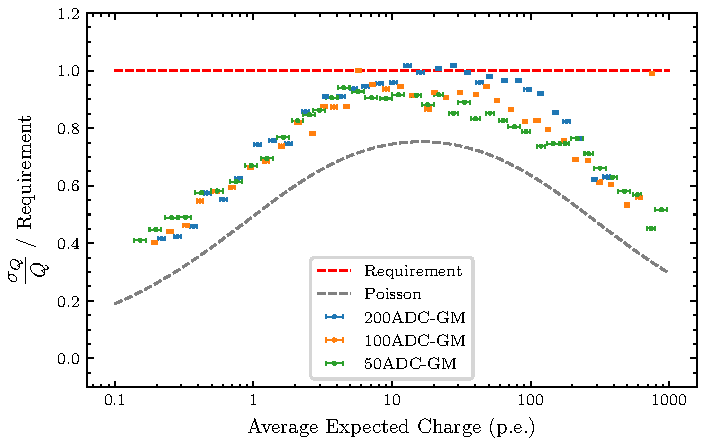
\includegraphics[width=\textwidth]{cr_4_opct_biasvoltage} 
	\caption[Comparison of the \textit{Lab Charge Resolution} with different bias voltages applied to the SiPM pixel.]{Comparison of the \textit{Charge Resolutions} obtained from different \textit{Lab} datasets. Each dataset is gain-matched to a different ADC value. By gain matching to different ADC values, a different bias voltage is applied to the \gls{sipmt} pixel. As this dataset was gain-matched in units of ADC, the spread between pixels is large. Therefore, only a single pixel's \textit{Charge Resolution} is shown.}
	\label{fig:cr_4_opct_biasvoltage}
\end{figure}

\begin{table}[h!]
\centering
\begin{tabular}{ll|lll} \toprule
    Fit Parameter          &             & \SI{200}{ADC}     & \SI{100}{ADC}     & \SI{50}{ADC}      \\ \midrule
    Average Illumination 1 & [\si{\pe}]  & 1.061 $\pm$ 0.014 & 0.903 $\pm$ 0.023 & 0.550 $\pm$ 0.009 \\
    Average Illumination 2 & [\si{\pe}]  & 0.793 $\pm$ 0.012 & 0.688 $\pm$ 0.021 & 0.394 $\pm$ 0.008 \\
    Average Illumination 3 & [\si{\pe}]  & 0.625 $\pm$ 0.010 & 0.535 $\pm$ 0.014 & 0.301 $\pm$ 0.007 \\

    Pedestal Deviation     & [\si{mVns}] & 6.047 $\pm$ 0.043 & 5.668 $\pm$ 0.049 & 5.913 $\pm$ 0.039 \\
    Gain                   & [\si{mVns}] & 21.33 $\pm$ 0.073 & 16.06 $\pm$ 0.108 & 12.10 $\pm$ 0.094 \\
    Gain Deviation         & [\si{mVns}] & 1.684 $\pm$ 0.159 & 0.005 $\pm$ 15.03 & 0.003 $\pm$ 11.05 \\
    Optical Crosstalk      &             & 0.339 $\pm$ 0.006 & 0.242 $\pm$ 0.011 & 0.100 $\pm$ 0.006 \\ \bottomrule
\end{tabular}
\caption{Parameter values resulting from the fit to the SPE spectra of the different gain-matched datasets for a single pixel. Three illuminations were simultaneously fit. These three illuminations are identical in terms of filter-wheel transmission (and therefore average photons) between the three gain-matched datasets.}
\label{table:spe_gm}
\end{table}

\subsubsection{Changing Bias Voltage}

Due to the dependence of the optical crosstalk on the overvoltage across the \gls{sipmt} (described in Section~\ref{section:sipmt_parameters}), it is possible to investigate the impact a reduced optical crosstalk has on \textit{Charge Resolution} using \textit{Lab} data that is taken with different bias voltages. Three datasets were generated, each gain-matched to a different ADC value (the Transfer Functions were not included in the gain matching procedure at the time). The \SI{200}{ADC} gain-matched dataset is at a similar bias voltage to the the dataset in Figure~\ref{fig:cr_1_lab}. The \SI{100}{ADC} and \SI{50}{ADC} gain-matched datasets are produced by reducing the bias voltage. The effect of a reduced bias voltage on the \gls{sipmt} characteristics is quantified in the parameters extracted from the fit to the \gls{spe} spectra, shown in Table~\ref{table:spe_gm}. In total, the optical crosstalk is reduced by a factor of 3 to \SI{10}{\percent} in going from a gain matching of \SI{200}{ADC} to \SI{50}{ADC}.

Figure~\ref{fig:cr_4_opct_biasvoltage} shows the improvement in \textit{Charge Resolution} with reduced bias voltage, bringing the result below the requirement. Additionally, by reducing the bias voltage, the unexplained noise component that was identified in the comparison between the \textit{Lab} and \textit{MCLab} datasets (Figure~\ref{fig:cr_2_lab_vs_mc}) appears to diminish, suggesting it is possibly related to the optical crosstalk.

However, it is important to note that by reducing the bias voltage, we also decrease the \glsf{pde} of the \gls{sipmt} (Figure~\ref{fig:sipmt_checs}). This effect is evident in the average illumination values quoted in Table~\ref{table:spe_gm}. The result of a lower \gls{pde} is a reduction in the camera's ability to detect Cherenkov shower photons. This contradiction between improving \textit{Charge Resolution}, but reducing Cherenkov shower resolution, is one of the primary reasons the \gls{cta} requirements are being redefined to be in terms of photons, as described in Chapter~\ref{ch3-architecture}.

\subsection{Analytical Description}

One further way to characterise the camera's \textit{Charge Resolution} is to use the analytical description of the \textit{Charge Resolution} provided by Equation~\ref{eq:charge_res_req}. However, to fully interpret this function, we must understand the contribution of optical crosstalk to the $\sigma_{ENF}$ parameter. If we assume that optical crosstalk is the dominant contributor to $\sigma_{ENF}$ for an \gls{sipmt} (a reasonable assumption due to its high \gls{spe} resolution), the following equations derived by \textcite{Vinogradov2012} can be used to express the $\sigma_{ENF}$ in terms of the optical crosstalk probability $P_\text{opct}$:
\begin{minipage}{\textwidth}
\begin{equation} \label{eq:opct_geometric}
\sigma_{ENF} \approx 1 + P_\text{opct},
\end{equation}
\begin{equation} \label{eq:opct_branching}
\sigma_{ENF} \approx 1 + P_\text{opct} + \frac{3}{2} P_\text{opct}^2,
\end{equation}
\end{minipage}
where the former equation is applicable in a geometric chain model of the optical crosstalk behaviour (each single electron response is capable of only producing 1~or~0 further electron responses) and the latter equation is applicable in a branching Poisson model (each single electron response produces a Poisson distributed random number of further electron responses). The $P_\text{opct}^3$ term from the equation derived by \textcite{Vinogradov2012} is assumed to be negligible.

\begin{figure}[h]
	\centering
    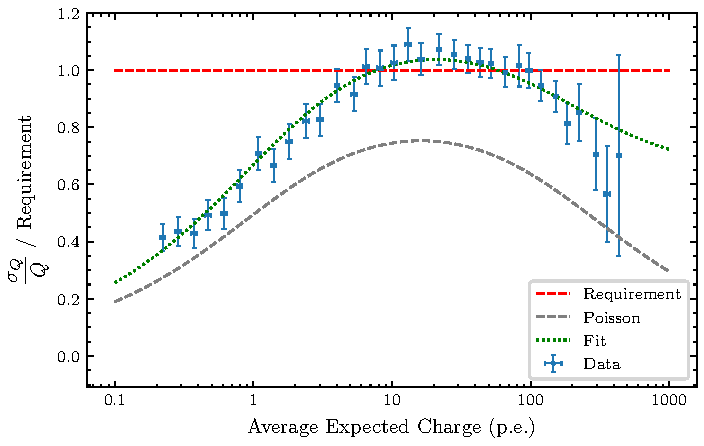
\includegraphics[width=\textwidth]{cr_7_fit} 
	\caption[Analytical fit of the \textit{Lab Charge Resolution}.]{Analytical fit of the \textit{Lab Charge Resolution} using Equation~\ref{eq:charge_res_req}. All ``non-dead'' pixels are included in the fit to give the an average characterisation of the whole camera. The fit result is used to predict the \textit{Lab Charge Resolution} at \SI{125}{MHz} \gls{nsb}, and then with \SI{10}{\percent} optical crosstalk in the presence of \SI{125}{MHz} \gls{nsb}. The possible relationships between \gls{enf} and optical crosstalk are shown in Equations~\ref{eq:opct_geometric}~and~\ref{eq:opct_branching}.}
	\label{fig:cr_7_fit}
\end{figure}

\begin{table}[h]
\centering
\begin{tabular}{ll|ll} \toprule
    Fit Parameter        &                & Values             \\ \midrule
    Background Noise     & $\sigma_0$     & 0.000 $\pm$ 0.316  \\
    Excess Noise Factor  & $\sigma_{ENF}$ & 1.338 $\pm$ 0.003  \\
    Miscalibration       & $\sigma_g$     & 0.067 $\pm$ 0.001  \\ \bottomrule
\end{tabular}
\caption{Parameter values resulting from the fit to the \textit{Lab Charge Resolution} (Figure~\ref{fig:cr_7_fit}) using Equation~\ref{eq:charge_res_req}.}
\label{table:cr_7_fit}
\end{table}

Shown in Figure~\ref{fig:cr_7_fit} is the result from fitting Equation~\ref{eq:charge_res_req} to the \textit{Lab Charge Resolution} from Figure~\ref{fig:cr_1_lab}. The resulting parameters, shown in Table~\ref{table:cr_7_fit}, indicate that $\sigma_0$ was poorly constrained by the data points, however $\sigma_{ENF}$ and $\sigma_g$ are well characterised. The first conclusion provided by the fit is the miscalibration is very low, and is potentially still overestimated due to the lack of high charge measurements (values above the saturation point were excluded). Secondly, using Equations~\ref{eq:opct_geometric}~and~\ref{eq:opct_branching}, the measured \gls{enf} suggests either an optical crosstalk of \SI{34}{\percent} (geometric) or \SI{25}{\percent} (branching Poisson) for the camera. If the same parameters are used in combination with a value for $\sigma_0$ calculated using Equation~\ref{eq:charge_res_nsb} and values $\mathit{NSB} = \SI{125}{MHz}$, $t_w = \SI{15}{ns}$, and $n_e = 0.3$, we can once again conclude that the \textit{Charge Resolution} requirement is failed by the current \gls{chec-s} design. The curve resulting from this extrapolation is shown in Figure~\ref{fig:cr_7_fit} labelled as ``\SI{125}{MHz}''.

\subsection{Conclusion}

The results of these \textit{Charge Resolution} investigations seem to suggest the optical crosstalk is the dominating factor in the degradation of the \textit{Charge Resolution} performance for \gls{chec-s}. They also show that a reduction in optical crosstalk could allow \gls{chec-s} to meet the \textit{Charge Resolution} requirement. Such a reduction is possible with newer \glspl{sipmt}, which use techniques such as ``trenching'' to reduce the optical crosstalk between microcells. This is discussed in more detail in Section~\ref{section:checs_future}. Within this year, a second \gls{chec-s} prototype will be built using the latest \glspl{sipmt}, which are reported to have an optical crosstalk of \SI{\sim 10}{\percent}. If we once again use the result of the fit from Figure~\ref{fig:cr_7_fit}, we can predict the \textit{Charge Resolution} performance of this future camera under \SI{125}{MHz} \gls{nsb}. This is shown in the curves ``\SI{10}{\percent} OPCT (Geometry)'' and ``\SI{10}{\percent} OPCT (Branching)'', and concludes that such a camera will safely meet the \textit{Charge Resolution} requirement.

\section{CHEC-S Pulse Shape} \label{section:pulse_shape_results}

\begin{figure}
	\centering
    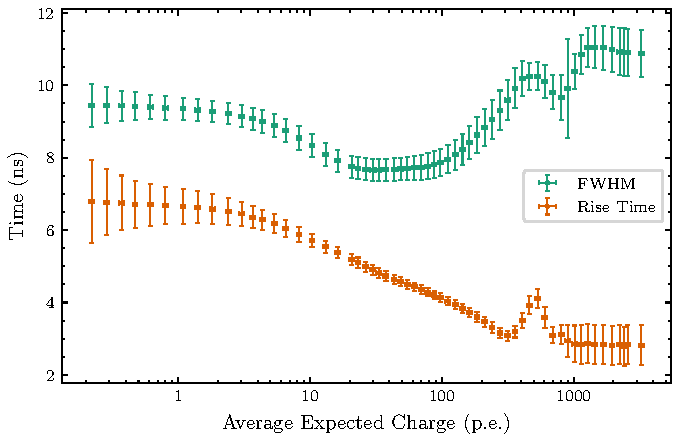
\includegraphics[width=\textwidth]{pulse_shape_lab} 
	\caption[Pulse shape versus average expected charge for CHEC-S.]{The average pulse shape across CHEC-S as a function of average expected charge (i.e. illumination). The Y errors are the standard deviation of the pulse shape parameters across the camera. The ``dead'' pixels are excluded from the calculation.}
	\label{fig:pulse_shape_lab}
\end{figure}

\begin{figure}
	\centering
    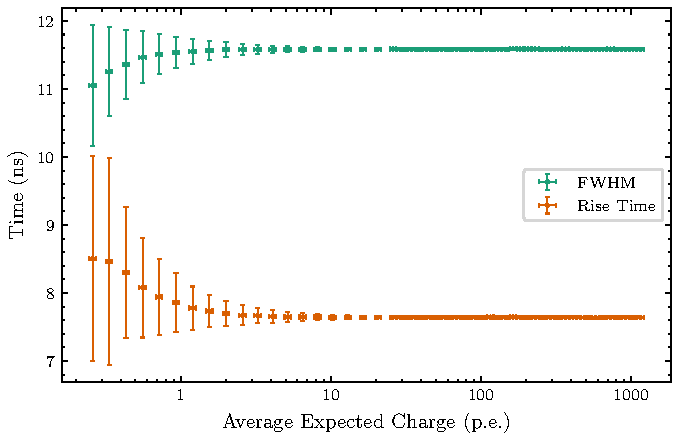
\includegraphics[width=\textwidth]{pulse_shape_mc} 
	\caption[Pulse shape versus average expected charge for a CHEC-S simulation.]{The average pulse shape extracted using data obtained from simulations of \gls{chec-s}. The processing and representation is identical to those used in Figure~\ref{fig:pulse_shape_lab}. An \gls{nsb} photon rate of \SI{5}{MHz} is included to imitate the expected \gls{dcr} contained in the measurements from the real camera.}
	\label{fig:pulse_shape_mc}
\end{figure}

Although there is no \gls{cta} requirement attached directly to it, the pulse shape of the camera is important to understand. The pulse shape behaviour influences the performance of the charge extraction, especially when using methods that utilise the expected shape of the pulse, such as a fitting technique, or the \textit{Cross Correlation} method. Figure~\ref{fig:pulse_shape_lab} displays the average pulse shape of \gls{chec-s} in terms of the pulse's FWHM and rise time. The FWHM is defined as the width of the pulse at half of its maximum. The rise time is the time between \SI{10}{\percent} of the pulse maximum, to \SI{90}{\percent}. A perfect detector should have a consistent pulse shape at all illuminations, as shown with the simulation dataset in Figure~\ref{fig:pulse_shape_mc}. The only deviations from a constant pulse shape in the simulation dataset is at low illuminations, where the noise makes it harder to characterise the pulse. 

It is suspect that the region in which the FWHM appears to drop in Figure~\ref{fig:pulse_shape_lab} ($10 < Q_\text{Exp} < 100$~\si{\pe}) coincides with the same region where we see the discrepancy between the \textit{Lab} and \textit{MCLab Charge Resolutions} (Figure~\ref{fig:cr_2_lab_vs_mc}). This suggests the two factors could be correlated. Further investigation into the pulse shape behaviour is required, possibly by probing at different points in the \gls{fee} to observe each components effect on the pulse shape. 

\section{CHEC-S Time Resolution}

\begin{figure}
	\centering
    \includegraphics[width=\textwidth]{checs_time_resolution} 
	\caption[CHEC-S \textit{Time Resolution}.]{The \textit{Time Resolution} of the CHEC-S prototype, compared against the \textit{Time Resolution} from simulations of CHEC-S. The points represent the average \textit{Time Resolution} across 100 events, while the Y error bars indicate the standard deviation across 100 events. The X error bars are the uncertainty in the average expected charge.}
	\label{fig:checs_time_resolution}
\end{figure}

A further criterion for assessing a camera's behaviour within \gls{cta} is the \textit{Time Resolution}. Introduced in Section~\ref{section:time_res}, the \textit{Time Resolution} is a measure of how the pulse time varies between pixels. After applying the timing corrections for each pixel (Section~\ref{section:timing_corrections}), the \textit{Time Resolution} $\sigma_T$ for an event is calculated using Equation~\ref{eq:time_res}. Only pixels with a measured charge greater that \SI{5}{\pe} are included in the calculation. The mean and standard deviation of $\sigma_T$ across multiple events is then expressed against the average expected charge as shown in Figure~\ref{fig:checs_time_resolution}. In order to meet the \gls{cta} requirement, the \textit{Time Resolution} must remain below the requirement at all values of average expected charge.

While the curve for the real \gls{chec-s} prototype appears to meet the requirement in Figure~\ref{fig:checs_time_resolution}, the dataset used contained no \gls{nsb} photons (only an assumed \gls{dcr} of \SI{5}{MHz}. Therefore, for extrapolation purposes, the \textit{Time Resolution} extracted from a simulation at an \gls{nsb} photon rate of \SI{5}{MHz}, and a second simulation at a rate of \SI{125}{MHz}, was included alongside the result from the real camera.

The pulse time extraction method used in this investigation was to select the maximum sample within a \SI{14}{ns} window around the maximum of the average waveform across all pixels. This technique is very simple and highly influenced by to sample-to-sample variations. It is therefore no surprise that the camera appears to fail the \textit{Time Resolution} requirement at high \gls{nsb} photon rates. As outlined in the requirement, the method used to extract the pulse time for the calculation of \textit{Time Resolution} does not need to be the same method used for charge extraction. Therefore a more advanced method, such as fitting the pulse, could be used to improve the resolution, and meet the requirement.

A further conclusion that may be drawn from Figure~\ref{fig:checs_time_resolution} is that the real ``Lab'' camera does exhibit some additional time variations from pixel-to-pixel due to the electronics, which are not present in the simulation. This is the cause of the discrepancy between the ``Lab'' and ``Simulation'' curves at high illuminations. At lower illuminations however, the sample-to-sample noise is the dominating factor, resulting in a more similar behaviour between the two curves.

\section{CHEC-M}

\begin{figure}
	\centering
    \includegraphics[width=\textwidth]{checm_mve_scatter} 
	\caption[CHEC-M average measured charge versus average expected charge.]{The dynamic range for a single CHEC-M pixel. Equivalent to Figure~\ref{fig:checs_mve_scatter}, but for CHEC-M.}
	\label{fig:checm_mve_scatter}
\end{figure}

Earlier studies of mine, that were concerned with the performance of \gls{chec-m}, have previously been included in a publication on \gls{chec-m} by \textcite{Zorn2017}. However, the calibration procedures have improved since that publication (hereby referred to as the ``CHEC-M paper''), and an investigation into the \textit{Charge Resolution} was not previously performed. A brief update regarding the performance of \gls{chec-m} is therefore included here, using the same techniques developed for \gls{chec-s}, while relying on the same dataset used to produce the figures in the CHEC-M paper.

Firstly, an updated version of the dynamic range plot (Figure~15 in the \mbox{CHEC-M} paper) is shown in Figure~\ref{fig:checm_mve_scatter}. By utilising similar techniques described in Section~\ref{section:lab-calib}, the understanding of the filter wheel's behaviour (as it existed at the time this data was taken) was improved. This is reflected in the new positions of the points on the X axis, and the larger error bars which more appropriately represent the uncertainty in the calibration.

\begin{figure}
	\centering
    \includegraphics[width=\textwidth]{cr_5_camera_comparison} 
	\caption[\textit{Charge Resolution} of CHEC-M.]{\textit{Charge Resolution} of CHEC-M compared to the \textit{Charge Resolution} of CHEC-S. The fit to the CHEC-M \textit{Charge Resolution} using Equation~\ref{eq:charge_res_req} is also shown.}
	\label{fig:cr_5_camera_comparison}
\end{figure}

\begin{table}[h!]
\centering
\begin{tabular}{ll|ll} \toprule
    Fit Parameter        &                & Values             \\ \midrule
    Background Noise     & $\sigma_0$     & 0.814 $\pm$ 0.007  \\
    Excess Noise Factor  & $\sigma_{ENF}$ & 1.642 $\pm$ 0.008  \\
    Miscalibration       & $\sigma_g$     & 0.073 $\pm$ 0.003  \\ \bottomrule
\end{tabular}
\caption{Parameter values resulting from the fit to the CHEC-M \textit{Charge Resolution} (Figure~\ref{fig:cr_5_camera_comparison}) using Equation~\ref{eq:charge_res_req}.}
\label{table:cr_5_camera_comparison}
\end{table}

Resulting from the dynamic range measurements, the \textit{Charge Resolution} of \gls{chec-m} can be constructed. This is shown in Figure~\ref{fig:cr_5_camera_comparison}, compared against the \textit{Lab Charge Resolution} of \gls{chec-s}, and the fit of Equation~\ref{eq:charge_res_req} to the \gls{chec-m} points. The parameters resulting from the fit are shown in Table~\ref{table:cr_5_camera_comparison}. While the \glspl{mapmt} of \gls{chec-m} do not suffer from the large optical crosstalk found in the \glspl{sipmt} of \gls{chec-s}, \gls{chec-m} does seem to still have a larger \gls{enf}. This is one justification for the choice of \gls{chec-s} over \gls{chec-m}.
%    \chapter{\label{ch8-onsky}On-Sky Observations} 

\minitoc

\notes[inline,caption={}]{
	\section{Plan}
	\subsection{Topics}
	\begin{itemize}
		\item Decided upon reduction methods
		\item Potentially different than for performance chapter
		\item CHEC-M campaign
		\item MC CHEC-S
		\item Future observations
		\item Jupiter observations (Beyond cherenkov?)
	\end{itemize}
	\subsection{Questions}
	\begin{itemize}
		\item ?
	\end{itemize}
}

\section{Introduction}

\begin{figure}
  \includegraphics[width=\textwidth]{akira-telescope}
  \caption[Photo of CHEC-M installed on the GCT telescope structure.]{Photo of CHEC-M installed on the GCT telescope structure, taken during the first on-telescope campaign \cite{akira-telescope}.}
  \label{fig:akira-telescope}
\end{figure}

\begin{figure}
  \includegraphics[width=\textwidth]{akira-reflection}
  \caption[Photo of the reflection of CHEC-M in the secondary mirror.]{Photo of the reflection of CHEC-M in the GCT telescope's secondary mirror, taken during the first on-telescope campaign \cite{akira-reflection}.}
  \label{fig:akira-reflection}
\end{figure}

Testing the operation of the camera on the telescope structure is a very important part of the commissioning procedure. When on-telescope, the camera is in an environment we have very little control over. It is exposed to factors such as weather conditions and excessive \gls{nsb} from various sources (including moonlight, starlight, and artificial light pollution). The on-telescope campaigns are therefore a useful measure of the robustness of the camera, and the procedures used to operate the the telescope as a whole.

The first on-telescope campaign took place during November 2015, at the location of the \gls{gct} telescope structure (Observatoire de Paris-Meudon), just before the inauguration of the \gls{gct} prototype. The primary intention of this campaign was to test the integration and operation procedure for \gls{chec-m} on the telescope structure, however the first detection of Cherenkov light from atmospheric showers by a \gls{cta} prototype camera was also achieved \cite{Watson2017}. 

After returning to the lab for further testing and characterisation, \gls{chec-m} was then re-installed on the \gls{gct} structure in March 2017 for a second on-telescope campaign. During this second campaign the \gls{gct} telescope was pointed towards two \gls{vhe} gamma-ray sources, Mrk421 and Mrk501. These two sources are blazar objects (\gls{agn} with a relativistic jet directed towards Earth) and were the first extragalactic \si{TeV} sources to be discovered \cite{Punch1992, Quinn1996}, testifying to their brightness. However, due to the high \gls{nsb} background that is present at the Meudon site (20 to 100 times brighter than expected at the final \gls{cta} site), the camera had to be operated at a low gain and high trigger threshold \cite{Zorn2017}. The former setting was used as a precaution to avoid damage to the \glspl{mapmt}, and the latter to avoid triggering on the \gls{nsb} photons. The combination of these operating conditions, and the limited observation time, meant an astrophysical detection was unlikely for this campaign. Nevertheless, Cherenkov showers were detected during the campaign. This chapter will describe the results I have obtained from the images of these Cherenkov showers.

\section{Cherenkov Shower Images}

Utilising the calibration procedure defined in Chapter~\ref{ch5-calibration}, and a simple integration window combined with the \textit{Neighbour Peak Finding} technique described in Chapter~\ref{ch6-reduction}, the Cherenkov signal in each pixel was extracted for every trigger event. The results shown in this section originate from a 30-minute-long observation of Mrk501, during which the camera received triggers at a rate of \SI{\sim 0.1}{Hz}.

\begin{figure}
  \includegraphics[width=\textwidth]{hillas_checm_width_length}
  \caption[Hillas length versus width for an on-sky observing with CHEC-M.]{The Hillas length versus width of each image in a 30-minute-long observation of Mrk501 with CHEC-M on the \gls{gct} telescope structure (labelled as ``Real''). Simulations of CHEC-M on the \gls{gct} telescope are also included for comparison. Four different types of events have been highlighted and assigned a category based on a manual examination of their camera image.}
  \label{fig:hillas_checm_width_length}
\end{figure}

\begin{sidewaysfigure}
  \begin{subfigure}[b]{0.49\textwidth}
    \includegraphics[width=\textwidth]{hillas_checm_typical}
    \caption{Typical Shower}
    \label{fig:hillas_checm_typical}
  \end{subfigure}
  \hfill
  \begin{subfigure}[b]{0.49\textwidth}
    \includegraphics[width=\textwidth]{hillas_checm_bright}
    \caption{Bright Shower}
    \label{fig:hillas_checm_bright}
  \end{subfigure}
   \hfill
  \begin{subfigure}[b]{0.49\textwidth}
    \includegraphics[width=\textwidth]{hillas_checm_cr}
    \caption{Direct CR}
    \label{fig:hillas_checm_cr}
  \end{subfigure}
  \hfill
  \begin{subfigure}[b]{0.49\textwidth}
    \includegraphics[width=\textwidth]{hillas_checm_cr_ee}
    \caption{Direct CR Entry\&Exit}
    \label{fig:hillas_checm_cr_ee}
  \end{subfigure}
  \caption[Selection of Cherenkov images.]{A selection of images taken by \gls{chec-m} during its second on-telescope campaign. The images chosen correspond to the individually highlighted events in Figure~\ref{fig:hillas_checm_width_length}.}
\end{sidewaysfigure}

Figure~\ref{fig:hillas_checm_width_length} displays the characterisation of each image in terms of its Hillas width and length (Section~\ref{section:image_parametrisation}). Four different 

out of focus



\section{Jupiter Observations}

\section{Future}


%    \chapter{\label{ch9-summary}Summary} 

CTA is intended to be the most sensitive \gls{iact} array to date. This ambitious goal will be attained with the construction of the largest ever \gls{iact} array, exploiting the latest developments in optics, photosensors, computational advances, and Cherenkov shower analysis techniques. Observations of the highest energy phenomena in the universe will be facilitated by the \glspl{sst}, for which \gls{gct} is one of three designs proposed.

The camera designed for the \gls{gct} telescope is known as \gls{chec}. During the development of this camera, the decision was made to prototype two novel photosensor technologies. \gls{chec-m} incorporates \glspl{mapmt} as their photosensor, while \gls{chec-s} incorporates \glspl{sipmt}. The factor most likely to impede the performance of the \gls{chec-m} prototype is the poor photoelectron resolution that is apparent in \gls{pmt} technology. This arises due to the fluctuations in the secondary multiplication factor at each dynode in the chain. Conversely, in the \gls{chec-s} prototype, which features excellent photoelectron resolution due to its \gls{sipmt} photosensor, the characteristic most likely to limit the performance is the high optical crosstalk of \SIrange{35}{40}{\percent}. The phenomena of optical crosstalk occurs when secondary photons (generated during the electron-hole avalanche) cause additional avalanches in neighbouring microcells. These pitfalls of each photosensor are characterised in terms of their \gls{enf}. The next production of \glspl{sipmt} for the \gls{chec} prototypes are expected to have an optical crosstalk of \SI{\sim 10}{\percent}, thereby overcoming this limitation in performance.

The \gls{cta} Observatory has defined requirements that must be adhered to for an in-kind contribution to be accepted. These requirements ensure that the science goals of \gls{cta} are met. This thesis primarily focussed on the \textit{Charge Resolution} performance criteria, and its associated \gls{cta} requirement. The \textit{Charge Resolution} is a measure of how well the Cherenkov shower signal can be reconstructed, thereby quantifying the performance of the calibration, charge extraction, and the camera design into a single value per illumination level.

The packages relevant to the waveform processing, Cherenkov shower reconstruction, and Monte Carlo simulation are outlined in Chapter~\ref{ch4-software}. The \pkg{TargetCalib} library is among these packages, and is used to perform the calibration required for waveform data obtained with the \gls{target} modules. Another important package is \pkg{ctapipe}, a Python library developed by \gls{cta} consortium members to be utilised as the low-level data processing pipeline. This purpose encapsulates the transformation of calibrated waveform data obtained from the camera, into event lists containing the characteristics of the progenitor particle which created the Cherenkov shower, detected by the array.

A significant proportion of my contributions towards the commissioning of \gls{chec} has been in the development of a calibration pipeline for the digitised waveform data. This includes the correction of samples for the storage cell dependence, induced by the \gls{target} \glspl{asic}; specifically, subtracting the electronic pedestal and rectifying for non-linearities (Transfer Function). It also encompasses the conversion of the photosensor signal into photoelectrons, and the flat-fielding of the signal response across the camera. This ensures that each pixel reports the same charge on average for a certain number of photons. A correction for saturated signals is also required. An initial investigation towards this has been undertaken, however this is an area where further investigation is required.

The step following the calibration of the waveforms is the extraction of the Cherenkov signal embedded within them. This process is typically split into two procedures: peak finding and charge extraction. This signal extraction process is not only a common \gls{iact} procedure, but also a generic signal processing exercise. Consequently, many methods already exist to achieve this. A technique I have implemented for charge extraction utilises a \textit{Cross Correlation} of the waveform. This technique is designed to reliably extract the pulse in the presence of uncorrelated noise. The result of the charge extraction is a single value per pixel, forming the image of a Cherenkov shower, which often appears as an ellipse. The expression of the image in terms of its second moments is the conventional method for parametrisation. These are commonly known as its \textit{Hillas Parameters}. These parameters enable the properties of the progenitor particle to be inferred, including its classification, trajectory, and energy. The first property is used to exclude the prevalent hadronic shower background, while the last two provide information about the astrophysical source that produced the gamma-ray.

To appropriately assess the performance of the \gls{chec-s} prototype, one must do so within context of the \gls{cta} Requirements. To fully perform this investigation, an updated simulation model that accurately represents \gls{chec-s} was generated. While the measurements from the constructed \gls{chec-s} prototype do not appear to meet the \textit{Charge Resolution} requirement, even in the absence of \gls{nsb}, the corresponding simulated lab measurements do suggest it is possible to meet the requirements with the current design. The cause of the discrepancy in results between the real measurements and simulations it currently unknown. However, the \textit{Charge Resolution} obtained when reducing the bias voltage across the \gls{sipmt} suggest it may be connected to the optical crosstalk, while investigations into the pulse shape suggest it could be correlated with a changing \gls{fwhm} of the pulse with amplitude. Regardless, an investigation into the improvement of \textit{Charge Resolution} via a reduction in optical crosstalk can be performed. I have conducted such an investigation in three ways: with simulations of a \gls{chec-s} prototype with \SI{20}{\percent} optical crosstalk; by reducing the bias voltage (and therefore the overvoltage) across the \glspl{sipmt}; and analytically, using the equation that represents the \textit{Charge Resolution} requirement curve, which encapsulates the contributions from the electronic noise, \gls{nsb} rate, \gls{enf}, and the miscalibration. In all three investigations, it is observed that the \textit{Charge Resolution} requirement will be comfortably achieved with a \gls{chec-s} prototype that contains \glspl{sipmt} with the lower optical crosstalk of at least \SI{20}{\percent}. A comparison against the \textit{Charge Resolution} performance achieved with \gls{chec-m} shows the improvement one would expect in switching from \glspl{mapmt} to \glspl{sipmt}, due to the reduction of \gls{enf} between the respective photosensors.

During the second on-telescope campaign for \gls{chec-m}, observations of Cherenkov showers, and optical measurements of Jupiter (using the increase in the variance of the waveform baseline) were conducted. An inconsistency in the results obtained from each of the observation types, when compared to results obtained from simulations, was identified. These each independently suggested that the telescope prototype does not achieve the \gls{psf} that existed in the simulations. An updated simulation, which reflected the true \gls{psf} of the camera during the campaign, resulted in Cherenkov shower images that more closely represented those measured by the camera. 
 
\subsection{Outlook}
 
A full review within the context of the remaining \gls{cta} Requirements is necessary to prove \gls{chec} can be accepted as an in-kind contribution to the \gls{cta} Observatory. This is a large undertaking, requiring the accumulation of work from the entire \gls{chec} group. An important aspect of this review is the full validation and verification of the Monte Carlo model of the \gls{chec} prototype, which must ensure there are no disparities between the simulations and the data. This process will involve the identification of the additional noise factor observed in the non-simulated dataset.

We shall begin testing the latest production of \glspl{sipmt} from Hamamatsu, featuring optical crosstalk of \SI{< 10}{\percent}, on the \gls{chec-s} prototype in early 2019. During this testing, the \textit{Charge Resolution} investigation will be revisited to confirm the predictions made by this thesis.

The finalisation of the calibration procedure of \gls{chec} is also intended early 2019. This includes the production of a processing chain that can perform the required operations at rates required by the \gls{cta} Observatory. This development will include the production of a procedure to directly generate \textit{R1} \gls{tio} files during data taking (i.e. online calibration), as opposed to generating \textit{R0} \gls{tio} and calibrating offline. Furthermore, the Transfer Function calibration could benefit from further development, as better performance at low amplitudes should be achievable (see Appendix~\ref{a4-tf}). Finally, the two major factors currently missing from the calibration chain are the consideration of how the corrections change with temperature, and the correction of saturated measurements. These will be a primary focus for future investigations into improving the calibration performance.

The next on-telescope campaign is anticipated for November 2018, when the \gls{chec-s} prototype will be transported to Mt. Etna, Sicily, to be integrated on to the \gls{astri} telescope structure for two weeks. During this campaign, priority will be given to formalising the operation procedure, and fully characterising the trigger efficiency of the telescope in the presence of \gls{nsb}.


% %%%%% APPENDICES
%   \startappendices
%   \chapter{\label{a1-sipm}The Silicon Photomultiplier}

\minitoc

\section{Introduction}

Solid state photon detectors have been an active field of research since the 1960s \cite{Renker2006}, however the development into a photosensor that is capable of both high resolution photon counting, and a large dynamic range was only achieved in the 1990s \cite{Otte2006}. Possibly as a result of their development process, the description of how an \gls{sipmt} operates can be subdivided into various solid state detectors, which provided the building blocks towards the \gls{sipmt} design. Due to their complexity compared to \glspl{pmt}, the full description of \glspl{sipmt} are reserved for this appendix.

\section{The P-N Junction}

\begin{figure}
	\centering
    \includegraphics[width=\textwidth]{pn_junction} 
	\caption[A typical illustration of a P-N Junction.]{My own illustration of a P-N Junction, inspired by \textcite{Ghassemi2017}.}
	\label{fig:pn_junction}
\end{figure}

As with all solid state devices, the building blocks of \glspl{sipmt} are P-N Junctions. A p- and n-type material are created by the addition of impurities to a semiconducting material such as silicon. The impurities added to produce the n-type semiconductor increase its number of freely moving electrons, while the impurities added to produce the p-type semiconductor increases its number of freely moving holes. When the two materials are joined, the P-N Junction is formed. As a result of the abundance of charges in each material, a diffusion current forms with electrons moving from the n-type material (leaving behind its immobile positive ions) to combine with the holes in the p-type material. The same occurs (in the opposite direction) for the excess holes in the p-type material, leaving behind its immobile negative ions. The result is a region adjacent to the junction with no free charges remaining, known as the depletion layer (Figure~\ref{fig:pn_junction}). The charge difference from the immobile ions  produces an electric field inside the depletion layer, that points from its positively charged N side to its negatively charge P side. This electric field opposes the diffusion current and causes an equilibrium to be reached across the junction.

\begin{figure}
	\centering
    \includegraphics[width=0.6\textwidth]{pn_bandgap} 
	\caption[Illustration of the silicon bandgap.]{Illustration of the silicon bandgap, demonstrating a bound electron being exited into an excess charge carrier via the photoelectric effect. The excess charge carrier is then accelerated in the opposite direction of the electric field, resulting in a current \cite{Ghassemi2017}.}
	\label{fig:pn_bandgap}
\end{figure}

However, this equilibrium can be disturbed by the input of energy into the system, either by thermal excitation (producing what is known as \textit{dark counts}) or by the photoelectric effect. If the energy provided to a bound electron is greater than the band gap energy (inherent to the semiconductor) then it becomes an excess charge carrier, leaving behind a hole. These excess charge carriers are known as an electron-hole pair. If these excess charge carriers are produced in the depletion layer, they will travel along the electric field in the direction determined by their charge. For example, an excess electron charge carrier released in the P side of the depletion layer will travel in the opposite direction to the electric field, crossing the P-N Junction to the N side. This is illustrated in Figure~\ref{fig:pn_bandgap}. If a connection is formed between the P and N regions, this process will produce a current. If excess charge carriers are freed outside the depletion layer, they are generally short-lived, as there is no significant electric field to accelerate them, and therefore no net current is produced.

\section{Avalanche PhotoDiode (APD)}

\begin{figure}
	\centering
    \includegraphics[width=0.6\textwidth]{pn_reversebias} 
	\caption[Diagram of an Avalanche PhotoDiode.]{Diagram of an Avalanche PhotoDiode with a reverse bias voltage applied. The N side of the semiconductor acts as the cathode. Traditionally the cathode is the ``negative electrode'', however in reverse bias the N side is connected to the positive terminal. The P side of the semiconductor acts as the anode. Similarly to the N side, although the anode is the name traditionally given to the ``positive electrode'', in reverse bias the P side is connected to the negative terminal. The result is the electrons are accelerated to the N side cathode, while holes are accelerated to the P side anode \cite{Ghassemi2017}.}
	\label{fig:pn_reversebias}
\end{figure}

In order to maximise the photosensitivity of the semiconductor, the depletion layer depth must be maximised. To achieve this, a reverse bias voltage is applied to the semiconductor. This means biasing the N side (cathode) to a higher electric potential that the P side (anode). The result of this is the freely-mobile holes on the P side, and the freely-mobile electrons on the N side, are pulled away from the junction. This leaves behind the charged ions and causes the depth of the depletion region to increase. The anode and cathode is illustrated in Figure~\ref{fig:pn_reversebias}.

In addition to an increased depletion layer depth, this reverse bias increases the electric field within the depletion region. Excess charge carriers achieve a higher kinetic energy as a result. If the mean kinetic energy attained between collisions with ions is greater than the band gap energy, additional charge carriers may be released. This impact ionisation effect results in a rapid multiplication of excess charge carriers, and is referred to as an avalanche. Such a device is therefore known as an \gls{apd}. The ratio of final charge carrier signal that is read out to the initial photo-carriers produced is the gain of the \gls{apd}, analogous to the gain of a \gls{pmt}.

The typical operation of a \gls{apd} is to apply the bias voltage that optimally maintains relatively constant bandwidth and stable noise output, while achieving the highest gain level \cite{Ghassemi2017}. This voltage occurs before the \textit{breakdown voltage}, where the gain approaches infinity. This operation of the \gls{apd} is known as ``proportional'' or ``linear'' mode \cite{Otte2006}, as the gain increases proportionally with bias voltage. However, \glspl{apd} in this mode suffer from limited gain and large variations in their signal amplification, and are therefore not useful in single photon counting. To better utilise \glspl{apd} we must increase the bias voltage beyond the breakdown voltage, causing the \gls{apd} to transition into Geiger mode.

\section{Geiger-mode Avalanche PhotoDiode (G-APD)}

\begin{figure}
	\centering
    \includegraphics[width=0.6\textwidth]{gapd_cycle} 
	\caption[G-APD reverse bias voltage cycle.]{Diagram of the current created by the avalanche versus reverse bias voltage \cite{SensL2011}. The stages in the cycle of the G-APD operation are labelled. 1) The G-APD is set to a reverse bias voltage above the breakdown voltage. No current flows yet. 2) A excess charge carrier is produced by thermal excitation or the photoelectric effect. The carrier causes a Geiger discharge, creating a macroscopic current. 3) The current is quenched by a resistor in series with the diode. The bias voltage across the diode is reduced below the breakdown voltage, and the avalanche ceases. The G-APD then recharges ready for the next avalanche.}
	\label{fig:gapd_cycle}
\end{figure}

In Geiger mode, a single photoelectron produces a self-perpetuating ionisation cascade. This effectively causes the silicon to become conductive, thereby amplifying the original electron-hole pair into a measurable current flow \cite{SensL2011}. A ``quenching resistor'' is used in series with the diode to limit the current drawn during breakdown, thereby lowering the bias voltage across the diode and bringing it below the breakdown voltage. This halts the avalanche and results in a signal shape that can be read out from the voltage across the quenching resistor. The \gls{sipmt} then undergoes a recovery back to the original ``overvoltage'' above the breakdown voltage, ready for the next photoelectron avalanche. This operation cycle of the \gls{gapd} is shown in Figure~\ref{fig:gapd_cycle}.

The disadvantage of this mode is that the \gls{gapd} is a binary device. All information about the number of generated photoelectrons in the semiconductor is lost. The only knowledge one can have is that there was at least one photoelectron. However, the response that results from this signal, completely independent of the number of initial photoelectrons, is extremely large and well defined, with a gain in the range $10^5$-$10^7$. \glspl{gapd} are therefore very useful as single photon counting devices, but are not so useful in operations where a large dynamic range is desired. 

\section{Silicon Photomultiplier (SiPM)}

\begin{figure}
	\centering
    \includegraphics[width=0.6\textwidth]{sipmt_circuit} 
	\caption[Simplified equivalent circuit of an SiPM detector.]{Simplified equivalent circuit of an SiPM detector, demonstrating the individual microcells connected in parallel \cite{Marano2014}.}
	\label{fig:sipmt_circuit}
\end{figure}

The final transition in this technology chain is to the concept of the \gls{sipmt}. This device utilises a densely packed array of up to 10,000 \glspl{gapd} per \si{mm\squared}. Each of these \gls{gapd} ``microcells'' has its own quenching resistor, and all the microcells are connected in parallel to a common bus \cite{Otte2006}. Figure~\ref{fig:sipmt_circuit} shows a simplification of the equivalent circuit diagram for an \gls{sipmt}. The result is a detector that can count multiple photons, with a dynamic range that is essentially the number of microcells. Each microcell still operates as a binary sensor, therefore two photons incident on the same cell will only register as one. The superposition of the output current pulses from all the microcells results in the highly quantised measure of the number of photoelectrons produced.
%   \chapter{\label{a2-lab}Laboratory Characterisation}

\minitoc

\section{Introduction}

At the time of this writing, the \gls{chec-s} prototype is being commissioned at the Max-Planck-Institut für Kernphysik in Heidelberg, Germany. The camera is stored in a dedicated dark room, which in this thesis I refer to as the lab. Figure~\ref{} \change{add figure} shows a simple schematic of the \gls{chec-s} test bench, which includes: 
\begin{itemize}
\item an enclosure to further limit the background light that enters the camera,
\item a robot arm with an attached reference \gls{sipmt},
\item a laser combined with a filter wheel containing a continuous neutral density filter,
\item and a diffuser to spread the light uniformly onto the camera focal surface.
\end{itemize}
The latter two are contained with the smaller box attached to the camera enclosure.

In order to fully commission the camera and understand its performance, we must have accurate knowledge of average number of photoelectrons incident on each pixel (i.e. the illumination), for each position setting of the filter wheel. It was therefore necessary to characterise the lab set-up, via the calibration of the laser and filter wheel combination. This was achieved via three stages:
\begin{enumerate}
\item Measuring the relationship between filter-wheel position and light transmissivity.
\item Measuring the relative amount of light each pixel received due to its position on the focal surface.
\item Measuring an absolute illumination in photoelectrons for at least one filter-wheel position.
\end{enumerate}
Although I was not personally involved with the initial calibration of the filter-wheel, in this appendix I present my own analysis of the available data in order to achieve a complete lab calibration procedure. The result of this procedure is a conversion factor from filter wheel transmission to expected charge in photoelectrons, which I require for the analysis presented in the other chapters of this thesis.

\section{Filter Wheel}

\begin{figure}
	\centering
    \includegraphics[width=\textwidth]{fw_position_justus} 
	\caption[Filter-wheel Position Calibration]{Logarithm of transmission versus position for the filter wheel. The relationship is fit with a straight line.}
	\label{fig:fw_position}
\end{figure}

\begin{figure}
	\centering
    \includegraphics[width=\textwidth]{measured_versus_transmission} 
	\caption[Measured charge versus transmission]{Average charge across all CHEC-S pixels versus filter-wheel transmission. Three differently-gain-matched datasets are shown (50~ADC, 100~ADC, 200~ADC). Each gain matching results in a different bias voltage across the photosensor, and therefore a different gain, optical crosstalk, and PDE. Features shared between the datasets at a transmission value can only be due to errors in the filter-wheel calibration. Two clear features are highlighted by the vertical grey lines. Features shared at a measured charge value are due to shared properties in the Transfer Function (such as saturation).}
	\label{fig:measured_versus_transmission}
\end{figure}

\begin{figure}
	\centering
    \includegraphics[width=\textwidth]{fw_correction} 
	\caption[Secondary filter-wheel calibration]{The measured charges from Figure~\ref{fig:measured_versus_transmission} converted into an ``effective transmission'', providing a filter-wheel calibration that is corrected for artefacts resulting from the first stage of calibration.}
	\label{fig:fw_correction}
\end{figure}

The calibration of the filter wheel was performed in two stages: an initial measurement with a reference \gls{sipmt} in order to obtain an approximate handle on the relative illumination, and a secondary correction using the camera at different gain settings.

\subsection{Reference SiPMT}

Using a single reference silicon photomultiplier pixel connected to an oscilloscope, centred on the camera focal plane, the ratio between the signal with and without the neutral-density filter was calculated for different filter-wheel positions (i.e. different attenuations). As the dynamic range of the reference \gls{sipmt} was limited, in order to cover the full range of filters attenuations, three approaches were utilised:
\begin{enumerate}
\item \textbf{Low-range} - Average illumination obtained from \gls{spe} spectrum, with a pre-amplifier attached to the \gls{sipmt}.
\item \textbf{Mid-range} - Average pulse area, with a pre-amplifier attached to the \gls{sipmt}.
\item \textbf{High-range} - Average pulse area, with no pre-amplifier attached.
\end{enumerate}
The overlapping values from each method were used to stitch the datasets together. The resulting points, shown in Figure~\ref{fig:fw_position}, were then used as a lookup table for the conversion from filter-wheel position to transmission.

\subsection{Camera Correction}

When looking at the average measured charge across the camera as a function of transmission, for three datasets where each has different bias voltages applied to the photosensors, features that share a position on the X axis can only occur from artefacts of the previous filter-wheel calibration. Figure~\ref{fig:measured_versus_transmission} indicates some of the artefacts which are easy to see. The measured charge was then converted into an ``effective transmission'' using the relation in Figure~\ref{fig:measured_versus_transmission}. By plotting the ``effective transmission'' against filter-wheel position, a new conversion from filter-wheel position to transmission was obtained from the fit shown in Figure~\ref{fig:fw_correction}.

\section{Illumination Profile} \label{section:illumination_profile}

Two contributions influence the relative amount of light each pixel receives, depending on its position on the camera focal surface. The first is due to the laser uniformity characteristics, the second is due to the curved focal surface of the camera.

\subsection{Laser Profile}

Despite attempts to homogenise the illumination from the laser-diffuser combination, non-uniformities were still present in the light received at the camera pixels. These non-uniformities needed to be accounted for in the calibration of the laser illumination. A trench in laser illumination across the Y coordinate that could be approximated with a linear gradient was found. This was discovered by attaching a single silicon photomultiplier pixel to a robot arm, and placing it at the camera position in from of the laser. Through the use of a single pixel, the amplitude measured is disentangled from the relative PDE. This pixel was then moved to each x-y position to calculate the ratio in signal amplitude, returning back to the origin to obtain a fresh value for comparison, thereby correcting for any deviations that may have occurred due to a change in temperature. The resulting linear gradient across the camera is shown in Figure~\ref{fig:laser_correction_cropped}.

\subsection{Camera Geometry}

\begin{figure}
	\centering
    \includegraphics[width=0.75\textwidth]{laser_geometry} 
	\caption[Camera geometry correction schematic]{Two-dimensional geometry schematic of the laboratory set-up for uniform camera illumination, used to calculate the reduction in light level for each pixel depending on its distance from the camera centre.}
	\label{fig:laser_geometry}
\end{figure}

Due to the spherical camera focal surface, each pixel is at a different distance $d_z$ from the light-source, and therefore receives a different amount of light depending on its distance $x$ from the camera centre. Furthermore, at a ``viewing angle'' $\beta$, i.e. the angle between the normal to the pixel and the light-source, the amount of surface area of the pixel $A_P$ visible to the light-source is reduced. The visible surface area is known as the ``viewing area'' $A_V$. The combined geometric correction to the light intensity required to compensate for these effects is almost circularly symmetric, and therefore can be analytically approximated by using a two dimensional description of the camera, with a circular focal surface:

\begin{equation} \label{eq:geom_distance1}
d_1 = r - d_2 = r - \sqrt{r^2 - x^2},
\end{equation}
\begin{equation} \label{eq:geom_distance2}
d_z = \sqrt{x^2 + (d_c + d_1)^2} = \sqrt{x^2 + (d_c + r - \sqrt{r^2 - x^2})^2}.
\end{equation}
\begin{equation} \label{eq:viewing_area1}
\beta = \theta + \alpha = \sin^{-1}{\frac{x}{d_z}} + \sin^{-1}{\frac{x}{r}},
\end{equation}
\begin{equation} \label{eq:viewing_area2}
\frac{A_V}{A_P} = \cos{\beta},
\end{equation}
\begin{equation} \label{eq:geom_correction}
\frac{I_x}{I_c} = \frac{d_z^2}{d_c^2} \times \cos{\beta},
\end{equation}
where $A_P$ is the pixel area, $I_x$ is the intensity measured at the position of the pixel, $I_c$ is the intensity measured at the centre of the camera, and the remaining distances and angles are shown in Figure~\ref{fig:laser_geometry}.

The resulting geometry corrections to the intensity for each pixel, arising from Equation\ref{eq:geom_correction}, can be seen in Figure~\ref{fig:geom_correction_cropped}. 

\subsection{Total Correction}

\begin{figure}
  \begin{subfigure}[b]{0.49\textwidth}
    \includegraphics[width=\textwidth]{laser_correction_cropped}
    \caption{Laser Correction}
    \label{fig:laser_correction_cropped}
  \end{subfigure}
  \hfill
  \begin{subfigure}[b]{0.49\textwidth}
    \includegraphics[width=\textwidth]{geom_correction_cropped}
    \caption{Geometry Correction}
    \label{fig:geom_correction_cropped}
  \end{subfigure}
  \centering
  \begin{subfigure}[b]{0.49\textwidth}
    \includegraphics[width=\textwidth]{total_correction_cropped}
    \caption{Total Correction}
    \label{fig:total_correction_cropped}
  \end{subfigure}
  \caption[Illumination profile correction images.]{The correction per pixel for the laser profile, camera geometry, and the combination of the two.}
\end{figure}

The final illumination profile correction, combining both the laser profile and camera geometry, is shown in Figure~\ref{fig:total_correction_cropped}. The description used for this calibration is only an approximation to the lab set-up. The following factors cause deviations from this model:
\begin{itemize}
\item The pixels are not precisely aligned on the spherical focal surface; the pixel angle is fixed to its module's angle. The modules are aligned on the spherical focal surface.
\item The light source is not point-like. It produces a diffuse emission, which likely reflects along the walls of the box.
\end{itemize}
A future study could further improve on the models used for the illumination correction.

\section{Absolute Illumination} \label{section:absolute_illumination}

\begin{figure}
	\centering
    \includegraphics[width=\textwidth]{fw_calibration_fit} 
	\caption[Obtaining relationship between filter-wheel transmission and average illumination.]{Example of the linear regression to obtain the relationship between filter-wheel transmission and average illumination in photoelectrons ($\lambda$), for 5 pixels. The values of $\lambda$ are obtained from the simultaneous fits to the \gls{spe} spectra (Appendix~\ref{a1-spe}). The error bars on the points are the \si{1}{$\sigma$} parabolic errors obtained from the covariance matrix of the fit)}
	\label{fig:fw_calibration_fit}
\end{figure}

The method adopted to obtain a value for the absolute illumination was to use a fit to the \gls{spe} spectrum resulting from low-amplitude illumination of the pixels. Contained within this fit is the average illumination parameter, $\lambda$. The concept of the \gls{spe} fit is further covered in Chapter~\ref{ch5-calibration} and Appendix~\ref{a1-spe}.

By simultaneously fitting three illuminations, we obtained three values of $\lambda$ per pixel. With the three filter-wheel transmissions (corresponding to the three illuminations) on the x-axis, these values of $\lambda$ were linearly regressed (weighted by the \si{1}{$\sigma$} parabolic error of the fit, $\sigma_\lambda$) to obtain the gradient $M_\lambda$ and y-intercept $C_\lambda$ per pixel. This linear regression is shown in Figure~\ref{fig:fw_calibration_fit}. The y-intercept represents the value of $\lambda$ one would get with zero filter-wheel transmission, and therefore indicates the \gls{nsb} and \gls{dcr}. The variation in $M_\lambda$ across the pixels arises from the folding of the illumination profile and the relative \gls{pde}. Therefore, the next step was to correct for the illumination profile contribution to the gradient. The resulting spread of $M_\lambda$ is solely from the relative \gls{pde}. The calibration from filter-wheel transmission $T_\text{FW}$ to the average illumination across the whole camera $\average{I}_{pe}$ is then obtained by taking the averages of the linear regression coefficients:

\begin{equation} \label{eq:average_camera_illumination}
\average{I}_{pe} = \average{M}_\lambda T_\text{FW} + \average{C}_\lambda,
\end{equation}

\section{Average Expected Charge}

\begin{figure}
	\centering
    \includegraphics[width=\textwidth]{fw_calibration} 
	\caption[Calibration from filter-wheel transmission to expected charge]{Relationship between filter-wheel transmission and average expected charge in photoelectrons resulting from the filter-wheel calibration. The black line shows the conversion for a theoretical pixel positioned exactly at the camera centre. The error bars are calculated from the weighted standard deviation of the gradient estimates between the pixels, explained in Section~\ref{section:fwerr}}
	\label{fig:fw_calibration}
\end{figure}

As we corrected for the \gls{nsb} in the extracted signal value (Section~\ref{section:photosensor_calib}), the \gls{nsb} contribution to Equation~\ref{eq:average_camera_illumination} ($\average{C}_\lambda$) is subtracted to give us the charge we expect when illuminating the camera with a filter-wheel transmission $T_\text{FW}$, for a theoretical pixel perfectly positioned at the camera centre. This relation is shown in Figure~\ref{fig:fw_calibration}. To obtain the average expected charge $Q_\text{Exp}$ for each true camera pixel, this relation must be folded with the illumination profile correction factor $F_\text{pix}$:
\begin{equation} \label{eq:average_expected_charge}
Q_\text{Exp} = \average{M}_\lambda T_\text{FW}F_\text{pix}.
\end{equation}
This expression is important for the flat-fielding calibration (Chapter~\ref{ch5-calibration}) and the calculation of the \textit{Charge Resolution} for lab measurements (Chapter~\ref{ch7-performance}), as it tells us for a certain pixel and filter-wheel transmission, what charge we should expect to measure on average.

\section{Consideration of Errors and Uncertainty} \label{section:fwerr}

When performing the weighted linear regression between $\lambda_i$ and filter-wheel transmission $T_{FW_i}$ (with weights $w_i = \frac{1}{\sigma_{\lambda_i}^2}$ accounting for the parabolic error in $\lambda_i$), the standard error on the estimate of the gradient per pixel, $\sigma_{M_\lambda}$, can be calculated with the relation derived by \textcite{Taylor1997}:
\begin{equation} \label{eq:wmerr}
\sigma_{M_\lambda} = \sqrt{\frac{\sum w_i}{\sum w_i \sum w_i T_{FW_i}^2 - (\sum w_i T_{FW_i})^2}}, \quad i = 0, 1, 2, ..., N.
\end{equation}

During the correction for the illumination profile on the gradient estimates, the illumination correction factors were also applied to the standard error on the gradient estimate.

While calculating the average gradient across the camera, $\average{M}_\lambda$, the individual gradient estimates were weighted by their corresponding standard error. To calculate an uncertainty on the resulting value for $\average{M}_\lambda$, the weighted standard deviation between the gradient estimates were also calculated. This uncertainty is illustrated in the error bars in Figure~\ref{fig:fw_calibration}. The resulting conversion value from filter wheel transmission to expected charge for a theoretical pixel located at the centre of the camera was calculated to be $\average{M}_\lambda = \SI[separate-uncertainty = true]{3253.76 \pm 305.32}{\pe}$\final{check value}.
  \chapter{\label{a3-spe}SPE Fitting}

\minitoc

% \notes[inline,caption={}]{
% 	\section{Plan}
% 	\subsection{Topics}
% 	\begin{itemize}
% 		\item fit functions derivations
%         \item make clear that separate function between mapms and sipms
%         \item multifitting procedure
%         \item ^ mention in software, checlabpy - also parallelisation
%         \item require high gain/hv to see peaks
% 	\end{itemize}
% 	\subsection{Questions}
% 	\begin{itemize}
% 		\item ?
% 	\end{itemize}
% }

% \change[inline]{describe iminuit, migad, hesse, http://nbviewer.jupyter.org/github/iminuit/iminuit/blob/master/tutorial/tutorial.ipynb#}



% \subsection{CHEC-M}

% Photomultiplier tubes have been widely used in Gamma-ray Astronomy since the first \glspl{iact} \change{get source}, therefore the characterisation of these devices is very well understood. However, \glspl{mapmt} are a more recent evolution of the devices, and although they have the same underlying concept, they do suffer from some limitations, such as the inability to tweak the \gls{hv} on a pixel level, and the electrical crosstalk across the tightly packed pixels \change{check checm paper for other limitations}.

% A common method to characterize \glspl{mapmt}, and the one we also adopted, is the use of the \gls{spe} spectrum. The primary result this spectrum provides is the per-pixel value to calibrate from the measured signal in mV (or mV*ns for integrated charge) to \gls{pe}. This conversion value is hereafter referred to as the \gls{spe} value. In order to investigate this parameter, the photosensor is illuminated with a very low light level (average illumination <1~p.e. per pixel). As the photosensor is essentially a photon counting device, the individual peaks of the photoelectrons that are produced by the photocathode can be identified in the histogram of charge amplitudes. The \gls{spe} value is therefore the average charge of the first photoelectron peak. However, the resolution of these peaks can be quite poor, especially for \glspl{mapmt}, therefore the resulting distribution is fit with a function that characterises the photosensor: \change[inline]{add equation for mapm spe fit, and reference its origin}

% \change[inline]{SPE fit plots}

% This SPE value is proportional to the gain of the photomultiplier, and therefore also proportional to the \gls{hv} applied across the photomultiplier. In order to extract a clear \gls{spe} spectrum, the voltage across the \glspl{mapmt} are set to the maximum value of 1100~V, thereby maximising the separation between the photoelectron and pedestal peaks.

% In order to extrapolate the correct \gls{spe} value for other \gls{hv} settings, the following relation:

% Can be used in combination with a logarithmic \change{double check, maybe linear regression in log space?} fit of a dataset where the amplitude is measured as a function of HV to obtain $\alpha$ per pixel. \change{include plot of relation}

% \change{plots of the SPE values at different hv sets}

% In order to apply this calibration, the \gls{spe} value (with units of $mV*ns*p.e.^{-1}$) per pixel is multiplied by the charge extracted per pixel. \change[inline]{show a waveform with this factor applied, maybe also the spectrum}

% \subsection{CHEC-S}

% In the transition to \glspl{sipmt}, the calibration procedure for the photosensors was revised to better utilise the upgraded functionality of \gls{chec-s}. 



% \subsubsection{SPE Calibration}

% The second step in the \gls{chec-s} photosensor calibration differs according to the purpose of the dataset being calibrated. In order to completely characterise the camera, and produce the Charge Resolution results, the per-pixel \gls{spe} value must be obtained, and used to produce the absolute charge in a waveform (the complete Charge Resolution procedure can be found in Chapter~\ref{ch8-pipeline}).

% The function that characterises the \gls{spe} distribution of an \gls{sipmt} is not wildly different to that of an \gls{mapmt}, but does include the significant contribution of the optical crosstalk:
% \change[inline]{write function}

% The other significant difference in the \gls{spe} distribution of an \gls{sipmt} is the improved resolution of the peaks. Typically when an \gls{sipmt} is illuminated at \change{illumination}, peaks from \change{range of peaks} can be identified. Figure~\change{obtain spe figure of sipm on its own} shows the \gls{spe} spectrum for the model of \gls{sipmt} we have installed into the camera. However, due to the inclusion of the other electronics in the camera, this improved resolution is considerately suppressed, but is still significantly better than observed with \gls{chec-m}\change{reference chec-m figure}.

% Figure~\change{insert figure} shows the \gls{spe} spectrum and fit for a pixel in our camera. The resulting parameters are \change[inline]{talk about the spe fit parameters, and show some histograms}

%   \chapter{\label{a4-tf}Transfer Function Investigations}

\minitoc

\notes[inline,caption={}]{
	\section{Plan}
	\subsection{Topics}
	\begin{itemize} 
   		\item AC vs DC
		\item Charge resolution of different approaches
		\item SPE spectrum
	\end{itemize}
	\subsection{Questions}
	\begin{itemize}
		\item ?
	\end{itemize}
}

\section{Introduction}

In the upgrade from \gls{target5} to \gls{targetc}, the ability to internally set the \gls{vped} to a known voltage was lost. The approach adopted to replace the Transfer Function generation was to input pulses of the correct shape into the module from an external pulse generator. However, this approach can only be done for one module at the time, outside of the camera enclosure. As a result, we must rely on the Transfer Function data already taken for the generation of Transfer Functions for the \gls{target} modules currently installed in the \gls{chec-s} prototype. However, there are different options for how to approach the second step in the \gls{ac} Transfer Function generation (Chapter~\ref{ch5-calibration}). This Appendix will explore the performance obtained with different expressions of the Transfer Function.

\section{TF Approaches}

Four \gls{ac} Transfer Function generation approaches are considered:
\begin{enumerate}
\item \textit{Direct} - The values extracted from the waveforms are directly used, and a linear interpolation is performed to generate the lookup table.
\item \textit{PCHIP} - The low amplitude values are ignored as the waveform fit may not have performed reliably at that level. A Piecewise Cubic Hermite Interpolating Polynomial (PCHIP) is used to generate the lookup table as opposed to a linear interpolation, resulting in a smooth function.
\item \textit{Poly} - The Transfer Function of the \textit{Direct} approach is regressed with a high order polynomial. In this exercise a 14th order polynomial was used, however a much lower polynomial is sufficient if the saturated region is ignored. The difference between the \textit{Poly} and \textit{Direct} Transfer Function lookup tables for a single cell are shown in Figure~\ref{} \change{add figure}.
\item \textit{None} - No Transfer Function is applied. Technically not a generation approach, but will give a baseline to compare against.
\end{enumerate}

\section{Charge Resolution}

The same dataset for the lab measurements shown in Chapter~\ref{ch7-perfomance} is used, but using the different Transfer Function lookup tables for the calibration in each case. All of the flat fielding calibration and charge extraction is also re-performed for each Transfer Function. Figure~\ref{} \change{add figure} compares the \textit{Charge Resolution} result for each approach.

\change{discuss results}

Suggests additional electronic/baseline noise/uncertainty is introduced in the Transfer Function calibration.

\section{Sampling Cell versus Storage Cell}

One further comparison approach performed for the Transfer Function calibration was between storing a lookup table per sampling cell or per storage cell. The former would result in 64 Transfer Functions per channel, the latter in 4,096 Transfer Functions per channel (for \gls{chec-s}). The \textit{Charge Resolution} results of this comparison are shown in Figure~\ref{} \change{add figure}. In both cases, the \textit{Poly} approach for generating the lookup table was used.

Despite investigations performed by other \gls{chec} members concluding that an improvement is found by considering a Transfer Function per storage cell, I see no improvement in the \textit{Charge Resolution} results. The likely discrepancies between my conclusion and others are twofold:
\begin{itemize}
\item There are other, more dominating factors present in the \textit{Charge Resolution} of the entire camera. The other investigations solely consider the \gls{target} module.
\item The other investigations assumed the input voltage quoted for the Transfer Function entries are correct, and compared the residuals to that value. This assumption may not be valid.
\end{itemize}


\change{discuss results}

\section{Conclusion}

\change{conclude on the tf approach used in this thesis}


%   \chapter{\label{a5-extractors}Charge Extractor Investigations}

\minitoc

\section{Introduction}

In Chapter~\ref{ch6-reduction}, the different algorithms for extracting charge from a waveform are extensively discussed, as well as the important considerations one must be vigilant of when producing a charge-extraction algorithm. The purpose of this Appendix is to inform about the performance of the chosen charge-extraction combination, \textit{Cross Correlation} and \textit{Neighbour Peak Finding}, in comparison to typical charge-extraction approaches, in the context of \gls{chec-s}.

\section{Integration Window}

\begin{figure}
  \includegraphics[width=\textwidth]{charge_extraction_window_wf}
  \caption[Definition of integration window on a waveform.]{Example waveform from a Monte Carlo simulation of CHEC-S, containing an approximately \SI{50}{\pe} signal. The ``on'' and ``off'' regions used to extract the signal-to-noise are illustrated. The window start position is defined as the peak position subtracted by the window shift. The window end position is defined as the window start plus the window size. A window size of 5 corresponds to 5 samples being included in the integration.}
  \label{fig:charge_extraction_window_wf}
\end{figure}

\begin{figure}
  \begin{subfigure}[b]{0.49\textwidth}
    \includegraphics[width=\textwidth]{amp1nsb5}
    \caption{1~p.e. illumination, 5~MHz noise.}
    \label{fig:amp1nsb5}
  \end{subfigure}
  \hfill
  \begin{subfigure}[b]{0.49\textwidth}
    \includegraphics[width=\textwidth]{amp1nsb125}
    \caption{1~p.e. illumination, 125~MHz noise.}
    \label{fig:amp1nsb125}
  \end{subfigure}
  \hfill
  \begin{subfigure}[b]{0.49\textwidth}
    \includegraphics[width=\textwidth]{amp50nsb5}
    \caption{50~p.e. illumination, 5~MHz noise.}
    \label{fig:amp50nsb5}
  \end{subfigure}
  \hfill
  \begin{subfigure}[b]{0.49\textwidth}
    \includegraphics[width=\textwidth]{amp50nsb125}
    \caption{50~p.e. illumination, 125~MHz noise.}
    \label{fig:amp50nsb125}
  \end{subfigure}
  \caption[Optimal integration-window parameters.]{Contour plot of signal-to-noise as a function of window width and shift, for different amplitudes and noise values. The maximum, annotated with the cross and position, indicates the optimal integration-window parameters when applied to a CHEC-S waveform. The definitions of window and shift are shown in Figure~\ref{charge_extraction_window_wf}. The contours are split into percentiles of the range; the top \SI{5}{\percent} of values are contained in the brightest yellow contour. Negative values correspond to an integration window concentrated on the undershoot of the pulse.}
  \label{fig:snr_noc}
\end{figure}

As an alternative to the \textit{Cross Correlation} integration approach, one may instead use a simple integration window, defined by the number of samples inside the ``window width'', and the number of samples the window is ``shifted'' from the peak time. In order to investigate the performance of the integration-window approach fairly, one must first optimise the values for the width and shift of the window when extracting charge from a \gls{chec-s} waveform. This exercise was performed using a Monte Carlo simulation of the lab set-up, where the camera was uniformly illuminated. The pulse time is consistent in simulations of this nature, therefore the same pulse time is manually chosen for every waveform. This allows the following investigation to be solely on the integration approach, avoiding any dependence on the peak finding.

\subsection{Optimal Integration Window Parameters}

As explained in Chapter~\ref{ch6-reduction}, the optimal integration window parameters are noise dependant; a larger integration window is likely to include more noise (\gls{nsb} and \gls{dcr}). However, a larger window size results in more of the signal being captured. In Figure~\ref{fig:snr_noc} the signal-to-noise ($\text{SNR}$) as a function of integration-window parameters is shown for different amplitude and noise values. The $\text{SNR}$ investigation was performed as follows. Assume an ``on'' region of the waveform, where the extracted value contains the signal plus the noise, and an ``off'' region where the extracted value contains solely the noise contributions (Figure~\ref{fig:charge_extraction_window_wf}). The optimal window for a constant signal on top of a fluctuating background is then found by:
\begin{equation} \label{eq:snr}
\text{SNR} = \frac{\mu_\text{on}}{\sigma_\text{off}},
\end{equation}
where $\mu_\text{on}$ is the average signal extracted from the ``on'' region, and $\sigma_\text{off}$ is the standard deviation of the signal extracted from the ``off'' region. The approach of Equation~\ref{eq:snr} is an alternative to looking for the optimal window for a fluctuating signal on top of a fluctuating background ($\text{SNR} = \frac{\mu_\text{on}}{\sigma_\text{on}}$), which, due to the inclusion of the signal deviations from the ``on'' region, is much less sensitive to the noise fluctuations and has a strong dependence on the signal level, i.e. the Poisson fluctuations of the signal increases with amplitude.

In Figure~\ref{fig:snr_noc} the conflict between a large window size to contain the full signal, and a small window to minimise noise is evident, resulting in a limited region in which a high signal-to-noise can be achieved. In conclusion, an integration window width of 5 samples and a shift of 2 samples appeared to be optimal for a noise of \SI{125}{MHz}, for both small and large amplitudes (Figures~\ref{fig:amp1nsb125} and \ref{fig:amp50nsb125} respectively). This integration window is demonstrated in Figure~\ref{fig:charge_extraction_window_wf}. As the \textit{Charge Resolution} requirements are defined at an \gls{nsb} of \SI{125}{MHz}, these window parameters are adopted for the following investigations.

\subsection{Comparison with \textit{Cross Correlation}}

As described previously in the thesis, the most appropriate performance criterion for a charge extraction technique used for a \gls{cta} camera is the \textit{Charge Resolution}. Outlined in Section~\ref{section:crprocedure} are the names I have defined to distinguish between different \textit{Charge Resolution} procedures, each using different datasets and/or procedures. In order to evaluate the performance of the \textit{Cross Correlation} technique with respect to a simple integration window, their resulting \textit{Charge Resolutions} were compared in investigations that explore the relevant parameter space.

\begin{figure}
  \includegraphics[width=0.9\textwidth]{cr_8_ce_comparison_lab}
  \caption[\textit{Charge Resolution} comparison between \textit{Cross Correlation} and \textit{Window Integration} for \textit{Lab} data.]{\textit{Charge Resolution} of the \textit{Cross Correlation} charge extraction approach applied to uniformly illuminated lab data, compared to the \textit{Charge Resolution} of the integration window approach for the same dataset. The Y axis is limited to exclude the high values that arise from saturation.}
  \label{fig:cr_8_ce_comparison_lab}
\end{figure}

The first comparison is shown in Figure~\ref{fig:cr_8_ce_comparison_lab}. It explores the comparative performance in the context of the measurements using the \textit{Lab} dataset (i.e. using the real camera). A small performance improvement is observed with the cross-correlation technique for $Q_\text{Exp} > 10$~\si{\pe}.

\begin{figure}
  \includegraphics[width=0.9\textwidth]{cr_8_ce_comparison_opct40}
  \caption[\textit{Charge Resolution} comparison between \textit{Cross Correlation} and \textit{Window Integration} for \textit{MCLab} data with an optical crosstalk of \SI{40}{\percent}.]{\textit{Charge Resolution} of the \textit{Cross Correlation} charge extraction approach compared to the \textit{Charge Resolution} of the integration window approach, for both \SI{5}{MHz} and \SI{125}{MHz} \gls{nsb} noise. The dataset used is produced by Monte Carlo simulations of the camera uniformly illuminated, replicating the lab set-up (i.e. the \textit{MCLab} procedure). The optical crosstalk of the photosensors in the simulation is \SI{40}{\percent}.}
  \label{fig:cr_8_ce_comparison_opct40}
\end{figure}

In a comparison of the two extraction approaches when used in a simulation using the \gls{chec-s} model, shown in Figure~\ref{fig:cr_8_ce_comparison_opct40}, it is evident that the \textit{Cross Correlation} approach performs worse than the \textit{Window Integration}, especially at higher \gls{nsb}.

\begin{figure}
  \includegraphics[width=0.9\textwidth]{cr_8_ce_comparison_opct20}
  \caption[\textit{Charge Resolution} comparison between \textit{Cross Correlation} and \textit{Window Integration} for \textit{MCLab} data with an optical crosstalk of \SI{20}{\percent}.]{Same as Figure~\ref{fig:cr_8_ce_comparison_opct40}, but with a dataset containing an optical crosstalk value of \SI{20}{\percent}.}
  \label{fig:cr_8_ce_comparison_opct20}
\end{figure}

Figure~\ref{fig:cr_8_ce_comparison_opct20} shows a similar comparison to the previous one, however the optical crosstalk of the simulation model was reduced to \SI{20}{\percent}. The result is an improved performance when using the \textit{Cross Correlation} technique at low \gls{nsb} rate. However, at high \gls{nsb}, the \textit{Window Integrator} performs slightly better.

\begin{figure}
  \includegraphics[width=0.9\textwidth]{cr_8_ce_comparison_high_noise}
  \caption[\textit{Charge Resolution} comparison between \textit{Cross Correlation} and \textit{Window Integration} for \textit{MCLab} data with a high amount of electronic noise.]{Same as Figure~\ref{fig:cr_8_ce_comparison_opct40}, but with a dataset containing a factor of 10 higher electronic noise.}
  \label{fig:cr_8_ce_comparison_high_noise}
\end{figure}

Finally, in Figure~\ref{fig:cr_8_ce_comparison_high_noise} a simulation of \gls{chec-s} is used, but with a factor of 10 higher electronic noise. As a result, the \textit{Cross Correlation} technique significantly improves the performance with respect to the \textit{Window Integrator}.

\subsection{Conclusion}

The comparisons of \textit{Charge Resolution} have confirmed our understanding of the \textit{Cross Correlation} method:
\begin{itemize}
\item The \textit{Cross Correlation} method amplifies anything correlated with reference pulse shape. This includes \gls{nsb} and optical crosstalk factors. Therefore, when these are the dominant noise factors in the waveforms, the \textit{Window Integrator} performs slightly better.
\item When noise that is uncorrelated with the reference pulse shape is present in the waveform, such as a high amount of electronic noise, the \textit{Cross Correlation} is an extremely useful tool to resolve the signal.
\end{itemize}
It would appear that with the current simulation model of \gls{chec-s}, the major noise components are those correlated with the reference pulse shape. Therefore, not much improvement is available through the \textit{Cross Correlation} technique. However, when the optical crosstalk of the \glspl{sipmt} is lowered to \SI{10}{\percent} (see Section~\ref{section:checs_future}), the other noise factors such as electronic noise could become a relatively significant contribution to the total noise (as occurs in Figure~\ref{fig:cr_8_ce_comparison_opct20}). This would therefore justify the use of the \textit{Cross Correlation} technique. 

Despite the conclusion obtained from the simulations, there does appear to be an improvement when using the \textit{Cross Correlation} method for measurements of the real camera (Figure~\ref{fig:cr_8_ce_comparison_lab}). The only likely source of uncorrelated noise at $Q_\text{Exp} > 10$~\si{\pe} is from the residuals in the Transfer Function calibration. It would appear that the \textit{Cross Correlation} method suppresses this additional noise component introduced by the calibration.  As the Transfer Functions are not present in the simulations, this affect is not apparent in the \textit{Charge Resolution} results obtained from them.

A further investigation into the actual parameter regions of Equation~\ref{eq:charge_res_req} which justify the use of the \textit{Cross Correlation} approach is intended for the future.

%%%%% REFERENCES
\setlength{\baselineskip}{0pt}
{\renewcommand*\MakeUppercase[1]{#1}
\printbibliography[heading=bibintoc,title={\bibtitle}]}


\end{document}
